\documentclass[12pt]{book}
\usepackage[dvipsnames]{xcolor}
\usepackage{amssymb,latexsym}
\usepackage{graphicx}
\usepackage[spanish,mexico,es-nolayout]{babel}
\usepackage[utf8]{inputenc}
\usepackage{amsmath}
\usepackage{amssymb}
\usepackage{amsthm}
\usepackage{graphicx}
\usepackage{color}
\usepackage{tikz}
\usepackage{tkz-berge}
\usepackage{makeidx}

\newtheorem{theorem}{Teorema}
\newtheorem{corollary}{Corolario}
\newtheorem{proposition}{Proposición}

\theoremstyle{definition}

\newtheorem{definition}{Definición}
\newtheorem{notation}{Notación}
\newtheorem{example}{Ejemplo}
\newtheorem{demostration}{Demostración}
\newcommand{\beao}{\begin{eqnarray*}} %Para centrar y no enumerar ecuaciones
\newcommand{\eeao}{\end{eqnarray*}}
\newcommand{\bea}{\begin{eqnarray}} %Para centrar y enumerar ecuaciones
\newcommand{\eea}{\begin{eqnarray}} \newcommand\N{{\mathbb N}}
\newtheorem{lemma}{Lema} \newcounter{in} \newcounter{ini}

\DeclareMathOperator{\Cay}{Cay}
\DeclareMathOperator{\diam}{diam}
\DeclareMathOperator{\Stab}{Stab}
\DeclareMathOperator{\Aut}{Aut}
\DeclareMathOperator{\orb}{Orb}

\makeindex

\begin{document}

% \title{Buscando jaulas} 
% \author{Zamora Mejía Citlalli} 
% \date{}

% \maketitle

% portada 
\begin{titlepage}
  \begin{center}
    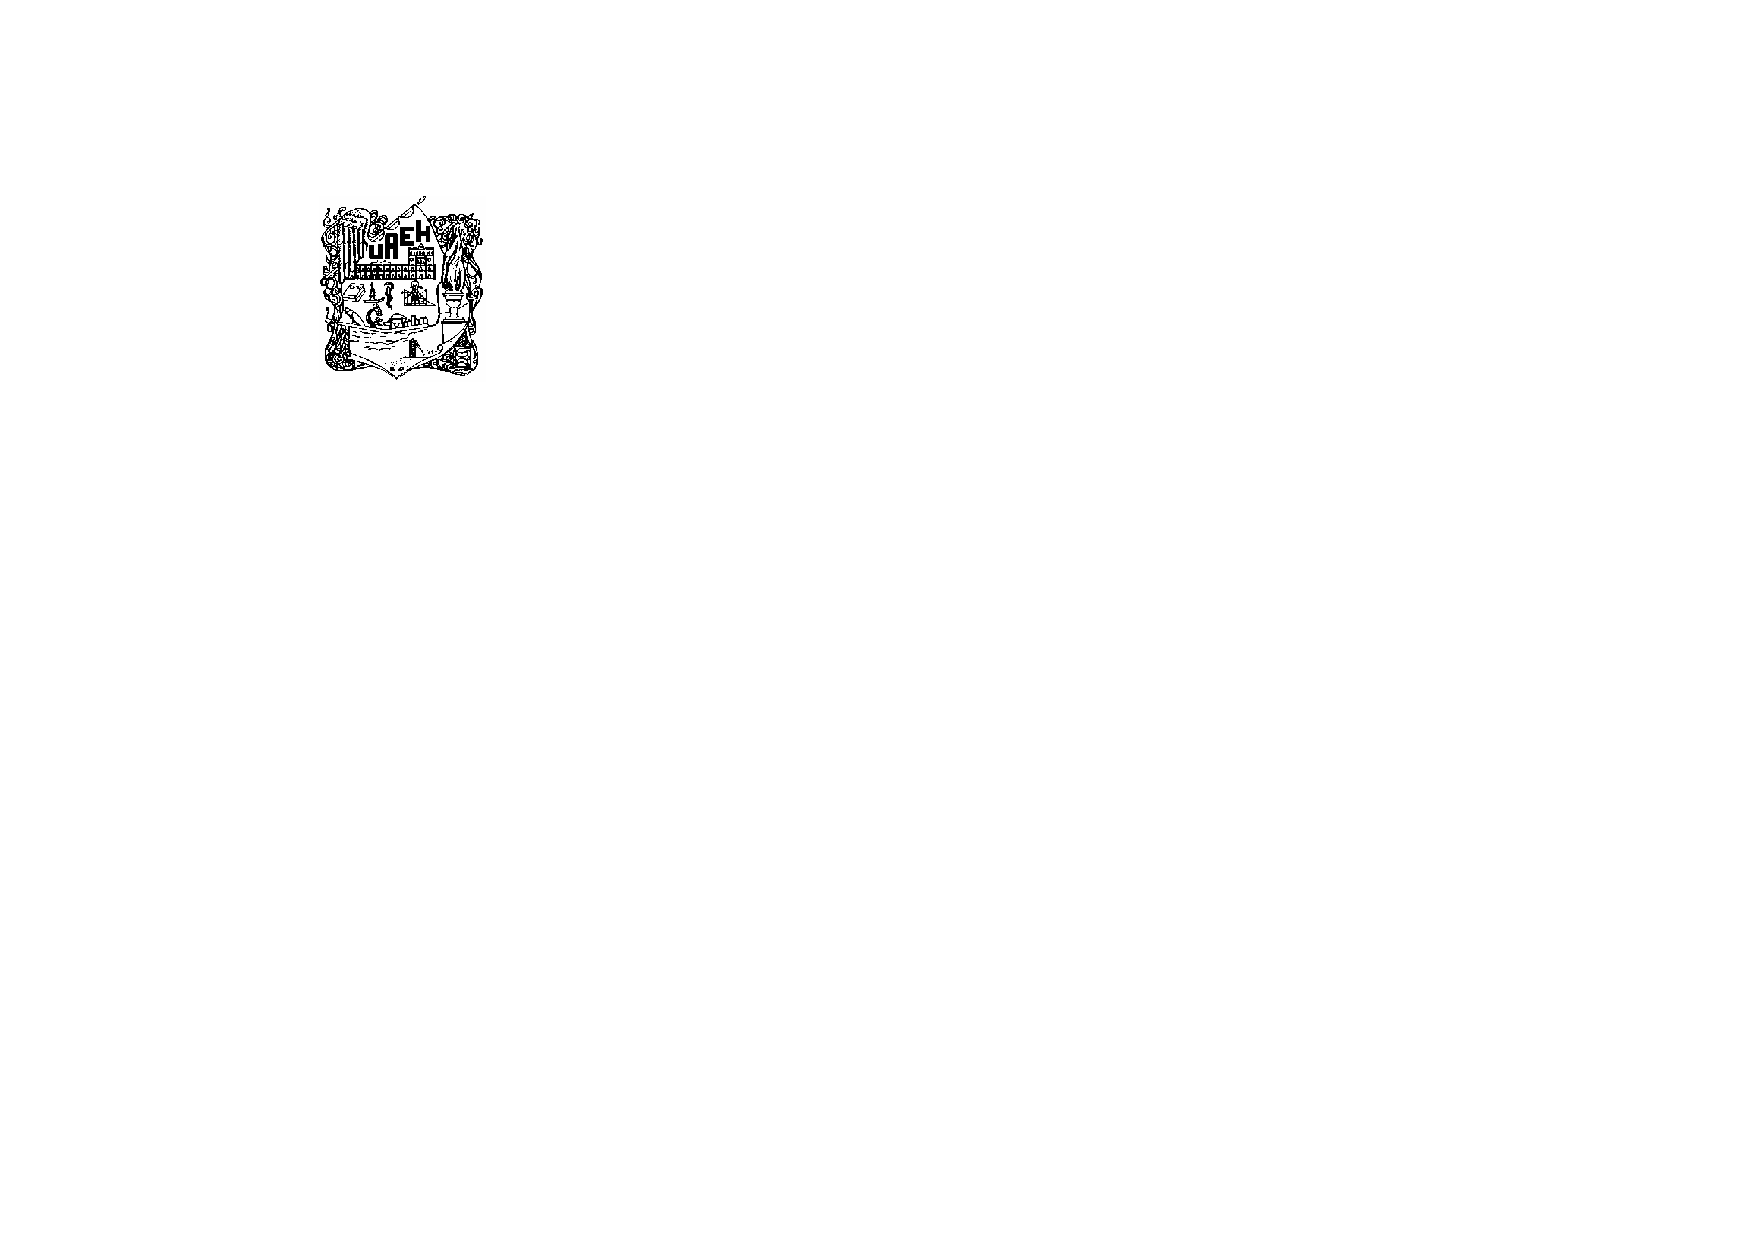
\includegraphics[scale=1.2,bb=55 20 0 0]{escudouaeh.pdf}

    \vspace*{2cm}

    \textsc{Universidad Autónoma del Estado de Hidalgo}

    \textsc{Instituto de Ciencias Básicas e Ingeniería}

    \textsc{Área Académica de Matemáticas y Física}

    \vspace*{2cm}

    \textbf{\Huge Buscando Jaulas}

    \vspace*{2cm}

    {\large Tesis que para obtener el título de}

    \vspace*{2cm}

    \textsc{Licenciada en Matemáticas Aplicadas}

    {\large presenta}

    \vspace*{2cm}

    {\Huge Citlalli Zamora Mejía}

    \bigskip

    {\large bajo la dirección de}

    \bigskip

    {\Large Dr.~Rafael Villarroel Flores}

    \bigskip

    {Pachuca, Hidalgo. Junio de 2013.} \\

  \end{center}
\end{titlepage}




\chapter*{Agradecimientos}
Aquí van los agradecimientos



\newpage \thispagestyle{empty}




\chapter{Introducción}

En matemáticas, los problemas de minimización son muy comunes.
En teoría de gráficas, la búsqueda de jaulas es un ejemplo de
ello: consiste en encontrar gráficas regulares, con cuello dado,
pero con la menor cantidad de vértices posibles.


La presente tesis aborda el problema de jaulas 3-regulares de
cuello dado. Primero presenta una construcción de dichas jaulas de
cuello menor o igual a doce, de las cuales se sabe la
cantidad de vértices que tienen y si son únicas o no. Si el cuello
es mayor, se conocen cotas inferiores y superiores; pero todavía
no se sabe si las gráficas son jaulas, y mucho menos si son
únicas.  La segunda parte, presenta un método computacional; el
cual dibuja gráficas $3$-regulares de cuello par, a partir de un
listado de grupos; e identifica si alguna iguala o reduce la cota
superior.


El método que se sigue, en la segunda parte, tiene dos niveles. El
primero, construye gráficas de Cayley localmente $3K_2$, las
cuales son vértice-transitivas, y basta con hacer un análisis al
rededor de la identidad para saber como se comporta en el resto de
los vértices. El segundo nivel, dibuja la bipartita clánica,
asociada a cada una de las gráficas de Cayley localmente $3K_2$,
construidas en el paso anterior. En dicha gráfica, por cada
vértice y por cada clan, de la gráfica original; existe un vértice
asociado a \'el: en donde los vértices $x,y$ son adyacentes si y
solo si $x$ es un vértice de la gráfica de Cayley y $y$ un clan
que contenga a $x$ o viceversa.

Para construir gráficas de Cayley es necesario trabajar con
grupos, y dado que $GAP$ es un software libre especializado; que
contiene una amplia lista de ellos, se utiliza para hacer el
programa antes mencionado.



\tableofcontents




\chapter{Conceptos básicos}

Antes de comenzar con el tema principal del presente trabajo, es
necesario introducir algunos conceptos, unos mas básicos y comunes
que otros, pero necesarios para facilitar la comprensión del
lenguaje que se maneja. Así como resultados ya existentes que
servirán de ayuda en la justificación del análisis que se hace a las
gráficas de Cayley 3-regulares.


\section{Grupos}

En esta sección se encuentran definiciones básicas de grupos y
algunos resultados elementales que no serán demostrados. Si
el lector se interesa puede consultar más acerca del tema en
$\cite{Barrera}$, $\cite{Ehrlich}$, $\cite{Hall}$ y $\cite{Zaldivar}$.

\begin{definition}{\textbf{Grupo}}\\\index{Grupo} Un grupo es una
pareja ($G$,$\circ$), con $G$ un conjunto no vacío, $\circ$ una
función de $G\times G \rightarrow G$ llamada operación binaria y
denotada por $\circ (x,y):=x\circ y$, la cual satisface:

\begin{enumerate}
\item La operación $\circ$ es asociativa, es decir, $g_1\circ
  (g_2\circ g_3)=(g_1 \circ g_2)\circ g_3$ para todos
  $g_1,g_2,g_3\in G$.
\item Existe $e\in G$ tal que $e\circ g_1=g_1$, para todo
  $g_1\in G$, llamado neutro por la izquierda.
\item Dado $g_1\in G$, existe $g_1'\in G$ tal que $g_1'\circ g_1
  = e$, a dicho elemento se le conoce como inverso por la
  izquierda y se denota por $g_1^{-1}$.
\end{enumerate}
\end{definition}


Apartir de este momento, la notación $g_1\circ g_2$ ser\'a
sustituida por $g_1g_2$ pues es m\'as cómodo dejar de escribir
$\circ$. 



\begin{theorem}\label{gg=g}
  Sean $G$ un grupo y $g$ un elemento de él, si $gg=g$ entonces $g$ es
  igual a la identidad.
\end{theorem}

\begin{proof}
 Como $g\in G$ entonces existe un elemento $g'\in G$ tal
que $g'g=e$ y como $gg=g$ se tiene
\begin{equation*}
  \begin{split}
    e=g'g&=g'(gg)\\
    &=(g'g)g=eg=g
  \end{split}
\end{equation*}

concluyendo la demostración.
\end{proof}

Se puede demostrar que tanto el elemento neutro, como el inverso son
únicos, además se tiene que:
\begin{equation*}
\begin{split}
eg&=ge=e\\ 
& \textit{    y   }\\
 g^{-1}g&=gg^{-1}=e
\end{split}
\end{equation*}
para todo  $g$ del grupo $G$. Si se desea, se puede consultar la demostración
en $\cite{Barrera}$.

\begin{example}\textbf{Grupo simétrico o de
    permutaciones}\\\index{Grupo simétrico}\index{Grupo de permutaciones}
  Sea $S_n$\index{$S_n$} el conjunto formado por todas las funciones
  biyectivas del conjunto $\{1,2,...,n \}$ en sí mismo. Entonces $S_n$ es un
  grupo con respecto a la composición de funciones.


\begin{proof}

Dado que la operación es la composición de funciones, se sabe que las
tres condiciones necesarias par ser grupo, se cumplen. 
\end{proof}

  $S_n$ se denomina grupo simétrico de grado $n$ y sus elementos son
  conocidos como permutaciones del conjunto $\{1,2,...,n\}$.
\end{example}

Sea $\sigma \in S_n$ la permutación que manda el elemento $j$ a $j+1$
y $n$ a $1$, con $j=1,2,...,n-1$, ésta permutación se denota como
$(12...n)$. Una misma permutación tiene varias representaciones pues
$(23...n1)$ es la permutación $\sigma$.

Las permutaciones pueden dejar fijos algunos elementos, $(1n)$ manda
$1$ a $n$ y $n$ a $1$, dejando fijos a todos los demás. En general
$(i_1i_2...i_k)$, con $i_j\in \{ 1,2,...,n\}$ y $k\le n$, es tal que
manda $i_j$ a $i_{j+1}$ e $i_k$ a $i_1$.

\begin{definition}\textbf{Grupo abeliano}\\\index{Grupo abeliano}
  Sea $G$ un grupo, si para todo $g_1,g_2\in G$ se cumple que
  $g_1g_2=g_2g_1$ entonces $G$ recibe el nombre de grupo abeliano.
\end{definition}


\begin{definition}\textbf{Subgrupo}\\\index{Subgrupo}
  Sea $G$ un grupo y $H$ un conjunto no vacío de $G$. Se dice que $H$
  es un subgrupo si la operación de $G$ restringida a $H$ hace de
  \'este un grupo y se denota como $H\le G$.
\end{definition}


\begin{theorem}\label{subgrupo}
  Sean $G$ un grupo y $H$ un subconjunto no vacío de $G$. Entonces las
  siguientes condiciones son equivalentes:
  \begin{enumerate}
  \item $H$ es un subgrupo de $G$
  \item \begin{enumerate}
    \item Para todo $x,y \in H$, $xy\in H$
    \item Para todo $x\in H$, $x^{-1}\in H$
    \end{enumerate}
  \item Para todo $x,y \in H$ se tiene $xy^{-1}\in H$
  \end{enumerate}\label{teonodemos}
\end{theorem}

\begin{proof}
  La demostración del teorema~\ref{teonodemos} se encuentra en
  \cite{Barrera}, página 24; o en \cite{Ehrlich}, página 44.
\end{proof}

\begin{theorem}
Sea $G$ un grupo. La intersección de subgrupos de $G$ es también un subgrupo. 
\end{theorem}

\begin{proof}
Sea $I$ un conjunto de subgrupos de $G$. 

Primero; cada subgrupo $H$ en el conjunto $I$, contiene a la identidad,
$e$, de $G$, por ser un subgrupo. Entonces se tiene que
$e\in \bigcap_{H\in I}H$, con lo que se puede concluir que la
intersección de los elementos de $I$, es no vacía.

Ahora, sean $a,b\in \bigcap_{H\in I}H$. Entonces $a,b\in H$,
para cada $H$ en $I$. Por el teorema~\ref{teonodemos}, se tiene
$ab^{-1}\in H$, para cada $H\in I$, de lo que se sigue $ab^{-1}\in
\bigcap_{H\in I}H$.

Nuevamente, usando el teorema~\ref{teonodemos}, se concluye que la
intersección de subgrupos de $G$ es también un subgrupo de $G$.
\end{proof}

\begin{definition}\textbf{Subgrupo generado por un conjunto}\\\index{Subgrupo generado}
  Sean $G$ un grupo y $S$ un conjunto no vacío de $G$. Entonces el
  subgrupo de $G$ generado por $S$ es:
\begin{equation*}
\langle S \rangle := \bigcap_{\text{$H\le G$ tal que $S \subset H$}}H
\end{equation*}\index{$\langle S \rangle$}
\end{definition}

\begin{definition}\textbf{Orden del grupo}\\\index{Orden del grupo}
  El orden de un grupo $G$, es el número de elementos que tiene; y es
  denotado por $|G|$.
\end{definition}

La definición no pide que el orden de un grupo sea finito, pero
para fines de esta tesis sólo se consideran éste tipo de grupos, a los
cuales se les conoce como grupos finitos.\index{Grupos finitos}

\begin{definition}\textbf{Orden de un elemento}\\\index{Orden de un elemento del grupo}
  Sean $G$ un grupo y $g\in G$, el orden de $g$ es el menor entero
  positivo $n$ tal que $g^n=e$ y se denotará por $|g|=n$.\index{$|g|$}
\end{definition}

\begin{definition}{\textbf{Homomorfismo}}\\\index{Homomorfismo de
    grupos} Sean $(G,\circ)$ y ($G_1, \ast$) dos grupos. 
Un homomorfismo entre $G$ y $G_1$ es una función $f : G \rightarrow G_1$, tal que $f(x\circ
  y)=f(x)\ast f(y)$ para todo $x,y\in G$.
\end{definition}

\begin{definition}\textbf{Isomorfismo de grupos}\\\index{Isomorfismo de grupos}
  Sean $(G,\circ)$ y ($G_1, \ast$) dos grupos. Si existe $f : G
  \rightarrow G_1$, una función biyectiva tal que $f(x\circ
  y)=f(x)\ast f(y)$ para todo $x,y\in G$. Entonces se dice que $G$ es
  isomorfo a $G_1$ y se denota como $G\cong G_1$. Además a $f$ se le
  conoce como un isomorfismo entre $G$ y $G_1$.
\end{definition}


\begin{definition}\textbf{Automorfismo de un grupo}\\\index{Automorfismo de un grupo}
  Un isomorfismo, de un grupo en sí mismo es llamado automorfismo.
\end{definition}

\begin{definition}\textbf{Órbita}\\\index{Órbita}
  Sea $G$ un grupo y $x\in G$, la órbita de $x$ se define como el
  conjunto $\orb (G,x)$.
  \begin{equation*}
    \orb(G,x):=\{ gx \mid g\in G \}
  \end{equation*}
\end{definition}

\begin{definition}\textbf{Estabilizador}\\\index{Estabilizador}
  Sea $G$ un grupo y $x\in G$, el estabilizador de $x$ en $G$, se define
  como:

\begin{equation*}
  \Stab (G,x)=\{ g\in G \mid gx=x \}
\end{equation*}
\end{definition}

Sea $Hg=\{hg \mid h\in H\}$, definimos el índice\index{Índice de un
  subgrupo} de un subgrupo $H$ como la cardinalidad del conjunto $\{Hg
\mid g\in G \}$ y se denota por $[G:H]$. A $Hg$ se le conoce como la
clase lateral derecha de $H$ en $G$, representada por $g$\index{Clase
  lateral}.

%Las definiciones de índice y clase lateral, se mencionen de manera muy
%rápida y poco formal pues lo que realmente se busca es poder llegar al
%siguiente teorema.

\begin{theorem}\textbf{Teorema de Lagrange}\\\index{Teorema de Lagrange}
  Si $H$ es un subgrupo de un grupo finito $G$, entonces
$$|G|=|H|[G:H]$$
\label{TeoLagrange}
\end{theorem}

El teorema~\ref{TeoLagrange} es un resultado muy importante en teoría
de grupos, pues establece una relación entre el orden del grupo y el
orden de sus subgrupos. No ser\'a demostrado pero si el lector esta
interesado puede consultar la demostración en \cite{Barrera} y \cite{Ehrlich}.


\begin{definition}\textbf{Acción de un grupo}\\\index{Acción de un grupo}
  Sean $G$ un grupo y $X$ un conjunto, $G$ actúa en $X$ si existe una
  función $\varphi: G \times X \rightarrow X$, $\varphi (g,x)
  \rightarrow gx$ tal que:

  \begin{enumerate}
  \item $ex=x$, con $e$ la identidad en $G$ y $x\in X$.

  \item $g_1(g_2x)=(g_1g_2)x$, con $g_1,g_2 \in G$ y $x\in X$.
  \end{enumerate}
\end{definition}


\begin{definition}\textbf{Acción transitiva}\\\index{Acción transitiva}
  Un grupo $G$, actúa transitivamente en un conjunto $X$, si para todo
  par de elementos $x_1, x_2 \in X$, existe $\sigma \in G$ tal que $\sigma (x_1) = x_2$.
\end{definition}



\begin{definition}\textbf{Acción regular}\\\index{Acción regular}
  Sea $G$ un grupo y $X$ un conjunto, tal que $G$ actúa en él. Se dice que la acción es regular, o
  que $G$ actúa regularmente en $X$ si:
  \begin{enumerate}
  \item La acción es transitiva
  \item $|\Stab (G,x)|=1$, para toda $x\in X$
  \item $|G|=|X|$
  \end{enumerate}
\end{definition}


\begin{example}
  Sea $G=\{ (123),(132),(1)\}$ subgrupo del grupo de permutaciones $S_3$, entonces $G$
  actúa regularmente en el conjunto $X=\{ 1,2,3\}$.
\begin{proof} Para que la acción sea regular se deben probar tres cosas:

  \begin{enumerate}
  \item La acción es transitiva
    \begin{enumerate}
    \item Para $1,2\in X$, la permutación $(123)$ manda $1$ a $2$ y la
      permutación $(132)$ manda $2$ a $1$.
    \item Para $1,3\in X$, $(132)$ manda $1$ en $3$ y $(123)$ manda
      $3$ a $1$.
    \item Para $2,3\in X$, $(123)$ manda $2$ en $3$ y $(132)$ manda
      $3$ a $2$.
    \end{enumerate}
  \item $|\Stab (G,x)|=1$ para todo $x$
    \begin{enumerate}
    \item Para $1\in X$, $|Stab (G,1)|=1$
    \item Para $2\in X$, $|Stab (G,2)|=1$
    \item Para $3\in X$, $|Stab (G,3)|=1$
    \end{enumerate}
  \item $|G|=3=|X|$
  \end{enumerate}
  Por lo tanto $G$ actúa regularmente en $X$.
\end{proof}
\end{example}


Si un grupo $G$ actúa regularmente en un conjunto $X$ entonces, si $x \in X$
\begin{equation*}
  |G|=\frac{|G|}{|\Stab(G,x)|}
  = | \orb (G,x)|=|X|
\end{equation*}

De hecho, para verificar que $G$ actúa regularmente en $X$, basta
probar una de las tres condiciones para que las otras se cumplan, pero
este resultado no será demostrado aquí.

\section{Gráficas}

En la sección anterior se habló acerca de grupos, una rama de las
matemáticas bastante más común que la presente sección. Seguramente
algunas de las definiciones aquí presentadas serán conocidas, pero tal
vez otras no.

Aquí se encuentran las definiciones necesarias de teoría de gráficas,
así como algunos resultados y sus demostraciones. Si el lector se
interesa en conocer más acerca de teoría de gráficas puede consultar
\cite{Harary}.

\begin{definition}\textbf{Gráfica}\\\index{Gráfica}
  Una gráfica $\Gamma$ es un par ordenado de conjuntos,
  $\Gamma=\{V(\Gamma),E(\Gamma)\}$, donde $V(\Gamma)$ es finito,
  llamado vértices\index{Vértice} de $\Gamma$, y
  \begin{equation*}
    E(\Gamma) \subseteq
    V(\Gamma)^{(2)}:=\{e\subseteq V(\Gamma) \mid |e|=2\}
  \end{equation*}
\end{definition}

A los elementos de $E(\Gamma)$ se les conoce como
aristas\index{Arista}.

La definición general de una gráfica permite que $V(\Gamma)$ sea
infinito, y $E(\Gamma)$ es definido de tal forma que sus elementos
pueden ser dirigidos\index{Arista dirigida}; incluso pueden existir
lazos\index{Lazos}: aristas que van de un vértice en sí mismo. Pero
para fines de esta tesis es suficiente definirla con vértices finitos,
aristas no dirigidas y sin lazos.

\begin{definition}\textbf{Complemento de una gráfica}\\\index{Complemento de una gráfica}
  Sea $\Gamma$ una gráfica. Se define el complemento de
  $\Gamma$, $\overline{\Gamma}$, como:

  \begin{equation*}
    \begin{split}
      V(\overline{\Gamma})&=V(\Gamma)\\
      E(\overline{\Gamma})&=V(\Gamma)^{(2)}\setminus E(\Gamma)
    \end{split}
  \end{equation*}

\end{definition}



\begin{definition}\textbf{Orden de una gráfica}\\\index{Orden de una gráfica}
  El orden de una gráfica $\Gamma$ se define como $|\Gamma|:= |V(\Gamma)|$.
\end{definition}

\begin{definition}\textbf{Vértices adyacentes}\\\index{Vértices adyacentes}
  Sea $\Gamma$ una gráfica, si $x , y \in V(\Gamma)$ tal que
  $\{x,y\}\in E(\Gamma)$ se dice que $x$ y $y$ son adyacentes.
\end{definition}


La forma de denotar que dos vértices $x$ y $y$, son adyacentes es
$x\thicksim y$. En algunas ocasiones, aunque de manera no tan formal,
también se dice que $x$ es vecino o amigo de $y$.\index{Amigos de un
  vértice}\index{Vecinos de un vértice}


Las gráficas se representan frecuentemente como un dibujo, pero
dos dibujos a pesar de ser aparentemente distintos pueden estar
representando la misma gráfica. Incluso si dos gráficas están siendo
representadas por conjuntos, y estos son diferentes, se puede estar
hablando de la misma gráfica.

\begin{definition}\textbf{Isomorfismo}\\\index{Isomorfismo}
  Sean $\Gamma_1,\Gamma_2$ dos gráficas. Un isomorfismo de
  $\Gamma_1,\Gamma_2$ es una función biyectiva $f:
  V(\Gamma_1)\rightarrow V(\Gamma_2)$ tal que $x\thicksim y$ en
  $\Gamma_1$ si y solo si $f(x)\thicksim f(y)$ en $\Gamma_2$.
\end{definition}


\begin{definition}\textbf{Gráficas isomorfas}\\\index{Gráfica isomorfa}
  Sean $\Gamma_1,\Gamma_2$ dos gráficas, si existe un isomorfismo
  entre $\Gamma_1$ y $\Gamma_2$, se dice que $\Gamma_1$ y $\Gamma_2$
  son isomorfas.
\end{definition}


\begin{definition}\textbf{Automorfismo}\\\index{Automorfismo}
  Un isomorfismo de una gráfica $\Gamma$ en si misma, se llama automorfismo de
  $\Gamma$.
\end{definition}



\begin{proposition}\textbf{Grupo de Automorfismo de una gráfica}\\\index{Grupo de automorfismos}
  Sea $n$ el orden de una gráfica $\Gamma$. Entonces, el conjunto
  de todos los automorfismos de $\Gamma$, es un subgrupo de $S_n$,
  denotado $\Aut(\Gamma)$, llamado grupo de automorfismos de $\Gamma$.
\end{proposition}

\begin{proof} Los automorfismos de $\Gamma$ pertenecen a $S_n$
  y la identidad es un automorfismo, por lo que el conjunto de
  automorfismos de $\Gamma$ no es vacío. Sean $\phi$ y $\psi$
  automorfismos de $\Gamma$ y sean $x,y\in V(\Gamma)$ tales que $x\sim
  y$ entonces $\phi(x)\sim \phi(y)$ y ambos están en $V(\Gamma)$,
  aplicando $\psi$:
\begin{equation*}
  \psi(\phi(x))\sim \psi(\phi(y))
  \mbox{ es decir } 
  (\psi \circ \phi) (x)\sim (\psi \circ \phi)(y)
\end{equation*}

Por lo que $(\psi \circ \phi)$ es también un automorfismo de
$\Gamma$. Por lo tanto el grupo de automorfismos de $\Gamma$ es un
subgrupo de $S_n$.
\end{proof}

\subsection{Familias de gráficas}

Las gráficas pueden clasificarse en familias de acuerdo a sus
características. Esta sección presenta algunas de estas
clasificaciones.

\begin{definition}\textbf{Gráfica completa}\\\index{Gráfica completa}
  La gráfica con $n$ vértices y todas las aristas posibles se llama
  gráfica completa y se denota $K_n$\index{$K_n$} con $n\geq 1$.
\end{definition}

\begin{definition}\textbf{Gráfica $P_n$}\\\index{$P_n$}
  Los vértices de la gráfica $P_n$ son $V(P_n):=\{v_1,v_2,...,v_n\}$ y
  las aristas $E(P_n):=\{v_i \sim v_{i+1} \mid i<n\}$. La
  figura~\ref{P5} es la gráfica $P_5$.
\end{definition}


\begin{figure}
  \centering
  \begin{tikzpicture}
    \SetVertexNoLabel

    \SetUpVertex[MinSize=1.5pt] \grPath[RA=2.5,prefix=v]{5} { \foreach
      \y in {0,1,...,4} { \setcounter{in}{\y+1} \stepcounter{in} \draw
        (v\y) node[below right]{$v_{\y}$}; }}

  \end{tikzpicture}
  \caption{$P_5$} \label{P5}
\end{figure}



\begin{definition}\textbf{Unión disjunta}\\\index{Unión disjunta}
  Dadas dos gráficas $G$ y $H$, se define la unión disjunta $G\cup H$
  como;
$$V(G\cup H):=V(G)\dot{\cup}V(H)$$ $$E(G\cup H):=E(G)\dot{\cup}E(H)$$
\end{definition}

La unión de una gráfica $G$ con si misma se denota por $2G$. En general la unión
disjunta de $G$, $n$ veces, es denotada por $nG$. \index{$nG$}

El símbolo $\dot{\cup}$ representa la unión de conjuntos, pero de
forma disjunta; esto es, si $|V(G)|=n$ y $|V(H)|=m$ entonces
$|V(G)\dot{\cup}V(H)|= n + m$. Si $v \in V(G)\dot{\cup}V(H)$ entonces
$v$ esta estrictamente en $V(G)$ o en $V(H)$.


\begin{definition}\textbf{Gráfica $nK_m$}\\\index{Gráfica $nK_m$}
  A la unión disjunta de $n$ gráficas completas con $m$ vértices, $K_m$, se le denota por $nK_m$
\end{definition}


\begin{definition}\textbf{Subgráfica}\\\index{Subgráfica}
  Una gráfica $H$ es subgráfica de $G$ si $V(H)\subseteq V(G)$ y
  $E(H)\subseteq E(G)$.
\end{definition}


\begin{definition}\textbf{Clan}\\\index{Clan}
  Un clan es una subgráfica completa maximal.
\end{definition}

Es decir, es una subgráfica completa $H$, a la cual no se le puede
agregar ningún otro vértice, que no esté en ella, con las
correspondientes aristas entre \'el y los vértices de \'esta, que
hagan que la nueva gráfica sea completa.

\begin{example}
  Los clanes de la gráfica~\ref{grafclan}, son las subgráfica de la
  figura~\ref{clanes}. Tiene un clan isomorfo a $K_4$ y cuatro
  isomorfos a $K_3$.


\begin{figure}[htb]
  \centering
  \begin{tikzpicture}
    \SetVertexNoLabel

    \SetUpVertex[MinSize=1.5pt] \grCycle[RA=2.5,prefix=v]{8} {
      \foreach \y in {0,1,...,7} { \setcounter{in}{\y}
        \stepcounter{in} \draw (v\y) node[below right]{$\alph{in}$};
      }} \Edges(v1,v3,v7,v1,v5,v3) \Edges(v5,v7)

  \end{tikzpicture}
  \caption{} \label{grafclan}
\end{figure}




\begin{figure}
  \centering
  \begin{tikzpicture}
    \SetVertexNoLabel \SetUpVertex[MinSize=1.5pt]

    \grEmptyPath*[x=0,y=0,RA=2,prefix=v]{,,,,,}
    \grEmptyPath*[x=1,y=2,RA=4,prefix=w]{,,}
    \grEmptyPath*[x=0,y=3,RA=2,prefix=x]{,,,}
    \grEmptyPath*[x=0,y=5,RA=2,prefix=y]{,} \Vertex[x=5,y=5]{z0}
    \Edges(v0,v1,w0,v0) \Edges(v2,v3,w1,v2) \Edges(x0,x1,y1,x0,y0,x1)
    \Edges(y0,y1) \Edges(x2,x3,z0,x2) \Edges(v4,v5,w2,v4)

    \draw (v0) node [below]{$f$}; \draw (v1) node[below right]{$d$};
    \draw (w0) node[below right]{$e$}; \draw (v2) node[below
    right]{$b$}; \draw (v3) node[below right]{$h$}; \draw (w1)
    node[below right]{$a$}; \draw (v4) node[below right]{$f$}; \draw
    (v5) node[below right]{$h$}; \draw (w2) node[below right]{$g$};
    \draw (x0) node[below right]{$f$}; \draw (x1) node[below
    right]{$h$}; \draw (y0) node[below right]{$d$}; \draw (y1)
    node[below right]{$b$}; \draw (z0) node[below right]{$c$}; \draw
    (x2) node[below right]{$d$}; \draw (x3) node[below right]{$b$};
  \end{tikzpicture}
  \caption{Clanes de la figura~\ref{grafclan}.}\label{clanes}
\end{figure}
\end{example}


\begin{definition}\textbf{Bipartita}\\\index{Bipartita}
  Sea $B$ una gráfica, si existen conjuntos no vacíos $X$ y $Y$ de
  $V(B)$ tales que
  \begin{enumerate}
  \item $V(B)=X\cup Y$ y $X\cap Y=\phi$.
  \item Si $x\sim y$ entonces $x\in X$ y $y\in Y$ o viceversa.
  \end{enumerate}
  entonces a $B$ se le conoce como gráfica bipartita.
\end{definition}

En este caso, se dice que los conjuntos $X$ y $Y$ son una
bipartición\index{Bipartición} de $B$ y se denota por $B(X,Y)$. Además
los vértices de $B$ se pueden colorear con dos colores, sin que una
arista tenga el mismo color en ambos extremos. Si los vértices en $X$
se colorean con el color uno, y los de $Y$ con el dos, se tiene lo
deseado, pues no existe arista entre dos elementos del mismo conjunto.



\begin{definition}\textbf{Bipartita completa}\\\index{Bipartita completa}
  Dados $m,n\geq 1$, la gráfica bipartita completa $K_{m,n}$ se define
  como $$K_{m,n}:=\overline{K_m \cup K_n}$$
\end{definition}


\begin{definition}\textbf{Bipartita clánica}\\\index{Bipartita clánica}
  Sea $Cl_G:=\{H \mid H$ es un clan de una gráfica $G \}$. Se define
  la gráfica bipartita clánica $BC_G$, de una gráfica $G$,
  como $$V(BC_G) := V(G) \dot{\cup} Cl_G$$ Donde $x,y\in V(BC_G)$ son
  adyacentes si y solo si $x\in V(G)$ y $y$ es un clan de $G$, tales
  que $x\in y$ o viceversa.
\end{definition}

Es decir, la gráfica bipartita clánica es aquella cuyos
vértices están asociados a los elementos de $V(G)$ y a los clanes de
$G$, de manera disjunta. Donde las aristas que existen se dan solo
entre un elemento asociado a un vértices y otro asociado a un clan. La
figura~\ref{BCG} es la gráfica bipartita clánica de la
gráfica~\ref{grafclan}.

\begin{figure}
  \centering
  \begin{tikzpicture}[scale=0.85]
    \SetVertexNoLabel \SetUpVertex[MinSize=1.5pt]

    \grEmptyPath*[x=0,y=3,RA=2,prefix=v]{,,,,,,,}
    \grEmptyPath*[x=1,y=0,RA=3,prefix=w]{,,,,}

    { \foreach \y in {0,1,...,7} { \setcounter{in}{\y}
        \stepcounter{in} \draw (v\y) node[above right]{$\alph{in}$};
      }}

    \Edges(v0,w0,v1,w0,v7) \Edges(v1,w1,v2,w1,v3)
    \Edges(v3,w3,v4,w3,v5) \Edges(v5,w4,v6,w4,v7)
    \Edges(v1,w2,v3,w2,v5,w2,v7) \draw(1,-.5) node {$K_3$};
    \draw(4,-.5) node {$K_3$}; \draw(7,-.5) node {$K_4$};
    \draw(10,-.5) node {$K_3$}; \draw(13,-.5) node {$K_3$};
  \end{tikzpicture}
  \caption{Gráfica bipartita clánica de~\ref{grafclan}}\label{BCG}
\end{figure}

\begin{definition}\textbf{Subgráfica inducida}\\\index{Subgráfica inducida}
  Una subgráfica $H$ de una gráfica $G$ se dice inducida si:
\begin{equation*}
\{x,y\}\in
  V(H)^{(2)}\cap E(G) \text{ entonces } \{x,y\}\in E(H)
\end{equation*}
\end{definition}

Una subgráfica inducida esta determinada por su conjunto de
vértices. Si $X\subset V(G)$, la subgráfica de $G$ inducida por $X$ se
denota por $G[X]$.

\begin{proposition}\textbf{}\\
  Si $G$ y $H$ son gráficas isomorfas, y la gráfica $L$ es subgráfica
  de $G$; entonces $H$ tiene una subgráfica isomorfa a $L$.
\end{proposition}

\begin{proof}
 Sea $\varphi : G \rightarrow H$ un isomorfismo entre G y
H, una subgráfica de $H$ isomorfa a $L$ es la gráfica inducida por
$\varphi (V(L))$, si $x\sim y$ en $L\subset G$ entonces $\varphi
(x)\sim \varphi (y)$ en H.
\end{proof}

\subsection{Caminos y Ciclos}



\begin{definition}\textbf{Camino de longitud $n$}\\\index{Camino de longitud $n$}
  Un camino de longitud $n$, en una gráfica $G$, es una sucesión de vértices de
  $G$, todos distintos entre sí, tal que $v_i\sim v_{i+1}$ para
  $i=0,1,...,n-1$. Se dice que es un
  ``$v_0v_n$-camino''.\index{$v_0v_n$-camino}

\end{definition}


\begin{definition}\textbf{Gráfica conexa}\\\index{Gráfica conexa}
  Una gráfica $G$ es conexa si para todos $ u,v\in V(G)$ con $u\neq
  v$, existe un $uv$-camino de longitud $n$.
\end{definition}

\begin{proposition}\textbf{}\\
  Sea $G$ una gráfica. Si existe un $uv$-camino en $G$, entonces también existe un $vu$-camino. Más aún la
  relación $\simeq$ en $V(G)$ dada por $u\simeq v$ si y solo si existe
  un $uv$-camino en $G$, es una relación de equivalencia.
\end{proposition}
\begin{proof} Sea $\{u=t_0,t_1,t_2,...,t_n=v \}$ un $uv$-camino
en $G$, entonces $\{v=t_n,...,t_1,t_0=u \}$ es un $vu$-camino. Por lo tanto, si existe un $uv$-camino siempre existe un $vu$-camino.

 Ahora se demostrará que es una relación de equivalencia.

\begin{enumerate}

\item Reflexividad: $x\simeq x$, $\{ x\}$ es el $xx$-camino.

\item Simetría: si $x \simeq y$ entonces $y \simeq x$. Como existe un $xy$-camino entonces existe un
  $yx$-camino.

\item Transitividad: Si $x \simeq y$ y $y \simeq z$ entonces $x \simeq
  z$.  Sabemos que existen $\{x=t_0,...,t_n=y\}$ y
  $\{t_n=y,t_{n+1},...,t_m=z \}$ los caminos entre $x$,$y$, y $y$,$z$
  respectivamente, entonces $ t_0, t_1,...,t_n,...t_m$ es un recorrido
  entre $x$ y $z$. Sea $i$ el subíndice mas pequeño tal que $t_i =
  t_j$ con $i=0,...,m-1$ y $j =1,...,m$ entonces
  $x=t_0,...,t_i,t_{j+1},...,t_m=z$ es un $xz$-camino.
\end{enumerate}

Por lo tanto $\simeq$ es una relación de equivalencia.
\end{proof}

\begin{definition}\textbf{Distancia}\\\index{Distancia}
Sea $G$ una gráfica y sean $u,v\in V(G)$. La distancia entre $u$ y $v$, $d(u,v)$, si existe
  un $uv$-camino se define como:
  \begin{equation*}
    d(u,v)=\min\{ \text{longitud $p$}  \mid \text{$p$ es un $uv$-camino} \}
  \end{equation*}

  o $d(u,v)=\infty$ si no existe dicho camino.
\end{definition}

\begin{definition}\textbf{Ciclo}\\\index{Ciclo}
  Sea $G$ una gráfica, un ciclo en $G$ de longitud $n$ es una sucesión
  de vértices $v_1,...,v_n$ todos distintos entre sí, tales que
  $v_1,...,v_n$ es un camino y $v_1 \sim v_n$ ($n\geq 3$).
\end{definition}

Los ciclos de longitud $n$ se conocen como $n$-ciclos y si el ciclo es
de longitud par o impar se llaman ciclos pares o impares
respectivamente.

\begin{definition}\textbf{Árbol}\\\index{Árbol}
  Un árbol es una gráfica conexa, sin ciclos.
\end{definition}

\begin{definition}\textbf{Cuello}\\\index{Cuello}
  Sea $G$ una gráfica con ciclos. Se define el cuello de $G$ como:
  \begin{equation*}
    g(G):= \min\{ \text{longitud $c$} \mid  \text{$c$ es un ciclo en $G$} \}
  \end{equation*}
\end{definition}

Los árboles y la unión disjunta de ellos, son las únicas gráficas
que no tienen cuello.

\begin{definition}\textbf{Diámetro}\\\index{Diámetro}
  Sea $G$ una gráfica, el diámetro de $G$ es:
  \begin{equation*}
    \diam(G):=\max\{ d(u,v) | u,v \in V(G)\}
  \end{equation*}
\end{definition}

\begin{definition}\textbf{Vecindad de $x$}\\\index{Vecindad de $x$}
  Sean $G$ una gráfica y $x\in V(G)$, la vecindad de $x$,
  $N_G(x)$\index{$N_G(x)$}, es la subgráfica de $G$ inducida por
  $\{y\in V(G) \mid y\sim x\}$.
\end{definition}

\begin{proposition}\textbf{}\\
  No existe una gráfica $G$ tal que la vecindad de $x$ sea isomorfa al camino de longitud dos, para todo $ x\in  V(G)$.
\end{proposition}

\begin{proof} Se demostrará por contradicción. Suponga que existe una gráfica $G$, tal que la vecindad de cualquiera de sus vértices es isomorfa a $P_2$. 

Sea $x\in V(G)$ y sean $a$, $b$ y $c$ los vértices adyacentes a $x$. Entonces $a\sim b\sim c$ y $a\nsim c$, por hipótesis.

Por otro lado, como la vecindad de $a$ también es isomorfa a $P_2$ entonces existe $d\in V(G)$, distinto a $b$, $c$ y $x$, tal que $a$ es adyacente a \'el. Nuevamente, por hipótesis $d\sim b\sim x$, véase figura~\ref{isomorfp2}.

Finalmente, $a$, $c$, $d$ y $x$ son adyacentes a $b$, haciendo imposible que su vecindad sea isomorfa a $P_2$, contradiciendo el supuesto de que existe dicha gráfica.   


\begin{figure}\centering
  \begin{tikzpicture}
    \SetVertexNoLabel \grEmptyPath*[x=0,y=-2,RA=2,prefix=x]{x}
    \grEmptyPath*[x=0,y=2,RA=2,prefix=d]{d}
    \grEmptyPath*[x=-2,y=0,RA=2,prefix=a]{,,} \AssignVertexLabel{x}{x}
    \AssignVertexLabel{d}{d} \AssignVertexLabel{a}{a,b,c}
    \Edges(a1,a0,x0,a2,a1,x0) \Edges(a0,d0)
    \Edge(d0)(a1)
    % \draw(0,-2.8) node {$T_3$};
  \end{tikzpicture}
  \caption{}\label{isomorfp2}
\end{figure}
\end{proof}



\begin{proposition}\textbf{}\\
  Sea $G$ una gráfica con al menos un ciclo de longitud impar, entonces $G$ no es
  bipartita.
\end{proposition}

\begin{proof} Se demostrará que si $G$ es bipartita entonces no
tiene ciclos de longitud impar.

 Sea $v_1, v_2,..., v_m, v_1$ un ciclo
de $G$. Al ser bipartita, los vértices del ciclo se pueden  colorear con dos
colores, es decir, si $i$ es par $v_i$ tiene un color y si es impar
tiene otro.

 Como existe arista entre $v_1$ y $v_m$ entonces $v_m$
tiene un color distinto al de $v_1$, lo que implica que $m$ es par.
Por lo tanto si es bipartita no admite ciclos impares.
\end{proof}

\begin{theorem}\textbf{}\\
  Si $G$ es una gráfica conexa, de orden mayor o igual a dos y sin ciclos
  impares, entonces $G$ es bipartita.
\end{theorem}

\begin{proof} Para demostrar el teorema se exhibirá una bipartición de $G$. Sea $x_0\in V(G)$, se definen los conjuntos $X$ y $Y$:
\begin{equation*}
  \begin{split}
    X&:=\{ x\in V(G)\mid \text{$d(x_0,x)$ es par}\}\\
    Y&:=\{ x\in V(G)\mid \text{$d(x_0,x)$ es impar}\}
  \end{split}
\end{equation*}

\begin{enumerate}

\item
  \begin{enumerate}
  \item $X\neq \emptyset$ porque $x_0 \in X$.
  \item $Y\neq \emptyset$. Como $|G| \geq 2$, existe $x' \in V(G)$,
    con $x' \neq x_0$ y dado que $G$ es conexa, existe un
    $x_0x'$-camino tal que $x_0, x_1,..., x_n=x'$ entonces $ x_1\sim
    x_0$ de lo que se sigue $d(x_0,x_1)=1$ es decir $x_1 \in Y$ por lo
    tanto $ Y\neq \emptyset$.
  \end{enumerate}
\item Se sabe que $X \cup Y \subseteq V(G)$. Sea $x\in V(G)$ entonces
  $d(x_0,x)$ existe pues $G$ es conexa.

  \begin{enumerate}
  \item Si $d(x_0,x)$ es par, entonces $x\in X$.
  \item Si $d(x_0,x)$ es impar, entonces $x\in Y$.
  \end{enumerate}

  entonces $V(G)\subseteq X\cup Y$ por lo tanto $V(G)= X\cup Y$.

\item $X\cap Y \neq \emptyset$ porque no existe un número, distinto de
  cero, que sea par e impar.
\end{enumerate}

Entonces $X$ y $Y$ son una bipartición $G$, por lo tanto es bipartita.
\end{proof}



\begin{definition}\textbf{Grado de un vértice}\\\index{Grado de un vértice}
  Sean $G$ una gráfica y $x\in V(G)$. El grado de $x$ es el orden de la gráfica inducida por si mismo.
 $$d_G(x)\index{$d_G(x)$}:=|N_G(x)|=|V(N_G(x))|$$.
\end{definition}
En otras palabras, el grado de un vértice coincide con la cantidad de vértices adyacentes que tiene.

\begin{definition}\textbf{Grado mínimo de una gráfica}\\\index{Grado mínimo de una gráfica}
  El grado mínimo de una gráfica $G$ \index{$\delta(G)$} es igual al mínimo de los grados de sus vértices.
$$\delta(G)=\min
  \{d_G(x)\mid x\in V(G)\}$$
\end{definition}



\begin{definition}\textbf{Gráfica $k$-regular}\\\index{Gráfica k-regular}
  Una gráfica $G$ es regular si todos sus vértices tienen el mismo
  grado. Si el grado común es $k$, se dice que la gráfica es
  $k$-regular.
\end{definition}


\begin{theorem}\textbf{}\\
  \label{teogradoaristas} En toda gráfica $G$, la suma de los grados de sus vértices es igual al doble de la cantidad de aristas que tiene.

\begin{equation*}
  \sum_{v\in
    V(G)}d_G(v)=2|E(G)|
\end{equation*}
\end{theorem}

\begin{proof} Para probar la igualdad, defina la gráfica bipartita, $B(G)$, con vértices
$V(G)\cup E(G)$ en donde $v\sim e$ si y solo si $v\in e$. Entonces se
tiene que:
\begin{equation*}
  |E(B(G))| = \sum_{v\in V(G)}d_G(v)=2|E(G)|
\end{equation*}
\end{proof}

\begin{corollary}\textbf{}\\
  \label{gradoparesimpar} En cualquier gráfica, la cantidad de
  vértices de grado impar es par.
\end{corollary}

\begin{proof} Sea $m$ la cantidad de vértices de grado impar. Si en la
gráfica no existen vértices de grado impar, el resultado se deduce del
hecho de que cero es par. Si no, por el teorema~\ref{teogradoaristas}
se sabe que:
\begin{equation*}
  \sum_{\text{$v$ con grado impar}}d_G(v) + \sum_{\text { $v$ con grado par}}d_G(v)=2| E(G)|,
\end{equation*}
como \begin{equation*} \sum_{\text{v con grado par}}d_G(v)=2a
\end{equation*}

para algún $a\in N$ entonces
\begin{equation*}
  \sum_{\text {v con grado impar}}d_G(v)=2b
\end{equation*}

para algún $b\in N$ y la única forma en que esto ocurra es que la
cantidad de sumandos sea par.
\end{proof}

\begin{corollary}\textbf{}\\
  \label{cardinespar}
Sea $G$ una gráfica tal que el grado de todos sus vértices es igual a $k$. Entonces el orden de $G$ es par.
\end{corollary}

\begin{proof} Como $G$ es $k$-regular entonces todos sus vértices
tienen grado impar, por el corolario~\ref{gradoparesimpar}, $|G|$ es
par.
\end{proof}

\begin{theorem}\textbf{}\\
  Sea $G$ una gráfica $1$-regular. Entonces el orden de $G$ es par y además $G$ es isomorfa a la unión disjunta de caminos de longitud dos.
\end{theorem}

\begin{proof} El hecho de que $|G|$ es par es resultado inmediato del corolario~\ref{cardinespar}. Si $G$ es $1$-regular y $|G|=2$
entonces $G$ es isomorfa al camino de longitud dos,$K_2$. Suponga la hipótesis valida para $|G|=
2(n-1)$ con $n\in N$.

Sea $G$ una gráfica $1$-regular tal que $|G|=2n$ y sean $v,w\in V(G)$
tales que $v \sim w$, entonces $G[ V(G)\backslash\{v,w\}]$ es
$1$-regular y tiene $2(n-1)$ vértices, entonces $G[ V(G)\backslash
\{v,w\}]\cong (n-1)K_2$ por lo tanto $G\cong nK_2$.
\end{proof}

\begin{theorem}\textbf{}\\\label{teo8}
  Si $G$ es una gráfica con grado mínimo mayor o igual a dos, entonces $G$ tiene ciclos.
\end{theorem}

\begin{proof} Sea $v_0 \in V(G)$, consideremos el $v_0v_n$-camino, un
camino maximal. Como el grado de la gráfica es al menos dos, entonces
existe una arista entre $v_1$ y otro vértice de la gráfica, lo cual da
lugar a un ciclo.
\end{proof}

\begin{corollary}\textbf{}\\
  \label{gesciclo} Si $G$ es una gráfica $2$-regular, conexa y de orden $n$. Entonces $G$ es isomorfa al ciclo de longitud $n$.
\end{corollary}

\begin{proof} Como $G$ es $2$-regular, por el teorema~\ref{teo8},
entonces tiene un ciclo y como es conexa entonces el ciclo abarca
todos los vértices de $G$ por lo tanto $G \cong C_n$.
\end{proof}

\begin{corollary}\textbf{}\\
  Si $G$ es una gráfica $2$-regular, entonces $G$ es isomorfa a la unión disjunta de ciclos.$$G\cong C_{n_1}\cup C_{n_2}
  \cup ... \cup C_{n_k}$$
 Donde donde el orden de $G$ es igual a la suma de las longitudes de los ciclos. $$|G|=n_1 + ...+ n_k$$
\end{corollary}

\begin{proof} Por el corolario~\ref{gesciclo} cada componente conexa
de $G$ es isomorfa a $C_{n_i}$ para algún $n_i$, es decir
$G=C_{n_1}\cup C_{n_2} \cup ... \cup C_{n_k}$, donde la cardinalidad
de cada $C_{n_i}$ es $n_i$ entonces: $$|G|=n_1 + ...+ n_k$$
\end{proof}

\begin{definition}\textbf{Gráfica cubica}\\\index{Gráfica cubica}
  Una gráfica cubica, es una gráfica $3$-regular. 
\end{definition}
Es decir todos sus vértices tienen grado igual a tres.


\begin{theorem}\textbf{}\\
  Si $G$ es una gráfica cubica y su orden es igual a seis, entonces $G$ es isomorfa a la bipartita
  completa $K_{3,3}$ o $G$ es isomorfa al complemento del ciclo de longitud seis.
\end{theorem}

\begin{proof} Como $G$ es cubica y tiene cardinalidad seis, entonces
$\overline{G}$ es $2$-regular. Entonces, $\overline{G}$ es isomorfa a $C_6$ o
$\overline{G}$ es isomorfa a $K_3\cup K_3$; volviendo a la gráfica $G$,

\begin{equation*}
  \begin{split}
    G&\cong \overline{C_6}\\
    &       o\\
    G&\cong \overline{K_3\cup K_3} \cong K_{3,3}
  \end{split}
\end{equation*}
\end{proof}
 

\begin{definition}\textbf{ Cuerda}\\\index{Cuerda}
  Dado un ciclo $v_1, v_2,..., v_n$, una arista de la forma $v_iv_j$
  que no es arista del ciclo se llama cuerda.
\end{definition}



\begin{definition}\textbf{Vértices opuestos}\\\index{Vértices opuestos}
  Sea $a=xy \in E(G)$, entonces a los vértices que no son $x$, $y$, ni
  vecinos de alguno de ellos, se les llama opuestos a $a$.
\end{definition}




\begin{definition}\textbf{Vértice-transitiva}\\\index{Vértice-transitiva}
  Una gráfica $G$ es vértice-transitiva si existe un
  automorfismo $\phi$, tal que para todos $v_1, v_2 \in V(G)$,
  $\phi(v_1)= v_2 $.
\end{definition}

Observación: La gráfica $G$ es vértice-transitiva si el grupo de
automorfismos de $G$, $\Aut(G)$, actúa transitivamente en
$V(G)$.

\begin{proposition}\textbf{}\\
  Si $G$ es vértice-transitiva entonces es regular.
\end{proposition}

\begin{proof} Sean $a,b \in V(G)$ y sea $\phi:G\rightarrow G$ un
automorfismo tal que $\phi(a)=b$.

 Si ${x_1,...,x_n}$ son los vértices adyacentes
de $a$, entonces $\phi(x_1),...,\phi(x_n)$ son los vértices adyacentes de $b$;
puesto que $\phi$ es biyectivo y $x\sim y$ entonces $\phi(x)\sim
\phi(y)$.

Entonces \text{$n=$ grado de $a$ $=$ grado de $b$}, por lo
tanto $G$ es regular.
\end{proof}

\begin{definition}\textbf{Vecindad constante}\\\index{Vecindad constante}
  Una gráfica $G$ es de vecindad constante si las gráficas inducidas por los vecinos de $x$ y $y$ respectivamente, son isomorfas, para todos $x, y \in V(G)$.
$$N_G(x)\cong N_G(y)$$
\end{definition}


\begin{proposition}\textbf{}\\
  Si una gráfica $G$ es transitiva entonces es de vecindad constante.
\end{proposition}

\begin{proof} Sean $x,y \in V(G)$ y sea $\phi: G \rightarrow G $ un
automorfismo, tal que $\phi(x)=y$, entonces $\phi$ induce un
isomorfismo entre las vecindades de $x$ y $y$, $\phi: N_G(x)
\rightarrow N_G(y) $, por lo que es de vecindad constante.
\end{proof}

\begin{definition}\textbf{Gráfica localmente $3K_2$}\\\index{Gráfica localmente $3K_2$}
  Una gráfica $G$ es conocida como localmente $3K_2$ si es de vecindad
  constante y además la gráfica de $G$ inducida por $x$ es isomorfa a la unión disjunta de tres caminos de longitud dos, para todo $x\in V(G)$.
$$N_G(x)\cong 3K_2$$
\end{definition}

La figura~\ref{loc} es la forma en que se ve la gráfica, al rededor de
cada vértice.

\begin{figure}
  \centering
  \begin{tikzpicture}[scale=0.85]
    \SetUpVertex[MinSize=10pt] \SetVertexNoLabel {
      \grEmptyCycle[prefix=v,RA=3]{6} \Vertex[x=-0,y=0]{w0} }

    \Edges(w0,v1,v2,w0,v3,v4,w0,v5,v0,w0)
    % \Edges(v3,v2) \node[initial,state](a) \draw (w0) node{$I$};
    % \draw (v2) node{$a$};
    % \draw (v1) node{$a^{2}$};
    % \draw (v3) node{$a^{-1}$};

    % \Edge[label={$a^{-1}a^{-1}$},style={->}](v2)(v3)
    % \Edge[label={$a$},style={->}](v2)(v1)

  \end{tikzpicture}
  \caption{}\label{loc}
\end{figure}




\subsection{Jaulas}

\begin{definition}\textbf{$(k,g)$-gráfica}\\\index{$(k,g)$-gráfica}
  Una $(k,g)$-gráfica es una gráfica $k$-regular de cuello $g$.
\end{definition}

Los ciclos son ejemplos de $(2,g)$-gráficas y las gráficas completas de $n$ vértices, $K_n$,
lo son de $(n-1,3)$-gráficas. La unión disjunta de dos o más de
ellas, de cada conjunto respectivamente, también lo son.

Es claro que si $G$ es una $(k,g)$-gráfica con dos componentes
disjuntas, cada componente también es una $(k,g)$-gráfica por si
misma, pero cada una con menos vértices que $G$. Por ello una pregunta
natural que surge es: ¿Cuál es la menor cantidad de vértices que una
$(k,g)$-gráfica tiene?.

\begin{definition}\textbf{$(k,g)$-Jaula}\\\index{$(k,g)$-Jaula}\index{Jaula}
  Una $(k,g)$-jaula es una gráfica $k$-regular de cuello $g$, con la
  menor cantidad de vértices posible.
\end{definition}\index{$(3,g)$-jaula}

Entonces la pregunta sería ¿Cuántos vértices tiene una
$(k,g)$-jaula?. Para ciertos valores de $k$ y $g$ la respuesta es muy
sencilla; si $k=2$, las $(2,g)$-jaulas son precisamente los ciclos de
longitud $g$; cuando $g=3$, las $(k,3)$-jaulas tienen exactamente
$k-1$ vértices, y son las gráficas completas $K_n$. Pero en general la respuesta no es conocida.

Con $k=3$ y $g=3,4,...,12$, las jaulas ya son conocidas y la
descripción de éstas se presenta más adelante, en el capítulo tres. Para
$g\geq 13$ las jaulas aun no son conocidas, lo que hasta el momento se a podido obtener son sólo
$(3,g)$-gráficas, que sirven como cotas superiores para la cantidad de
vértices que pudieran tener.

Un dato curioso: la razón por la que se les conoce como jaulas es por
el parecido en la forma de pronunciar $(k,g)$ y $cages$ en el idioma
ingles.
 


\section{Gráficas de Cayley}

En el método que se aborda para construir gráficas 3-regulares, es
necesario trabajar con gráficas de Cayley; aquí se encuentran los
conceptos y resultados necesarios para este proceso.


\begin{definition}\textbf{Gráfica de Cayley}\\\index{Gráfica de Cayley}
  Sea $G$ un grupo y $T$ un subconjunto de $G$ tal que:
  \begin{enumerate}
  \item $e \notin T $
  \item Si $t\in T$ entonces $t^{-1}\in T$
  \end{enumerate}
  Se define $\Cay(G,T)$ como la gráfica $V(\Cay(G,T))=G$ donde $g_1$
  es adyacente a $g_2$ si y solo si $g_2^{-1}g_1 \in T$.\label{defcay}
\end{definition}

Note que si $g_1 \sim g_2$ entonces $g_2^{-1}g_1 \in T$ por
definición, entonces en $T$ también esta su inverso, es decir
$(g_2^{-1}g_1)^{-1} = g_1^{-1}g_2\in T$ entonces $g_2 \sim g_1$, es
decir $\{g_1,g_2\}\in E(\Cay(G,T))$ si y solo si
$g_2^{-1}g_1 \in T$.

\begin{example}\textbf{}\\
  Sean $G$ el grupo de permutaciones $S_3$, $G=S_3= \{(1),(12),(13),(23),(123),(132)\}$ y $T=\{(12)\}$
  entonces la gráfica de Cayley, $\Cay(G,T)$ es isomorfa a $3K_2$, la unión disjunta de tres caminos de longitud dos. La figura~\ref{3 veces k2} muestra la relación entre los vértices de la gráfica, al ser etiquetados con los elementos del grupo.
\end{example}

\begin{figure}[htb]
  \centering
  \begin{tikzpicture}
    \SetVertexNoLabel \SetUpVertex[MinSize=2pt]
    \grEmptyPath[x=0,y=0,RA=4,prefix=w]{3}
    \grEmptyPath[x=2,y=2,RA=4,prefix=v]{3} \Edges(v0,w0) \Edges(v1,w1)
    \Edges(v2,w2)

    \draw (v0) node[below right]{$(1)$}; \draw (w0) node[below
    right]{$(12)$}; \draw (v1) node[below right]{$(13)$}; \draw (w1)
    node[below right]{$(123)$}; \draw (v2) node[below right]{$(23)$};
    \draw (w2) node[below right]{$(132)$};

  \end{tikzpicture}
  \caption{Unión disjunta de tres caminos de longitud uno.} \label{3
    veces k2}
\end{figure}


\begin{example}\textbf{}\\
  Sea $G$ el grupo de permutaciones $S_3$, $G=S_3=
  \{(1),(12),(13),(23),(123),(132)\}$, y el conjunto $T=\{(12),(13)\}$.
 Entonces la gráfica de Cayley asociada es isomorfa al ciclo de
 longitud seis. En la figura~\ref{C6} se encuentra la relación entre
 los elementos del grupo vistos como vértices de la gráfica de Cayley
 asociada al grupo $G$ y al conjunto $T$.
\end{example}


\begin{figure}[htb]
  \centering
  \begin{tikzpicture}
    \SetVertexNoLabel \SetUpVertex[MinSize=2pt]
    \grCycle[RA=2,prefix=v,rotation=90]{6} \draw (v0) node
    [above]{$(1)$}; \draw (v1) node [left]{$(13)$}; \draw (v2) node
    [left]{$(123)$}; \draw (v3) node [below ]{$(23)$}; \draw (v4) node
    [right]{$(132)$}; \draw (v5) node [right]{$(12)$};
  \end{tikzpicture}
  \caption{Ciclo de longitud seis, $Cay(G,T)\cong C_6$.} \label{C6}
\end{figure}


En la gráfica de Cayley asociada a un grupo $G$ y un conjunto $T$ que
cumpla con las condiciones de la definición~\ref{defcay}, si $T=\{t_1,t_2,t_3,..., t_n\}$, entonces los vértices adyacentes de $g\in G$, en
$\Cay(G,T)$, son $gt_1,gt_2,...,gt_n$. 

Por un lado si $x$ es vecino de $g$ en la gráfica, entonces $g^{-1}x\in T$ por ser de Cayley, entonces  $g^{-1}x=t_i$
para algún $i\in \{1,2,...,n\}$, entonces $x=gt_i$.

Por otro lado, considerando los elementos $gt_i$, $g$ es vecino
de $gt_i$ para todo $i\in \{1,2,...,n\}$ si y solo si $g^{-1}(gt_i)\in
T$, si y solo si $t_i \in T$.

Por lo que se puede asegurar que todos
los vecinos de $g$, en $Cay(G,T)$, son  precisamente $gt_1,gt_2,...,gt_n$. 

De lo anterior es evidente que en la gráfica de Cayley, $\Cay(G,T)$,
los vértices adyacentes a la identidad del grupo $G$, son exactamente
los elementos del conjunto $T$. Hecho que es de suma
importancia para dar condiciones a los elementos de $T$, que hagan que
la gráfica sea localmente $3K_2$.


Otro resultado sumamente importante, para fines de esta tesis, es el
teorema~\ref{CayVT}, pues es suficiente verificar como se comporta una gráfica
vértice-transitiva, al rededor de uno de sus vértices, para conocer como es en cualquier otro.


\begin{theorem}\textbf{}\\
  Toda gráfica de Cayley es vértice-transitiva.
  \label{CayVT}
\end{theorem}

\begin{proof}
 Para probar que la gráfica es vértice-transitiva, se
muestra que existe un automorfismo, tal que manda a un vértice en
otro, para cualesquiera par de ellos.

Sea $G$ un grupo y $T$ un conjunto que cumpla con las condiciones de
la definición~\ref{defcay}, sea $\Cay(G,T)$  la gráfica de Cayley
asociada a $G$ y $T$, y sean $g_1, g_2$ dos vértices
de $Cay(G,T)$. 

Dado $x \in G$, se define $\phi_x:G \rightarrow G$ tal que $g
\rightarrow xg$.

\begin{enumerate}

\item \label{1}
La función $\phi_x$ es biyectiva.

Si $\phi_x(g_1)=\phi_x(g_2)$ entonces
$xg_1=xg_2$, lo que implica que $g_1=g_2$, y como $|G|$ es finito,
entonces $\phi_x$ es biyectiva.      

\item\label{2}
El inverso de $\phi_x$ es $\phi_x^{-1}=\phi_{x^{-1}}$.
\begin{equation*}
  \begin{split}
    (\phi_{x^{-1}}\circ \phi_x)(g)&= \phi_{x^{-1}} (\phi_x(g))\\
    &=\phi_{x^{-1}}(xg)\\
    &=x^{-1}(xg)=g
  \end{split}
\end{equation*}
\begin{equation*}
  \begin{split}
    (\phi_x \circ \phi_{x^{-1}})(g)&=x(x^{-1}g)=g
  \end{split}
\end{equation*}
Entonces $\phi_x \circ \phi_{x^{-1}}=identidad$. Por lo que el inverso
de $\phi_x$ es $\phi_{x^{-1}}$.

\item \label{3}
La función $\phi_x$ es un automorfismo de $\Cay(G,T)$. 

Si $g_1 \sim g_2$ se sabe que $g_2^{-1}g_1\in T$ por ser de Cayley, más aún:
\begin{equation*}
  \begin{split}
    g_2^{-1}g_1&=g_2^{-1}x^{-1}xg_1\\
    &=(xg_2)^{-1}(xg_1)\\
    &=(\phi_x(g_2))^{-1} \phi_x(g_1)
  \end{split}
\end{equation*}

Entonces $(\phi_x(g_2))^{-1}\phi_x(g_1)\in T$ por lo que $\phi_x(g_1)
\sim \phi_x(g_2)$.

\end{enumerate}

Finalmente, si $x=g_2g_1^{-1}$ se tiene que: 
\begin{equation*}
  \begin{split}
    \phi_x(g_1)&=\phi_{g_2g_1^{-1}}(g_1)\\
    &=g_2g_1^{-1}g_1=g_2
  \end{split}
\end{equation*}

En otras palabras, si $g_1$ y $g_2$ son cualesquiera dos vértices de $Cay(G,T)$,
entonces un automorfismo que manda a uno en el otro es
$\phi_{g_{2}g_1^{-1}}$. Por lo tanto la gráfica es vértice-transitiva.  
\end{proof}


\begin{theorem}\textbf{Sabidussi}\\
Una gráfica $G$ es de Cayley si y solo si existe un subgrupo del
grupo de automorfismos de $G$, que actúe regularmente en el conjunto
de vértices de la gráfica.
\end{theorem}

\begin{proof}
\begin{enumerate}

\item$\Rightarrow$) 

Sean $H$ un grupo y $T$ un conjunto que cumple con las
condiciones de la definición~\ref{defcay}. Es decir, como hipótesis se
tiene que la gráfica $G=\Cay(H,T)$, es de Cayley. 

Sea $A$ el grupo de automorfismos de la gráfica $G$.


Como $G$ es de Cayley, por el teorema~\ref{CayVT}, es
vértice-transitiva. Entonces para cada $v \in H=V(G)$, existe un
automorfismo $\phi_v$ tal que a cada vértice $w$
lo manda al vértice $vw$, la demostración de que $\phi_v$ es un
automorfismo se encuentra en  la parte~\ref{3} del
teorema~\ref{CayVT}.

 Se define el conjunto $B$:
\begin{equation*}
B:=\{
\phi_{v} \in A \mid \phi_{v} (w)=vw,\text{ para todo }  w\in V(G)\}\end{equation*}
\begin{enumerate}

\item $B$ es un subgrupo de $A$.

\begin{enumerate}

\item El conjunto $B$ es no vacío. 

La identidad de $A$ es el automorfismo que deja fijos a todos los
vértices de la gráfica. En otras palabras, manda a
$w$ en $ew$ para todo $w\in V(G)$, con $e$ la identidad de $H$.

Entonces 
\begin{equation*}
w=ew=\phi_e(w) \in B
\end{equation*}

Como la identidad de $A$ esta en $B$, entonces $B$ es no vacío.

\item
Si $\phi_{v_1}, \phi_{v_2} \in B$ entonces $\phi_{v_1v_2^{-1}} \in B$.

\begin{equation*}
  \begin{split}
    (\phi_{v_1}\phi_{v_2}^{-1})(w)&=\phi_{v_1}(\phi_{v_2}^{-1}(w))\\
    &=\phi_{v_1}(\phi_{v_2^{-1}}(w)) \text{ por la parte~\ref{2} del
    teorema~\ref{CayVT}}\\
    &=\phi_{v_1}(v_2^{-1}w)\\
    &=v_1v_2^{-1}w=\phi_{v_1v_2^{-1}}(w)
  \end{split}
\end{equation*}

por lo que $\phi_{v_1}\phi_{v_2^{-1}} \in B$.
\end{enumerate}

Por lo tanto, usando en teorema~\ref{subgrupo}, $B$ es un subgrupo de
$A$.
 
\item
El subgrupo $B$ actúa regularmente en el conjunto de vértices de la gráfica.

\begin{enumerate}
\item\label{sab11} El conjunto $B$ actúa transitivamente en $V(G)=H$. 

Sean $v_1,v_2\in H$, si
  $v=v_2v_1^{-1}$, $\phi_v \in B$, más aún:
\begin{equation*}
phi_v(v_1)=\phi_{v_2v_1^{-1}}(v_1)=v_2v_1^{-1}v_1=v_2
\end{equation*}

entonces $\phi_v$ es tal que manda el vértice $v_1$ al vértice $v_2$,
para toda pareja $\{v_1,v_2\}$.

Por lo tanto $B$ actúa transitivamente en $V(G)$.

\item \label{sab12}
El orden del estabilizador de $v$, en el subgrupo $B$, es igual a uno, para todo
$v \in V(G)$. 

Para todo $v\in V(G)=H$, \begin{equation*}Stab(B,v):=\{\phi_{v_1}
  \in B \mid \phi_{v_1}(v)=v, v_1\in H \}\end{equation*}

  Sea $\phi_{v_1}\in Stab(B,v)$, entonces $\phi_{v_1}(v)=v_1v=v$ lo
  que pasa si y
  solo si $v_1=e$. Entonces $|Stab(B,v)| = 1$ para todo $v\in H$.
\item \label{sab13}El orden de $B$ es igual al orden de $H$ por definición.
\end{enumerate}
\end{enumerate}
Entonces, el subgrupo del
grupo de automorfismos de la gráfica $Cay(H,T)$,  actúa regularmente en
el conjunto de vértices $V(Cay(H,T))=H$. 

\smallskip

\item $\Leftarrow$) 

Como hipótesis se tiene que un subgrupo $B$, del grupo de automorfismos de
la gráfica $G$, actúa regularmente en sus vértices. 

Sea $x \in V(G)$ fijo. Se define el conjunto:
\begin{equation*} T:=\{
\phi \in B \mid \phi(x)\sim x\}\end{equation*}
\begin{enumerate}

\item La identidad del grupo de automorfismos, no se encuentra en $T$
  pues no existen lazos.
\item Si $\phi \in T$ entonces $\phi^{-1}\in T$.
Si $\phi \in T$ entonces $\phi(x)\sim x$, si y solo si
$\phi^{-1}(\phi (x)) \sim \phi^{-1}(x)$, entonces $x \sim
\phi^{-1}(x)$, por lo tanto $\phi^{-1}\in T$.
\end{enumerate}

Sea $Cay(B,T)$ la gráfica que tiene como vértices a los elementos de
$B$, donde $v_1, v_2 \in B$ son adyacentes si y solo si $v_2^{-1}v_1
\in T$.

Para concluir con la prueba resta dar un isomorfismo entre las gráficas
$Cay(B,T)$ y $G$.

Para un $x\in V(G)$ fijo, sea $\varphi:B \rightarrow V(G)$ tal que a
cada $\phi \in B$ le asocie $\phi (x) \in V(G)$.

Por un lado $|B|=|V(G)|$ porque $B$ actúa regularmente en $V(G)$.

Por otro lado, sean $\phi_{1}\neq \phi_2 \in B$. Suponga que al
aplicar $\varphi$ se tiene $\phi_1(x)=\phi_2(x)$, lo que sucede si
y solo si
$$\phi_2^{-1}(\phi_1(x))=\phi_2^{-1}(\phi_2(x))=x$$
 si y solo si
 $$\phi_2^{-1}\circ \phi_1= I$$ si y solo si
$$\phi_2^{-1}=\phi_1^{-1}$$ si y solo si 
$$\phi_1 =\phi_2$$
contradiciendo el hecho de que son distintos. Por lo tanto la función $\varphi$
es biyectiva.

Ahora, sean $\phi_{1}\sim \phi_2$ en $Cay(B,T)$, entonces
$\phi_2^{-1}\phi_1 \in T$, es decir $\phi_2^{-1}\phi_1(x)\sim
x$ lo cual ocurre si y solo si $\phi_1(x)\sim \phi_2(x)$, lo que es
igual a $\varphi(\phi_1)\sim\varphi(\phi_2)$ en la gráfica
$G$.

Entonces $\varphi$ $G$ es in isomorfismo entre las gráficas
$Cay(B,T)$ y $G$. 

Por lo tanto $G$ es también gráfica una gráfica de Cayley.
\end{enumerate}
\end{proof}


\begin{definition}\textbf{Arista-transitiva}\\\index{Arista-transitiva}
  Una gráfica $G$ es arista-transitiva, si el grupo de automorfismos
  de la gráfica, actúa
  transitivamente en sus aristas. La acción es:

  \begin{equation*}\phi\{x,y\}=\{\phi(x),\phi(y)\}\end{equation*}
\end{definition}


\begin{proposition}\textbf{}\\
  Una gráfica $G$ es arista-transitiva si y solo si para todo par de
  aristas de $G$, $e_1=\{x,y\}$ y $e_2=\{z,w\}$ existe un automorfismo
  $\phi$ de $G$, tal que $\phi(x)=z$ y $\phi(y)=w$ o bien, existe un
  automorfismo $\varphi$ de $G$ tal que $\varphi(x)=w$ y
  $\varphi(y)=z$.
\end{proposition}

\begin{proof}

\begin{enumerate}

\item $\Rightarrow)$

Dadas $e_1=\{x,y\}$ y $e_2=\{z,w\}$ dos aristas de $G$,
existe $\phi\in Aut(G)$ tal que $\phi(\{x,y\})=\{z,w\}$, porque al ser
$G$ arista-transitiva, el grupo de automorfismos de $G$ actúa
transitivamente en sus aristas. Entonces
$\{\phi(x),\phi(y)\}=\{z,w\}$, entonces $\phi(x)=z$ y $\phi(y)=w$ o
$\phi(x)=w$ y $\phi(y)=z$.

\item
$\Leftarrow)$
Sean $e_1,e_2\in V(G)$. El automorfismo inducido por $\phi$ o $\varphi$, es un
automorfismo que envía la arista $e_1$ a $e_2$.
\end{enumerate}
\end{proof}



\begin{definition}\textbf{Gráficas 1-arco-transitiva}\\\index{Gráfica $1-arco-transitiva$}
  Sea $G$ una gráfica, decimos que es 1-arco-transitiva si dadas dos
  parejas ordenadas de vértices $(x,y)$, $(z,w)$ tales que $x$
  es adyacente a $y$ y
  $z$ es adyacente a $w$, existe un automorfismo de $G$ tal que $\phi(x)=z$ y
  $\phi(y)=w$.
\end{definition}



\begin{definition}\textbf{Distancia-transitiva}\\\index{Distancia-transitiva}
  Una gráfica $G$ es distancia-transitiva si dadas dos
  parejas ordenadas de vértices $(x,y)$, $(z,w)$, tales que la distancia de $x$
  a $y$ es igual a la distancia de $z$ a $w$,
  entonces existe un automorfismo de $G$ tal que $\phi(x)=z$ y
  $\phi(y)=w$.
\end{definition}

Si $G$ es distancia-transitiva, entonces es
vértice-transitiva. Pues si $u,v \in V(G)$, entonces
$d(u,u)=d(v,v)=0$, y por ser $G$ distancia-transitiva existe
$\phi\in Aut(G)$ tal que $\phi(u)=v$.

Si $G$ es distancia-transitiva entonces es
1-arco-transitiva. Pues si $u\sim v$ y $x\sim y$ entonces
$d(u,v)=d(x,y)=1$ entonces existe $\phi \in Aut(G)$ tal que
$\phi(u)=x$ y $\phi(v)=y$.

\chapter{Jaulas 3-regulares de cuello pequeño}

En general aun no se conoce la forma exacta de las $(k,g)$-jaulas, si
son únicas o la cantidad de vértices que tienen. Las jaulas que a esta
tesis interesan son las $(3,g)$-jaulas y uno de los objetivos
principales es llegar a las $(3,g)$-gráficas de cuello par mayor o
igual a 14. Pero para ello primero se dará un recorrido por las
gráficas $3$-regulares de cuello menor. 


Si $G$ es una gráfica 3-regular de cuello $n$, entonces $G$ tiene
una subgráfica isomorfa al árbol cuyos vértices tienen grado 1 y 3. El
cual es posible ordenar en $m=(n + 1)/ 2$ niveles si $n$ es impar o en
$m=n/ 2$ niveles si $n$ es par, tal que los grados de los vértices
en los primeros $m-1$ niveles sea 3, y los grados de los vértices en
el ultimo nivel sea uno. Con un solo vértice en la base si $n$ es
impar o dos si $n$ es par. Las figuras~\ref{arbolimpar}
y~\ref{arbolpar} son una representación de como se ven estos árboles.

\begin{figure}
    \centering
    \begin{tikzpicture}[scale=0.4]
      \SetUpVertex[MinSize=.2pt] \SetVertexNoLabel
      \grSubtreeOfCage[RA=6,RB=2.5]{3}{5}
       \grEmptyPath[x=-6,y=10,RA=12,prefix=a]{2}
       \grEmptyPath[x=-8,y=12,RA=4,prefix=b]{2}
       \grEmptyPath[x=4,y=12,RA=4,prefix=c]{2}
       \grEmptyPath[x=-9,y=14,RA=2,prefix=d]{4}
       \grEmptyPath[x=3,y=14,RA=2,prefix=e]{4}
\Edges(d0,b0,a0,b1,d3)
\Edges(e0,c0,a1,c1,e3)
\Edges(d1,b0)
\Edges(e1,c0)
\Edges(d2,b1)
\Edges(e2,c1)

\draw(-6,6.5) node {.};\draw(-6,7.5) node {.};\draw(-6,8.5) node {.};
\draw(6,6.5) node {.};\draw(6,7.5) node {.};\draw(6,8.5) node {.};
\draw(-3,10) node {.};\draw(-1,10) node {.};
\draw(1,10) node {.};\draw(3,10) node {.};


  \draw(14,0.3) node {Primer nivel}; \draw(14,2.8) node {Segundo
    nivel};\draw(14,5.3) node {Tercer nivel};\draw(14,10.3) node {Nivel
    $n-2$};\draw(14,12.3) node {Nivel $n-1$};\draw(14,14.3) node {Ultimo nivel};
     %  \grSubtreeOfCage[RA=3,RB=1]{3}{5}
    \end{tikzpicture}
    \caption{Árbol en la gráfica 3-regular de cuello impar}\label{arbolimpar}
  \end{figure}



\begin{figure}
    \centering
    \begin{tikzpicture}[scale=0.4]
      \SetUpVertex[MinSize=.2pt] \SetVertexNoLabel
      \grSubtreeOfCage[RA=8.4,RB=2.5]{3}{6}
       \grEmptyPath[x=-6,y=10,RA=12,prefix=a]{2}
       \grEmptyPath[x=-8,y=12,RA=4,prefix=b]{2}
       \grEmptyPath[x=4,y=12,RA=4,prefix=c]{2}
       \grEmptyPath[x=-9,y=14,RA=2,prefix=d]{4}
       \grEmptyPath[x=3,y=14,RA=2,prefix=e]{4}
\Edges(d0,b0,a0,b1,d3)
\Edges(e0,c0,a1,c1,e3)
\Edges(d1,b0)
\Edges(e1,c0)
\Edges(d2,b1)
\Edges(e2,c1)

\draw(-6,6.5) node {.};\draw(-6,7.5) node {.};\draw(-6,8.5) node {.};
\draw(6,6.5) node {.};\draw(6,7.5) node {.};\draw(6,8.5) node {.};
\draw(-3,10) node {.};\draw(-1,10) node {.};
\draw(1,10) node {.};\draw(3,10) node {.};


  \draw(14,0.3) node {Primer nivel}; \draw(14,2.8) node {Segundo
    nivel};\draw(14,5.3) node {Tercer nivel};\draw(14,10.3) node {Nivel
    $n-2$};\draw(14,12.3) node {Nivel $n-1$};\draw(14,14.3) node {Ultimo nivel};
     %  \grSubtreeOfCage[RA=3,RB=1]{3}{5}
    \end{tikzpicture}
    \caption{Árbol en la gráfica 3-regular de cuello par}\label{arbolpar}
  \end{figure}




\begin{example}
  Si se quiere una gráfica 3-regular de cuello 5, el árbol con el que
  es conveniente comenzar, es el de la figura~\ref{arbol}; el cual
  tiene tres niveles como mínimo, pues si las aristas se unen antes de
  formar estos tres niveles, se forma un ciclo de longitud menor.

  \begin{figure}[htb]
    \centering
    \begin{tikzpicture}
      \SetUpVertex[MinSize=2pt] \SetVertexNoLabel
      \grSubtreeOfCage[RA=3,RB=1.5]{3}{5}
    \end{tikzpicture}
    \caption{} \label{arbol}
  \end{figure}
\end{example}



La cantidad de vértices que estos arboles tienen, se usa como cota
inferior, para la cantidad de vértices que una $(3,g)$-jaula pudiera tener.

Si $g$ es par:
\begin{equation*}
\text{  con } m=\frac{g}{2} \text{ , la cota inferior es} \sum^{m}_{i=1}2^i
\end{equation*}

Si $g$ es impar:
\begin{equation*}
  \text{ con } m=\frac{(g-3)}{2} \text{ , la cota inferior es } 1 + 3\sum^m_{i=0} 2^i
\end{equation*}

Lo anterior se puede deducir fácilmente del hecho de que para dibujar
una gráfica 3-regular de cuello par es conveniente comenzar con un árbol que en
la base tenga dos vértices y para una de cuello impar la base del
árbol debe tener un solo vértice. 

La cantidad de vértices que éstos
árboles tienen se usa como cota inferior, pues en algunas ocasiones se alcanza.
A dicha cota también se le conoce como la cota ingenua\index{Cota
  ingenua}. Cuando una jaula cumple con esta cota, se le conoce como
$jaulita$\index{Jaulita}, termino que se a popularizado entre los
expertos del área, en México.


Para mostrar la forma especifica de las jaulas $3$-regulares de cuello
menor a ocho, primero se construirá un árbol con el de la
figura~\ref{arbolimpar} o el de la figura~\ref{arbolpar} según sea el
caso.
 
Después se añadirán aristas a los vértices de grado uno, de manera
adecuada, para evitar que se formen ciclos de longitud menor a la que
se desea. 

El proceso terminara cuando todos los vértices tengan grado
tres o cuando sea imposible colocar una nueva arista sin que se formen
ciclos de longitud menor a la deseada.


\section{(3,3)-jaula}

La jaula $3$-regular de cuello menor es la $(3,3)$-jaula. Dicha gráfica es la gráfica representada en la figura~\ref{jaula(3,3)}; es decir, tiene cuatro vértices y seis aristas.

\begin{figure}[htb]
  \centering
  \begin{tikzpicture}
    \SetVertexNoLabel \SetUpVertex[MinSize=2pt] \Vertex{$v_1$}
    \grEmptyPath[x=-2,y=2,RA=2,prefix=v]{3}
 \Edge[style={bend
      left},color=green](v0)(v2) 
\Edge[style={bend right},color=blue](v1)(v2)
    \Edge[style={bend right},color=blue](v0)(v1)
\Edges(v0,$v_1$,v1,$v_1$,v2)
    % \grEmptyPath[x=1,y=3,RA=5]{3}
  \end{tikzpicture}
  \caption{} \label{jaula(3,3)}
\end{figure}

La jaula es la gráfica completa $K_4$, y otra forma de verla es la figura~\ref{K_4}.

\begin{figure}[htb]
  \centering
  \begin{tikzpicture}
    \SetVertexNoLabel \SetUpVertex[MinSize=2pt] \grComplete[RA=2]{4}
  \end{tikzpicture}
  \caption{Gráfica completa $K_4$.} \label{K_4}
\end{figure}

El este caso, la cota mínima dada por la cantidad de vértices del
árbol con dos niveles y un solo vértice en la base es
$1+3(2^{0})=4$. La cota se alcanza y la jaulita es
única. Además, la gráfica es arista transitiva, vértice-transitiva,
1-arco transitiva y distancia transitiva.


\section{(3,4)-jaula}

\begin{theorem}\textbf{}\\\label{teo(3,4)-jaula}
La jaula 3-regular de cuello cuatro tiene seis vértices y es única.
\end{theorem}

\begin{proof} El teorema~\ref{teo(3,4)-jaula} se demostrará
  construyendo la jaula.

Para dibujar una gráfica $3$-regular con cuello cuatro, es
conveniente comenzar con el árbol de dos niveles que tiene como base
dos vértices, representado en la figura~\ref{arbol(3,4)}.

\begin{figure}
  \centering
  \begin{tikzpicture}
    \SetUpVertex[MinSize=2pt]\SetVertexNoLabel

 \grSubtreeOfCage[RA=3.2,RB=2]{3}{4} \foreach \y in {0,1,2,3}{%
      \setcounter{in}{\y} \stepcounter{in} \draw (a1;\y)
      node[below right]{$\alph{in}$}; })
  \end{tikzpicture}
  \caption{} \label{arbol(3,4)}
\end{figure}

No es necesario un nuevo nivel en el árbol pues algunos vértices de la
parte superior pueden ser adyacentes entre sí, sin que se formen
ciclos de longitud menor a cuatro.

Para que el grado de los  vértices de la parte superior sea tres, es
necesario que cada uno tenga dos vértices adyacentes más, es decir
cada vértice necesita estar en dos aristas más. 


\begin{figure}[htb]
  \centering
  \begin{tikzpicture}
    \SetUpVertex[MinSize=2pt] \SetVertexNoLabel

 \grSubtreeOfCage[RA=3.2,RB=2]{3}{4} \foreach \y in {0,1,2,3}{%
      \setcounter{in}{\y} \stepcounter{in} \draw (a1;\y)
      node[below right]{$\alph{in}$}; })
 \Edges(a1;0,a0;0,a0;1,a1;3)
    \Edges(a1;1,a0;0,a0;1,a1;2) 
\Edge[style={bend right},color=green](a1;2)(a1;0)
    \Edge[style={bend right},color=green](a1;3)(a1;0)
  \end{tikzpicture}
  \caption{} \label{primarist(3,4)}
\end{figure}


Sin perdida de generalidad, se pude elegir primero al vértice $a$ para que sus
aristas sean completadas. No puede existir adyacencia entre $a$ y $b$
pues la gráfica no debe tener ciclos de longitud 3. Entonces las
aristas faltante de $a$ son $ac$ y $ad$, véase
figura~\ref{primarist(3,4)}.

\begin{figure}[htb]
  \centering
  \begin{tikzpicture}
    \SetUpVertex[MinSize=2pt]
\SetVertexNoLabel

 \grSubtreeOfCage[RA=3.2,RB=2]{3}{4} \foreach \y in {0,1,2,3}{%
      \setcounter{in}{\y} \stepcounter{in} \draw (a1;\y)
      node[below right]{$\alph{in}$}; })
 \Edges(a1;0,a0;0,a0;1,a1;3)
    \Edges(a1;1,a0;0,a0;1,a1;2) 
\Edge[style={bend right},color=green](a1;2)(a1;0)
    \Edge[style={bend right},color=green](a1;3)(a1;0)

    \Edge[style={bend right},color=blue](a1;2)(a1;1) \Edge[style={bend left},color=blue](a1;1)(a1;3)
  \end{tikzpicture}
  \caption{} \label{jaula(3,4)}
\end{figure}

Ahora, las aristas faltantes de $b$ son  $bc$
y $bd$ respectivamente, tal como lo muestra la
figura~\ref{jaula(3,4)}. Después de formar esas dos nuevas adyacencias
las gráfica ya es 3-regular y como alcanza la cota ingenua entonces
más que ser jaula es
jaulita.
\end{proof}

Queda demostrado que la jaulita es única. Esta jaula es isomorfa a la
gráfica bipartita completa $K_{3,3}$,
dibujada en la figura~\ref{K_3,3}, es 1-arco transitiva, vértice
transitiva y arista transitiva.

\begin{figure}[htb]
  \centering
  \begin{tikzpicture}
    \SetVertexNoLabel \SetUpVertex[MinSize=2pt]
    \grCompleteBipartite[RA=3,RB=3,RS=3]{3}{3}
  \end{tikzpicture}
  \caption{Bipartita completa $k_{3,3}$.} \label{K_3,3}
\end{figure}


\section{(3,5)-jaula}

Para formar la jaula $3$-regular de cuello cinco, el árbol con el que
es conveniente comenzar tiene como base un solo vértice
y tres pisos. Apartir de éste momento, es posible crear aristas entre
los vértices cuyo grado aún no es tres, sin que se formen ciclos de
longitud menor a cinco, por ello no es necesario otro piso en el
árbol. 

Es decir la cota ingenua para la $(3,5)$-jaula es: 
\begin{equation*}
\begin{split}
  &\text{ con } m=\frac{(5-3)}{2}=1\\
 &\text{ cota ingenua }= 1 + 3\sum^{m=1}_{i=0} 2^i=1+3(1+2)=10
\end{split}
\end{equation*}

\begin{theorem}\textbf{}\\\label{teo(3,5)-jaula}
El orden de la jaula 3-regular de cuello cinco es 10, es decir alcanza
su cota ingenua. Más aún es única. 
\end{theorem}

\begin{proof}
El teorema se demostrara exhibiendo la $(3,5)$-jaula. Al construirla se
probara también que es única. 

Primero, si existe una gráfica $G$, 3-regular de cuello 5, con 10 vértices
entonces es jaula porque su cota ingenua es 10. 

Sea $G$ una $(3,5)$-gráfica. En la gráfica  $G$ existe una subgráfica,
isomorfa al árbol con tres niveles y un solo vértice en la base. El
árbol tiene seis vértices en el ultimo nivel. Se asignan etiquetas de
$a$ a $f$ a estos vértices como en la figura~\ref{arbol(3,5)}.


Sin perdida de generalidad se pueden establecer aristas entre el vértice $a$, y los
vértices $c$ y $e$ respectivamente; al igual que entre el vértice $b$
y los vértices $d$ y $f$, véase figura~\ref{arbol(3,5)}. Los cuales están en ramas
distintas a la rama en la que se encuentran $a$ y $b$, evitando así la formación de ciclos de longitud menor a 5.


\begin{figure}[htb]
  \centering
  \begin{tikzpicture}
    \SetUpVertex[MinSize=2pt] \SetVertexNoLabel
    \grSubtreeOfCage[RA=3,RB=1.2]{3}{5} \foreach \y in {0,1,...,5}{%
      \setcounter{in}{\y} \stepcounter{in} \draw (a2;\y)
      node[below right]{$\alph{in}$}; }

    \Edges[style={bend left=20},color=green](a2;0,a2;2) \Edges[style={bend
      left=20},color=green](a2;0,a2;4) \Edges[style={bend left=20},color=blue](a2;1,a2;3)
    \Edges[style={bend left=20},color=blue](a2;1,a2;5)
  \end{tikzpicture}
  \caption{} \label{arbol(3,5)}
\end{figure}

Después de hacer esto, dado que $G$ tiene cuello 5, las aristas restantes están
determinadas. El vértice adyacente que falta a $c$, no puede ser $d$
porque está en la misma rama y tampoco $e$ pues se formaría un triángulo entre $a$, $c$ y
$e$, por lo tanto la única posibilidad es el vértice $f$. Para
finalizar, los únicos dos vértices cuyo grado no es aún tres, son $d$
y $e$, y si ésta arista se agrega no ocasiona ciclos de longitud menor a
5, por lo tanto la gráfica de la figura~\ref{jaula(3,5)} es la $(3,5)$-jaula.

\begin{figure}[htb]
  \centering
  \begin{tikzpicture}
    \SetUpVertex[MinSize=2pt] \SetVertexNoLabel
    \grSubtreeOfCage[RA=3,RB=1.2]{3}{5} \foreach \y in {0,1,...,5}{%
      \setcounter{in}{\y} \stepcounter{in} \draw (a2;\y) node[below
      right]{$\alph{in}$}; }
    % \AssignVertexLabel{a2;0}{a}
    \Edges[style={bend left=30},color=green](a2;0,a2;2) \Edges[style={bend
      left=30},color=green](a2;0,a2;4) \Edges[style={bend left=30},color=blue](a2;1,a2;3)
    \Edges[style={bend left=30},color=blue](a2;1,a2;5)

    \Edges[style={bend left=30},color=purple](a2;2,a2;5)

    \Edges[style={bend left}=30,color=purple](a2;3,a2;4)
  \end{tikzpicture}
  \caption{} \label{jaula(3,5)}
\end{figure}

\end{proof}

La gráfica es única y alcanza su cota mínima, esta es la
llamada gráfica de Petersen y la forma más común de dibujarla es como
en la figura \ref{petersen}.
 

\begin{figure}[htb]
  \centering
  \begin{tikzpicture}[rotate=90]
    \SetVertexNoLabel \SetUpVertex[MinSize=2pt] \grPetersen[RA=2,RB=1]
    % \draw(-3,0) node {Petersen};
  \end{tikzpicture}
  \caption{Gráfica de Petersen.} \label{petersen}\index{Gráfica de
    Petersen}
\end{figure}

\section{(3,6)-jaula}

Las gráficas $3$-regulares de cuello 6, tienen una subgráfica isomorfa al árbol con que tiene como base dos vértices, porque el cuello es par y
tres pisos, porque a partir de éste momento es posible unir vértices
del ultimo piso entre sí, sin que se formen ciclos de longitud menor a
seis.

La cota ingenua de la $(3,6)$-jaula es:
\begin{equation*}
\begin{split}
  &\text{ con } m=\frac{(6)}{2}=3\\
 &\text{ cota ingenua }=\sum^{m=3}_{i=0} 2^i=2+4+8=14
\end{split}
\end{equation*}

\begin{theorem}\textbf{}\\\label{teo(3,6)-jaula}
El orden de la jaula 3-regular de cuello seis es igual a 14, es decir
es una jaulita. Más aún es única.  
\end{theorem}

\begin{proof}
Sea $G$ una gráfica 3-regular de cuello 6 con 14 vértices. $G$ tiene
una subgráfica isomorfa al árbol de tres niveles con dos vértices en
la base. Se etiquetan de $a$ a $h$ los ocho vértices de grado uno como
en la figura~\ref{arbol(3,6)}.

Para demostrar el teorema~\ref{teo(3,6)-jaula} se construirá $G$, a
partir del árbol.

Para dibujar $G$ a partir del árbol, sin perdida de generalidad, se pueden
aumentar las adyacencias que faltan a los vértices $a$ y $b$ para que
su grado sea tres. Las nuevas aristas son $ae$, $ag$, $bf$ y $bh$,
entonces la nueva subgráfica se ve como en la figura~\ref{arbol(3,6)}.

\begin{figure}
  \centering
  \begin{tikzpicture}[scale=1.2]
    \SetVertexNoLabel

    \SetUpVertex[MinSize=2pt] \grSubtreeOfCage[RA=5,RB=.8]{3}{6}

    \foreach \y in {0,1,...,7}{%
      \setcounter{in}{\y} \stepcounter{in} \draw (a2;\y) node[below
      right]{$\alph{in}$}; }


    \Edges[style={bend left=30},color=green](a2;0,a2;4)
 \Edges[style={bend
      left=30,color=green}](a2;0,a2;6) \Edges[style={bend left=30,color=blue}](a2;1,a2;5)
    \Edges[style={bend left=30},color=blue](a2;1,a2;7)
  \end{tikzpicture}
  \caption{} \label{arbol(3,6)}
\end{figure}

De los vértices restantes de grado uno, sin perdida de generalidad, se
pueden completar las aristas de $c$. Existen cuatro vértices de los
cuales $c$ podría ser adyacente: $e$,
$f$, $g$ y $h$; note que no importa a quien se seleccione, pues
reordenando adecuadamente se puede llevar uno de ellos a cualquier
otro, del mismo conjunto, mediante un automorfismo. Entonces, sin perdida de generalidad, se
puede aumentar la arista $ce$.

En el caso de la última arista faltante de $c$,
se puede escoger sólo entre los vértices: $g$ y $h$; pues dos aristas
que compartan el
mismo vértice, no pueden tener su segundo vértice
en la misma rama porque se formarían ciclos menores.
No importa a cual de los dos vértices se elija, pues existe
un automorfismo de la gráfica que manda a uno en el otro, así que sin
perdida de generalidad se añadirá la arista $cg$. 

Los vértices que aún no tienen grado tres son $d$, $f$ y $h$. La
arista $fh$ no esta en $G$, pues si no fuera así, el grado de $d$
sería tres lo cual es falso pues $G$ es 3-regular. En cambio, si se
aumentan las aristas $df$ y $dh$ la gráfica de la
figura~\ref{jaula(3,6)} es $3$-regular.

\begin{figure}
  \centering
  \begin{tikzpicture}[scale=1.2]
    \SetVertexNoLabel \SetUpVertex[MinSize=2pt]
    \grSubtreeOfCage[RA=5,RB=.8]{3}{6}

    \foreach \y in {0,1,...,7}{%
      \setcounter{in}{\y} \stepcounter{in} \draw (a2;\y) node[below
      right]{$\alph{in}$}; } 
\Edges[style={bend left=40},color=green](a2;0,a2;4)
    \Edges[style={bend left=40},color=green](a2;0,a2;6) \Edges[style={bend
      left=40},color=blue](a2;1,a2;5) \Edges[style={bend left=40},color=blue](a2;1,a2;7)
    \Edges[style={bend left=40},color=purple](a2;2,a2;4) \Edges[style={bend
      left=40},color=purple](a2;2,a2;6) \Edges[style={bend left=40},color=red](a2;3,a2;5)
    \Edges[style={bend left=40},color=red](a2;3,a2;7)
  \end{tikzpicture}
  \caption{} \label{jaula(3,6)}
\end{figure}



Con lo anterior, queda demostrado que existe $G$ 3-regular de cuello 6
con 14 vértices y que además es única. Como la cota ingenua es 14,
entonces $G$ es la $(3,6)$-jaula.
\end{proof}

La $(3,6)$-jaula es la llamada gráfica de Heawood y su representación
más común es la figura~\ref{heawood}, ademas tambien resulta ser
bipartia, es decir sus vertices se pueden agrupar en dos conjuntos
disjuntos, no vacios, tales que no haya aristas entre vertices del mismo congunto.


 La gráfica de Heawood es la representación de la gráfica de puntos y líneas del
plano proyectivo de orden dos, el plano de Fano.

\begin{figure}%[htb]
  \centering
  \begin{tikzpicture}
    \SetVertexNoLabel \SetUpVertex[MinSize=1pt]
    \grHeawood[RA=2.5]

  \end{tikzpicture}
  \caption{Gráfica Heawood.} \label{heawood}
\end{figure}

\section{(3,7)-jaula}

%Hasta el momento el análisis ha sido relativamente sencillo, pues al
%ir descartando posibilidades se ha podido decidir que forma tiene la
%jaula y al mismo tiempo se demuestra que es única. Más aún parecería
%que una jaula siempre va a alcanzar la cota mínima sugerida.


El árbol que es conveniente utilizar para dibujar la jaula $3$-regular
de cuello siete, es el que tiene como base un solo vértice, pues el
cuello es impar, y cuatro pisos porque a partir de este momento es
posible unir vértices cuyo grado es uno, sin que se formen ciclos de
longitud menor a la deseada.

Es decir, la cota ingenua de la jaula 3-regular de cuello siete es:
\begin{equation*}
\begin{split}
  &\text{ con } m=\frac{(7-3)}{2}=2\\
 &\text{ cota ingenua }=1+3\sum^{m=2}_{i=0} 2^i=1+3(1+2+4)=22
\end{split}
\end{equation*}

%La sensación que queda en este momento es que algo estuvo
%mal. Recapitulando; primero se dibujaron las aristas de $a$ y $b$ y
%sin perdida de generalidad se pudieron elegir los vértices a los que
%llegarían, después, para dibujar la arista que faltaba a $e$ se
%descartando casos, hasta darse cuenta que estaban determinadas dos
%aristas mas; nuevamente, descartando caso se determino la arista que
%faltaba a g y finalmente tratando de dibujar la arista restante de $i$
%se noto que dicha arista ya no pudo ser formada con los vértices ya
%dibujados, lo que indica que deben existir más vértices de los que
%forman el árbol.

\begin{theorem}\textbf{}\\
\label{Noexiste(3,7)de22}
La jaula $3$-regular de cuello siete, tiene más de 22 vértices.
\end{theorem}

\begin{proof} La demostración del teorema~\ref{Noexiste(3,7)de22} se
  hará por contradicción. Se tratara de reconstruir la jaula a partir
  del árbol isomorfo a la subgráfica que debe tener.

Sea $G$ una gráfica 3-regular de cuello siete con 22 vértices. $G$
tiene una subgráfica isomorfa al árbol con cuatro niveles y un solo
vértice en la gráfica, por que el cuello es impar.

El árbol tiene 12 vértices de grado uno, se etiquetan estos vértices
de $a$ a $l$, como lo muestra la figura~\ref{arbol(3,7)}. 

Para reconstruir la gráfica $G$ a partir del árbol, sin perdida de generalidad, primero se asignan las aristas de los
vértices $a$ y $b$. Como los vértices están en la rama uno, sus dos
vértices adyacentes deben estar en las ramas dos y tres,
respectivamente. Sin perdida de generalidad se puede aumentar a la
gráfica las aristas $ae$ y $ai$. 

Los vecinos de $b$ no pueden ser los vértices $f$ y $j$ pues se
formaría un ciclo de longitud seis, en cada caso, y el cuello de $G$
es 7. Sin perdida de
generalidad, se pueden añadir las aristas $bg$ y $bk$, véase figura~\ref{arbol(3,7)}.

\begin{figure}
  \centering
  \begin{tikzpicture}
    \SetVertexNoLabel \SetUpVertex[MinSize=1.5pt]
    \grSubtreeOfCage[RA=4,RB=1.2]{3}{7}

    \foreach \y in {0,1,...,11}{%
      \setcounter{in}{\y} \stepcounter{in} \draw (a3;\y) node[below
      right]{$\alph{in}$}; } \Edges[style={bend
      left},color=blue](a3;0,a3;4) \Edges[style={bend
      left},color=blue](a3;0,a3;8)

    \Edges[style={bend left,color=green}](a3;1,a3;6)
    \Edges[style={bend left},color=green](a3;1,a3;10)

    \draw(-3.2,.5) node {Primer rama}; \draw(0,.8) node {Segunda
      rama};\draw(3.2,.5) node {Tercer rama};
  \end{tikzpicture}
  \caption{} \label{arbol(3,7)}
\end{figure}

El grado del vértice $e$  es dos, es decir necesita un
vecino más, primero que nada, el vértice adyacente faltante no debe
estar en la misma rama, porque se formaría un ciclo de longitud
menor o igual a 5. Si el vértice está en la primer rama, como en la
figura~\ref{ciclo1(3,7)}, se forma un ciclo de longitud menor o igual
a seis. Así que debe existir arista entre el vértice $e$ y alguno en
la tercer rama.

El vértice $i$ no debe ser adyacente a $e$ porque se forma el
triángulo $a, e, i$. Si existe la arista $ej$ se
tiene el ciclo de longitud cinco de la figura~\ref{ciclo2(3,7)}. Otra
posibilidad es que exista la arista $ek$, pero nuevamente se forma un
ciclo de longitud cinco, sólo que ésta vez es el que está representado
en la figura~\ref{ciclo3(3,7)}. Por lo tanto la única posibilidad es
que exista arista entre $e$ y $l$. Al hacer esto, la arista faltante de $l$,
sin perdida de generalidad, es $cl$, véase figura~\ref{arbol2(3,7)}.



\begin{figure}
  \centering
  \begin{tikzpicture}
    \SetVertexNoLabel \SetUpVertex[MinSize=1.5pt]
    \grSubtreeOfCage[RA=4,RB=1.2]{3}{7} \foreach \y in {0,1,...,11}{%
      \setcounter{in}{\y} \stepcounter{in} \draw (a3;\y) node[below
      right]{$\alph{in}$}; } \Edges[style={bend
      left},color=blue](a3;0,a3;4) \Edges[style={bend
      left},color=blue](a3;0,a3;8) \Edges[style={bend
      left,color=green}](a3;1,a3;6) \Edges[style={bend
      left},color=green](a3;1,a3;10)

    \GraphInit[vstyle=Shade] \Edges[style={bend
      left},color=red](a3;2,a3;4)
    \Edges[color=red](a3;2,a2;1,a1;0,a2;0,a3;0) \Edges[style={bend
      left},color=red](a3;0,a3;4)


    \draw(-3.2,.5) node {Primer rama}; \draw(0,.8) node {Segunda
      rama};\draw(3.2,.5) node {Tercer rama};

  \end{tikzpicture}
  \caption{} \label{ciclo1(3,7)}
\end{figure}


\begin{figure}
  \centering
  \begin{tikzpicture}
    % \label{ciclo2(3,7)}
    \SetVertexNoLabel \SetUpVertex[MinSize=1pt]
    \grSubtreeOfCage[RA=4,RB=1.2]{3}{7}

    \foreach \y in {0,1,...,11}{%
      \setcounter{in}{\y} \stepcounter{in} \draw (a3;\y) node[below
      right]{$\alph{in}$}; }

    \Edges[style={bend left,color=green}](a3;1,a3;6)
    \Edges[style={bend left},color=green](a3;1,a3;10)

    \GraphInit[vstyle=Shade] \Edges[style={bend
      left},color=red](a3;4,a3;9) \Edges[color=red](a3;9,a2;4,a3;8)
    % \Edges[color=red](a3;2,a2;6,a1;0,a2;0,a3;0)
    \Edges[style={bend left},color=red](a3;0,a3;8) \Edges[style={bend
      left},color=red](a3;0,a3;8) \Edges[style={bend
      left},color=blue](a3;0,a3;4) 

    \draw(-3.2,.5) node {Primer rama}; \draw(0,.8) node {Segunda
      rama};\draw(3.2,.5) node {Tercer rama};
  \end{tikzpicture}
  \caption{} \label{ciclo2(3,7)}
\end{figure}


\begin{figure}
  \centering
  \begin{tikzpicture}
    \SetVertexNoLabel \SetUpVertex[MinSize=1.5pt]
    \grSubtreeOfCage[RA=4,RB=1.2]{3}{7} \foreach \y in {0,1,...,11}{%
      \setcounter{in}{\y} \stepcounter{in} \draw (a3;\y) node[below
      right]{$\alph{in}$}; }

    \Edges[style={bend left},color=blue](a3;0,a3;8)

    \Edges[style={bend left,color=green}](a3;1,a3;6)

    \GraphInit[vstyle=Shade] \Edges[style={bend
      left},color=red](a3;4,a3;10) \Edges[style={bend
      left},color=green](a3;1,a3;10)
    \Edges[color=green](a3;1,a2;0,a3;0) \Edges[style={bend
      left},color=blue](a3;0,a3;4) 

    \draw(-3.2,.5) node {Primer rama}; \draw(0,.8) node {Segunda
      rama};\draw(3.2,.5) node {Tercer rama};
  \end{tikzpicture}
  \caption{} \label{ciclo3(3,7)}
\end{figure}


\begin{figure}
  \centering
  \begin{tikzpicture}
    \SetVertexNoLabel \SetUpVertex[MinSize=1.5pt]
    \grSubtreeOfCage[RA=4,RB=1.2]{3}{7} \foreach \y in {0,1,...,11}{%
      \setcounter{in}{\y} \stepcounter{in} \draw (a3;\y) node[below
      right]{$\alph{in}$}; }

    \Edges[style={bend left},color=blue](a3;0,a3;4) \Edges[style={bend
      left},color=blue](a3;0,a3;8)

    \Edges[style={bend left,color=green}](a3;1,a3;6)
    \Edges[style={bend left},color=green](a3;1,a3;10)
    \Edges[style={bend left},color=purple](a3;4,a3;11)
    \Edges[style={bend left},color=purple](a3;2,a3;11)


    \draw(-3.2,.5) node {Primer rama}; \draw(0,.8) node {Segunda
      rama};\draw(3.2,.5) node {Tercer rama};
  \end{tikzpicture}
  \caption{} \label{arbol2(3,7)}
\end{figure}



\begin{figure}
  \centering
  \begin{tikzpicture}
    \SetVertexNoLabel \SetUpVertex[MinSize=1pt]
    \grSubtreeOfCage[RA=4,RB=1.2]{3}{7} \foreach \y in {0,1,...,11}{%
      \setcounter{in}{\y} \stepcounter{in} \draw (a3;\y) node[below
      right]{$\alph{in}$}; }

    \Edges[style={bend left},color=blue](a3;0,a3;4)

    \Edges[style={bend left},color=green](a3;1,a3;10)
    \Edges[style={bend left},color=purple](a3;4,a3;11)
    \Edges[style={bend left},color=purple](a3;2,a3;11)
    \GraphInit[vstyle=Shade]

    \Edges[style={bend left},color=magenta](a3;6,a3;8)
    \Edges[style={bend left},color=blue](a3;0,a3;8) \Edges[style={bend
      left,color=green}](a3;1,a3;6) \Edges(a3;0,a2;0,a3;1)


    \draw(-3.2,.5) node {Primer rama}; \draw(0,.8) node {Segunda
      rama};\draw(3.2,.5) node {Tercer rama};
  \end{tikzpicture}\caption{} \label{ciclo4(3,7)}
\end{figure}


\begin{figure}
  \centering
  \begin{tikzpicture}
    \SetVertexNoLabel \SetUpVertex[MinSize=1pt]
    \grSubtreeOfCage[RA=4,RB=1.2]{3}{7} \foreach \y in {0,1,...,11}{%
      \setcounter{in}{\y} \stepcounter{in} \draw (a3;\y) node[below
      right]{$\alph{in}$}; }

    \Edges[style={bend left},color=blue](a3;0,a3;4) \Edges[style={bend
      left},color=blue](a3;0,a3;8)

    \Edges[style={bend left,color=green}](a3;1,a3;6)
    \Edges[style={bend left},color=green](a3;1,a3;10)
    \Edges[style={bend left},color=purple](a3;4,a3;11)
    \Edges[style={bend left},color=purple](a3;2,a3;11)
    % \Edges[style={bend left},color=magenta](a3;6,a3;8) a partir de
    % aquí van las de prueba
    \GraphInit[vstyle=Shade] \Edges[style={bend
      left},color=magenta](a3;6,a3;9)
    \Edges(a3;6,a2;3,a3;7,a3;8,a2;4,a3;9)


    \draw(-3.2,.5) node {Primer rama}; \draw(0,.8) node {Segunda
      rama};\draw(3.2,.5) node {Tercer rama};
  \end{tikzpicture}\caption{} \label{ciclo5(3,7)}
\end{figure}



\begin{figure}
  \centering
  \begin{tikzpicture}
    \SetVertexNoLabel \SetUpVertex[MinSize=1.5pt]
    \grSubtreeOfCage[RA=4,RB=1.2]{3}{7} \foreach \y in {0,1,...,11}{%
      \setcounter{in}{\y} \stepcounter{in} \draw (a3;\y) node[below
      right]{$\alph{in}$}; }

    \Edges[style={bend left,color=green}](a3;1,a3;6)
    \Edges[style={bend left},color=green](a3;1,a3;10)
    \Edges[style={bend left},color=purple](a3;4,a3;11)
    \Edges[style={bend left},color=purple](a3;2,a3;11)

    \GraphInit[vstyle=Shade]

    \Edges[style={bend left},color=blue](a3;0,a3;8) \Edges[style={bend
      left},color=magenta](a3;5,a3;8) \Edges[style={bend
      left},color=blue](a3;0,a3;4)

    \Edges(a3;4,a2;2,a3;5)

    \draw(-3.2,.5) node {Primer rama}; \draw(0,.8) node {Segunda
      rama};\draw(3.2,.5) node {Tercer rama};
  \end{tikzpicture}\caption{} \label{ciclo6(3,7)}
\end{figure}


El vértice adyacente faltante de $g$, tiene que estar en la tercer
rama, pues existe un camino de longitud uno de él a la primer rama, lo
que ocasiona que sin importar el vértice, en esta rama, que se elija
se formaría un ciclo de longitud menor o igual a cinco.

El grado del vértice $l$ es tres por lo que no puede ser adyacente a
ningún otro vértice. Si se añade la arista $gk$ se forma el triángulo
$b,g,k$ y si la arista que se aumenta es $gi$ se forma el ciclo de
longitud cinco de la
figura~\ref{ciclo4(3,7)}. Por lo tanto el vértice $g$ es adyacente al
vértice $j$.


Finalmente el vértice $i$ tiene una arista que viene de la primer rama
y él se encuentra en la tercera, por lo que el vértice faltante tiene
que estar en la segunda
rama. El grado de los vértices $e$ y $g$ ya es tres, es decir están
completos, si existe la arista $hi$ se forma el ciclo de
longitud seis de la figura~\ref{ciclo5(3,7)}.


Con éste razonamiento se concluye que debe existir arista entre los
vértices $f$ e $i$, lo que lleva a la existencia del ciclo de longitud cinco
representado en la figura~\ref{ciclo6(3,7)}. 

Entonces no existe gráfica $3$-regular de cuello 7, con 22
vértices. Por lo tanto la $(3,7)$-jaula no tiene 22 vértices.



\end{proof}


Una segunda demostración al teorema~\ref{Noexiste(3,7)de22},
se hace por contradicción. Consiste en suponer que existe una $(3,7)$-gráfica con 22 vértices. Al contar los ciclos de longitud siete que debe tener, se llega a la contradicción.

\begin{proof} Segunda demostración al teorema~\ref{Noexiste(3,7)de22}.
 
Sea $G$ una $(3,7)$-gráfica. Para todo $x\in V(G)$, se
puede dibujar el árbol de 22 vértices con cuatro pisos y un solo
vértice en la base, tal que el
vértice del primer piso es $x$. Los grados de los vértices del árbol
es tres, para los vértices de los primeros tres pisos y uno para los
vértices del último nivel.

Existe exactamente un ciclo de longitud siete que pasa por $x$, por cada
arista faltante entre los vértices del ultimo piso,
véase la figura~\ref{arbol(3,7)contarciclos}, es decir:
\begin{equation*}
\text{Cantidad de 7-ciclos que pasan por $x$ = }\frac{2(12)}{2}=12
\end{equation*}

Para calcular el total de ciclos de longitud siete en la gráfica se
debe multiplicar la cantidad de 7-ciclos que pasan por
un vértice, por la
cantidad total de ellos, y dividirla entre la cantidad de
vértices en cada ciclo.

\begin{equation*}
\text{Cantidad total de 7-ciclos en $G$ = } \frac{22(12)}{7}  
\end{equation*}

La cantidad de ciclos de longitud siete que la $(3,7)$-gráfica con 22
vértices tiene, no es un
número entero lo cual es
imposible, por lo tanto no existe una gráfica $3$-regular con
veintidós vértices.


\begin{figure}
  \centering
  \begin{tikzpicture}
    \SetVertexNoLabel

    \SetUpVertex[MinSize=1.5pt]
    \grSubtreeOfCage[RA=3,RB=1,prefix=v]{3}{7}

    \GraphInit[vstyle=Shade]
 \Edges[style={bend left=50},color=blue](v3;0,v3;4)
    \Edges[color=blue](v3;0,v2;0,v1;0,v0;0,v1;1,v2;2,v3;4)
 \Edges[style={bend left=50},color=blue](v3;4,v3;9)
    \Edges[color=blue](v0;0,v1;2,v2;4,v3;9)
    \draw(0,-.5) node {$x$};

  \end{tikzpicture}

  \caption{} \label{arbol(3,7)contarciclos}
\end{figure}

\end{proof}

Por el teorema~\ref{Noexiste(3,7)de22} se sabe que la jaula $3$-regular
de cuello 7 no alcanza su cota ingenua. El corolario~\ref{cardinespar} dice que la cantidad de vértices de
una gráfica regular no
puede ser impar. Entonces, la cantidad mínima de vértices que puede
tener la $(3,7)$-jaula es 24, veintidós en el árbol y dos fuera de él,
como se representa en la figura~\ref{arbol(3,7)mas2}.


\begin{figure}
  \centering
  \begin{tikzpicture}
    \SetVertexNoLabel { \SetUpVertex[MinSize=1.5pt]
      \grSubtreeOfCage[RA=3,RB=1]{3}{7} } \foreach \y in
    {0,1,...,11}{%
      \setcounter{in}{\y} \stepcounter{in} \draw (a3;\y) node[below
      right]{$\alph{in}$}; }

    \grEmptyPath*[x=-2,y=5.4,RA=3.5,prefix=v]{$v_1$,$v_2$}
    \AssignVertexLabel {v}{$v_1$,$v_2$}
    % \draw(-2.5,2) node {primer rama}; \draw(0,1.3) node {segunda
    % rama};
    \draw(0,-.5) node {x};
  \end{tikzpicture}
  \caption{} \label{arbol(3,7)mas2}
\end{figure}



\begin{theorem}\textbf{}\\\label{teoexistex}
Sea $G$ una gráfica $3$-regular de cuello $7$ con 24
vértices. Entonces existe un vértice $x$ para el cual los dos vértices
fuera del árbol que tiene como base a $x$, son adyacentes.
\end{theorem}


\begin{proof}
Se demostrará por contradicción, suponiendo que para todo $x\in V(G)$,
los vértices que quedan fuera del árbol no son adyacentes, y al contar
los ciclos de longitud 7 de $G$ se llega a la contradicción.  


Sea $G$ una $(3,7)$-gráfica con 24 vértices, tal que para todo $x\in V(G)$ los
vértices que quedan fuera del árbol no son adyacentes entre sí. Sean
$v_1$ y $v_2$ los vértices que quedan fuera del árbol.

Se sabe que no existe arista entre $v_1$
y $v_2$, entonces las tres aristas de cada uno de ellos van a los
vértices de grado uno, situados en el cuarto piso del árbol. Además
ninguna de estas aristas es parte de un
$7$-ciclo que pase por $x$.

Entonces los $7$-ciclos que pasan por $x$
son igual al número de vértices que hay en la parte superior de árbol,
por la cantidad de aristas que les faltan para que su grado sea tres, menos
las seis aristas correspondientes a $v_1$ y $v_2$, entre dos, pues se
esta contando dos veces cada $7$-ciclo, es decir:

\begin{equation*}
  \text{Cantidad de $7$-ciclos que pasan por $x$ = } \frac{2(12)-6}{2}
\end{equation*}


Entonces la cantidad total de $7$-ciclos en la gráfica es el número de
vértices por la cantidad de $7$-ciclos que pasan por $x$ entre la
cantidad de vértices que forman un $7$-ciclo, es decir:

\begin{equation*}
\text{Cantidad total 7-ciclos de $G$ = }\frac{24[\frac{2(12)-6}{2}]}{7} 
\end{equation*}

La cantidad de 7-ciclos de $G$ no es un número entero, lo cual es
imposible. Por lo tanto debe existir un vértice $x$ para el cual $v_1$
y $v_2$ son adyacentes.
\end{proof}

\begin{theorem}\textbf{}\\
La jaula $3$-regular de cuello siete es de orden 24. Más aún es única. 
\end{theorem}

\begin{proof}
Sea $G$ la $(3,7)$-jaula. Sean $v_1$ y $v_2$ los dos vértices fuera
del árbol, y sean $a$, $b$,..., $k$ y $l$ los 12 vértices del árbol
con grado uno, etiquetados de izquierda a derecha.

Para reconstruir la jaula 3-regular de cuello 7, primero se agrega la
arista $v_1v_2$, lo que se puede hacer porque por el
teorema~\ref{teoexistex} se sabe que existe un vértice que se puede
tomar como base del árbol, para el cual los dos vértices que quedan fuera de él son adyacentes.

Sin perdida de generalidad se eligen como vecinos de
$v_1$ a $a$ y $e$ y de $v_2$ a $c$, tal como lo representa la figura~\ref{grafica(3,7)mas2}.

\begin{figure}
  \centering
  \begin{tikzpicture}
    \SetVertexNoLabel { \SetUpVertex[MinSize=1.5pt]
      \grSubtreeOfCage[RA=4,RB=1]{3}{7} } \foreach \y in
    {0,1,...,11}{%
      \setcounter{in}{\y} \stepcounter{in} \draw (a3;\y) node[below
      right]{$\alph{in}$}; }
    \grEmptyPath*[x=-2,y=5.4,RA=4,prefix=v]{$v_1$,$v_2$}
    \AssignVertexLabel {v}{$v_1$,$v_2$} \Edges(v0,v1)
    \Edges[color=Brown](a3;0,v0,a3;4) \Edges[color=Brown](a3;2,v1)
    \draw(-3.2,.3) node {Primer rama}; \draw(0,.6) node {Segunda
      rama}; \draw(3.2,.3) node {Tercer rama}; \draw(0,-.5) node {x};
  \end{tikzpicture}
  \caption{} \label{grafica(3,7)mas2}
\end{figure}


Si la arista que falta a $e$ es $ae$ o $be$ se forma un ciclo de
longitud tres o cinco, respectivamente, como en la figura~\ref{(3,7)mas2ciclo1}.
Si es $ce$ o $de$ se forma un ciclo de longitud cuatro o seis,
como lo muestra la figura~\ref{(3,7)mas2ciclo2}. La única posibilidad es que
el vértice adyacente a $e$ este en la rama tres y sin perdida de
generalidad se puede elegir a $i$.

La arista que falta a $i$ esta determinada y es $di$.
Después, $d$ debe ser adyacente a un vértice en la segunda rama, si es
adyacente a $f$ se forma un ciclo de longitud 5.
Entonces, sin perdida de generalidad, $d$ es adyacente a $g$ y nuevamente sin
perdida de generalidad $g$ es adyacente a $k$, la
figura~\ref{grafica1(3,7)mas2} representa como se ve la subgráfica de
$G$ que hasta ahora se a reconstruido.

Note que ninguna de las aristas anteriores puede ir a $v_2$ porque se
formarían ciclos de longitud menor a siete.


\begin{figure}
  \centering
  \begin{tikzpicture}
    \SetVertexNoLabel { \SetUpVertex[MinSize=1.5pt]
      \grSubtreeOfCage[RA=4,RB=1]{3}{7} } \foreach \y in
    {0,1,...,11}{%
      \setcounter{in}{\y} \stepcounter{in} \draw (a3;\y) node[below
      right]{$\alph{in}$}; }
    \grEmptyPath*[x=-2,y=5.4,RA=4,prefix=v]{$v_1$,$v_2$}
    \AssignVertexLabel {v}{$v_1$,$v_2$} \Edges(v0,v1)

    \Edges[color=Brown](a3;2,v1)

    \GraphInit[vstyle=Shade] \Edges[style={bend
      left=30},color=blue](a3;1,a3;4) \Edges(a3;0,a2;0,a3;1)
    \Edges[color=Brown](a3;0,v0,a3;4)

    \draw(-3.2,.3) node {Primer rama}; \draw(0,.6) node {Segunda
      rama}; \draw(3.2,.3) node {Tercer rama}; \draw(0,-.5) node {x};
  \end{tikzpicture}
  \caption{} \label{(3,7)mas2ciclo1}
\end{figure}


\begin{figure}
  \centering
  \begin{tikzpicture}
    \SetVertexNoLabel { \SetUpVertex[MinSize=1.5pt]
      \grSubtreeOfCage[RA=4,RB=1]{3}{7} } \foreach \y in
    {0,1,...,11}{%
      \setcounter{in}{\y} \stepcounter{in} \draw (a3;\y) node[below
      right]{$\alph{in}$}; }
    \grEmptyPath*[x=-2,y=5.4,RA=4,prefix=v]{$v_1$,$v_2$}
    \AssignVertexLabel {v}{$v_1$,$v_2$} \Edges(v0,v1)
    \Edges[color=Brown](a3;0,v0,a3;4) \Edges[color=Brown](a3;2,v1)


    \GraphInit[vstyle=Shade] \Edges[style={bend
      left=30},color=blue](a3;3,a3;4) \Edges(a3;2,a2;1,a3;3)
    \Edges[color=Brown](a3;4,v0) \Edges[color=Brown](v0,v1)
    \Edges[color=Brown](a3;2,v1)


    % \Edges[style={bend left=30},color=blue](a3;1,a3;5)
    % \GraphInit[vstyle=Shade]

    \draw(-3.2,.3) node {Primer rama}; \draw(0,.6) node {Segunda
      rama}; \draw(3.2,.3) node {Tercer rama}; \draw(0,-.5) node {x};
  \end{tikzpicture}
  \caption{} \label{(3,7)mas2ciclo2}
\end{figure}




\begin{figure}
  \centering
  \begin{tikzpicture}
    \SetVertexNoLabel { \SetUpVertex[MinSize=1.5pt]
      \grSubtreeOfCage[RA=4,RB=1]{3}{7} } \foreach \y in
    {0,1,...,11}{%
      \setcounter{in}{\y} \stepcounter{in} \draw (a3;\y) node[below
      right]{$\alph{in}$}; }
    \grEmptyPath*[x=-2,y=5.4,RA=4,prefix=v]{$v_1$,$v_2$}
    \AssignVertexLabel {v}{$v_1$,$v_2$} \Edges(v0,v1)
    \Edges[color=Brown](a3;0,v0,a3;4)

    \Edges[color=Brown](a3;2,v1)

    \Edges[style={bend left=30},color=blue](a3;4,a3;8)
    \Edges[style={bend left=30},color=blue](a3;3,a3;8)
    \Edges[style={bend left=30},color=blue](a3;3,a3;6)
    \Edges[style={bend left=30},color=blue](a3;6,a3;10)

    % \Edges[style={bend left=30},color=blue](a3;10,a3;0)

    % \GraphInit[vstyle=Shade]
    \draw(-3.2,.3) node {Primer rama}; \draw(0,.6) node {Segunda
      rama}; \draw(3.2,.3) node {Tercer rama}; \draw(0,-.5) node {x};
  \end{tikzpicture}
  \caption{} \label{grafica1(3,7)mas2}
\end{figure}


La arista que falta a $c$ no puede ser $cf$, $ch$ o $cj$ porque se forma
un ciclo de longitud 6, entonces debe ser  $cl$. El vértice $l$ no
puede ser adyacente a $v_2$ porque se forma el triangulo $c$, $l$,
$v_2$ entonces $l$ debe ser adyacente a algún vértice en la rama
dos. Si $l$ es adyacente a $h$ se forma un ciclo de longitud seis, por lo
que $f$ es quien debe ser adyacente a él. Después la arista $bf$ queda
determinada, haciendo esto también queda determinada la arista $bj$,
porque si $b$ fuera adyacente a  $k$ se formaría un ciclo de longitud
5.

Si existiera arista entre $j$ y $v_2$ se forma el ciclo de longitud 6 de la
figura~\ref{grafica2(3,7)mas2}, por ello $j$ es adyacente a  $h$ y $h$
a $v_2$. Finalmente solo resta colocar arista entre $a$ y $k$. La
figura~\ref{jaula(3,7)} es la representación de la $(3,7)$-jaula.

\begin{figure}
  \centering
  \begin{tikzpicture}
    \SetVertexNoLabel { \SetUpVertex[MinSize=1.5pt]
      \grSubtreeOfCage[RA=4,RB=1]{3}{7}

    } \foreach \y in {0,1,...,11}{%
      \setcounter{in}{\y} \stepcounter{in} \draw (a3;\y) node[below
      right]{$\alph{in}$}; }

    \grEmptyPath*[x=-2,y=5.4,RA=4,prefix=v]{$v_1$,$v_2$}
    \AssignVertexLabel {v}{$v_1$,$v_2$}

    \Edges(v0,v1) \Edges[color=Brown](a3;0,v0,a3;4)

    \Edges[color=Brown](a3;2,v1)

    \Edges[style={bend left=30},color=blue](a3;4,a3;8)
    \Edges[style={bend left=30},color=blue](a3;3,a3;8)
    \Edges[style={bend left=30},color=blue](a3;3,a3;6)
    \Edges[style={bend left=30},color=blue](a3;6,a3;10)

    \Edges[style={bend left=30},color=green](a3;2,a3;11)
    \Edges[style={bend left=30},color=green](a3;5,a3;11)
    \Edges[style={bend left=30},color=green](a3;1,a3;5)


    \GraphInit[vstyle=Shade] \Edges[color=BlueViolet](v1,a3;9)
    \Edges[style={bend left=30},color=green](a3;1,a3;9)
    \Edges(a3;0,a2;0,a3;1) \Edges(a3;0,v0,v1)

    \draw(-3.2,.3) node {Primer rama}; \draw(0,.6) node {Segunda
      rama}; \draw(3.2,.3) node {Tercer rama}; \draw(0,-.5) node {x};
  \end{tikzpicture}
  \caption{} \label{grafica2(3,7)mas2}
\end{figure}



\begin{figure}
  \centering
  \begin{tikzpicture}
    \SetVertexNoLabel { \SetUpVertex[MinSize=1.5pt]
      \grSubtreeOfCage[RA=4,RB=1]{3}{7} } \foreach \y in
    {0,1,...,11}{%
      \setcounter{in}{\y} \stepcounter{in} \draw (a3;\y) node[below
      right]{$\alph{in}$}; }
    \grEmptyPath*[x=-2,y=5.4,RA=4,prefix=v]{$v_1$,$v_2$}
    \AssignVertexLabel {v}{$v_1$,$v_2$} \Edges(v0,v1)
    \Edges[color=Brown](a3;0,v0,a3;4)

    \Edges[color=Brown](a3;2,v1)

    \Edges[style={bend left=30},color=blue](a3;4,a3;8)
    \Edges[style={bend left=30},color=blue](a3;3,a3;8)
    \Edges[style={bend left=30},color=blue](a3;3,a3;6)
    \Edges[style={bend left=30},color=blue](a3;6,a3;10)

    \Edges[style={bend left=30},color=green](a3;2,a3;11)
    \Edges[style={bend left=30},color=green](a3;5,a3;11)
    \Edges[style={bend left=30},color=green](a3;1,a3;5)

    \Edges[style={bend left=30},color=BlueViolet](a3;1,a3;9)
    \Edges[style={bend left=30},color=BlueViolet](a3;7,a3;9)
    \Edges[color=BlueViolet](a3;7,v1) \Edges[style={bend
      left=30},color=WildStrawberry](a3;0,a3;10)

    \draw(-3.2,.3) node {Primer rama}; \draw(0,.6) node {Segunda
      rama}; \draw(3.2,.3) node {Tercer rama}; \draw(0,-.5) node {x};
  \end{tikzpicture}
  \caption{Jaula encontrada por McGee.} \label{jaula(3,7)}
\end{figure}

\end{proof}

Hasta antes de este momento se hubiera pensado que las cota ingenua
siempre se alcanzaría, pero resulta ser que la $(3,7)$-jaula es la
primera que no la alcanza, pues necesita dos vértices extras para
poder existir.

La $(3,7)$-jaula fue encontrada por McGee y posteriormente Tutte
demostró que es única, además la jaula resulto no ser
vértice-transitiva.


\section{(3,8)-jaula}

La cota ingenua de la $(3,8)$-jaula esta dada por el árbol con cuatro
niveles y dos vértices en la base porque el cuello es par. Es decir:

\begin{equation*}
\begin{split}
&\text{con $m$ = } \frac{8}{2} = 4\\
&\text{ Cota ingenua = } \sum^{m=4}_{i=0} 2^i=2+4+8+16=30 
\end{split}
\end{equation*}

\begin{theorem}\textbf{}\\\label{teo(3,8)-jaula}
El orden la jaula 3-regular de cuello ocho es 30. Más aún es única. 
\end{theorem}

\begin{proof} Para demostrar el teorema~\ref{teo(3,8)-jaula} se
  reconstruirá la jaula a partir del árbol al que es isomorfa una
  subgráfica de la jaula. Con la construcción se probará que también
  es única.

Sea $G$ la jaula 3-regular de cuello 8. $G$ tiene una subgráfica
isomorfa al árbol de 30 vértices, con dos vértices en la base y cuatro
niveles. Sean $a$, $b$,..., $p$ y $q$ los vértices con grado uno del
árbol, etiquetados de izquierda a derecha.

Para reconstruir la $(3,8)$-jaula se colocan las
aristas de $a$, las cuales deben tener un vértice en las ramas tres y
cuatro, respectivamente; al igual que las aristas de $b$, solo que
estas no deben estar en la misma sub-rama, en la que se encuentran los vértices
adyacentes a $a$. Sin perdida de generalidad, las cuatro aristas son
$ai$, $am$, $bk$ y $bp$. También, sin perdida de generalidad, se puede
unir el vértice $c$ al vértice $j$. 

El grado del vértice $d$ es uno, es decir necesita dos aristas más,
una debe tener un vértice en la tercer rama y otra en la cuarta. Los
vértice $i$, $j$ o $k$ de la tercer rama, no son adyacentes a $d$
porque se formarían ciclos menores a ocho, por lo que tiene que la
arista $dl$ esta en la gráfica $G$. 

La subgráfica que hasta ahora se ha construido es la figura~\ref{arbol(3,8)}.


\begin{figure}
  \centering
  \begin{tikzpicture}
    \SetVertexNoLabel \SetUpVertex[MinSize=2pt]
    \grSubtreeOfCage[RA=5,RB=1]{3}{8}


    \foreach \y in {0,1,...,15}{%
      \setcounter{ini}{\y} \stepcounter{ini} \draw (a3;\y) node [below
      right]{$\alph{ini}$}; }


    \Edges[style={bend left=50},color=blue](a3;0,a3;8)
    \Edges[style={bend left=50},color=blue](a3;0,a3;12)
    \Edges[style={bend left=50,color=green}](a3;1,a3;10)
    \Edges[style={bend left=50},color=green](a3;1,a3;14)
    \Edges[style={bend left=50},color=Rhodamine](a3;2,a3;9)
    \Edges[style={bend left=50},color=red](a3;3,a3;11)

    \draw (a1;0) node [below]{Rama $1$}; \draw (a1;1) node
    [below]{Rama $2$}; \draw (a1;2) node [below]{Rama $3$}; \draw
    (a1;3) node [below]{Rama $4$};

  \end{tikzpicture}
  \caption{} \label{arbol(3,8)}
\end{figure}

Para continuar, se dibuja la arista que falta
a $i$, pues esta arista solo puede ir a la rama dos, ya que tiene un
vecino en la rama uno y este a su ves es adyacente al vértice $m$ que
se encuentra en la rama cuatro. Entonces, sin perdida de generalidad,
se forma la arista $ei$, lo que a su vez, determina adyacencia entre
$g$ y $m$. 

La arista que falta a $k$ va a la segunda rama, por la
misma razón que $i$, es decir tiene un camino de longitud uno a la
primer rama y uno de longitud dos a la cuarta rama, lo que ocasionaría
ciclos de longitud menor a 8. $k$ puede ser adyacente a $f$ o a $h$,
sin perdida de generalidad, se elige $f$, y ahora la arista que se
determina es $ho$, véase figura~\ref{arbol2(3,8)}.

\begin{figure}
  \centering
  \begin{tikzpicture}
    \SetVertexNoLabel \SetUpVertex[MinSize=2pt]
    \grSubtreeOfCage[RA=5,RB=.8]{3}{8}

    \foreach \y in {0,1,...,15}{%
      \setcounter{ini}{\y} \stepcounter{ini} \draw (a3;\y) node [below
      right]{$\alph{ini}$}; }

    \Edges[style={bend left=50},color=blue](a3;0,a3;8)
    \Edges[style={bend left=50},color=blue](a3;0,a3;12)
    \Edges[style={bend left=50,color=green}](a3;1,a3;10)
    \Edges[style={bend left=50},color=green](a3;1,a3;14)
    \Edges[style={bend left=50},color=Rhodamine](a3;2,a3;9)
    \Edges[style={bend left=50},color=red](a3;3,a3;11)
    \Edges[style={bend left},color=RoyalBlue](a3;4,a3;8)
    \Edges[style={bend left},color=RoyalBlue](a3;6,a3;12)

    \Edges[style={bend left=40},color=OliveGreen](a3;5,a3;10)

    \Edges[style={bend left=40},color=OliveGreen](a3;7,a3;14)
  \end{tikzpicture}
  \caption{} \label{arbol2(3,8)}
\end{figure}

El vértice $e$ que esta en la segunda rama, es adyacente a $i$ en
la tercer rama, quien a su vez tiene un vecino en la primer rama, es
decir, existe un camino de longitud dos que parte de $e$ y llega a la
primer rama. Entonces si $e$ fuera adyacente a un vértice que se
encuentre en alguna de estas ramas, se formaría un ciclo de longitud
menor a ocho. Por lo tanto, $e$ solo tiene una posibilidad, ser
adyacente a algún vértice en la rama cuatro. La arista $en$  no existe
en $G$ pues se formaría el ciclo de longitud de la
figura~\ref{ciclo(3,8)1}, lo que es imposible porque el cuello es
ocho,  entonces la arista $ep$ esta en $G$.

\begin{figure}
  \centering
  \begin{tikzpicture}
    \SetVertexNoLabel \SetUpVertex[MinSize=2pt]
    \grSubtreeOfCage[RA=5,RB=.8]{3}{8}

    \foreach \y in {0,1,...,13}{%
      \setcounter{ini}{\y} \stepcounter{ini} \draw (a3;\y) node [below
      right]{$\alph{ini}$}; } \foreach \y in {14,15}{%
      \pgfmathsetmacro{\x}{\y+1} \setcounter{ini}{\x}
      \stepcounter{ini} \draw (a3;\y) node [below
      right]{$\alph{ini}$}; }

    \Edges[style={bend left=50,color=green}](a3;1,a3;10)
    \Edges[style={bend left=50},color=green](a3;1,a3;14)
    \Edges[style={bend left=50},color=Rhodamine](a3;2,a3;9)
    \Edges[style={bend left=50},color=red](a3;3,a3;11)
    \Edges[style={bend left},color=RoyalBlue](a3;4,a3;8)
    \Edges[style={bend left},color=RoyalBlue](a3;6,a3;12)

    \Edges[style={bend left=40},color=OliveGreen](a3;5,a3;10)
    \Edges[style={bend left=40},color=OliveGreen](a3;7,a3;14)

    \GraphInit[vstyle=Shade] \Edges[style={bend
      left=-10},color=Mulberry](a3;4,a3;13) \Edges[style={bend
      left=50},color=blue](a3;0,a3;8) \Edges[style={bend
      left=50},color=blue](a3;0,a3;12) \Edges[style={bend
      left},color=RoyalBlue](a3;4,a3;8)

    \Edges(a3;12,a2;6,a3;13)

  \end{tikzpicture}
  \caption{} \label{ciclo(3,8)1}
\end{figure}

Los caminos de longitud dos que parten del vértice $g$, llegan a las ramas uno,
dos y cuatro, entonces la arista faltante a $g$  tiene un vértice en la rama
tres. Si $g$ es adyacente a $j$, se forma el ciclo de longitud seis de
la figura~\ref{ciclo(3,8)2}, entonces $g$ es adyacente a $l$. La
subgráfica de $G$ que hasta el momento esta formada es la representada
en la figura~\ref{arbol(3,8)1}.

\begin{figure}
  \centering
  \begin{tikzpicture}
    \SetVertexNoLabel \SetUpVertex[MinSize=2pt]
    \grSubtreeOfCage[RA=5,RB=.8]{3}{8}

    \foreach \y in {0,1,...,15}{%
      \setcounter{in}{\y} \stepcounter{in} \draw (a3;\y) node [below
      right]{$\alph{in}$}; }


    \Edges[style={bend left=50,color=green}](a3;1,a3;10)
    \Edges[style={bend left=50},color=green](a3;1,a3;14)
    \Edges[style={bend left=50},color=pink](a3;2,a3;9)
    \Edges[style={bend left=50},color=red](a3;3,a3;11)
    \Edges[style={bend left},color=RoyalBlue](a3;4,a3;8)


    \Edges[style={bend left=40},color=OliveGreen](a3;5,a3;10)
    \Edges[style={bend left=40},color=OliveGreen](a3;7,a3;14)
    \Edges[style={bend left=30},color=Mulberry](a3;4,a3;15)


    \GraphInit[vstyle=Shade] \Edges[style={bend
      left=30},color=Mulberry](a3;6,a3;9) \Edges[style={bend
      left},color=RoyalBlue](a3;6,a3;12) \Edges[style={bend
      left=50},color=blue](a3;0,a3;8) \Edges[style={bend
      left=50},color=blue](a3;0,a3;12) \Edges(a3;8,a2;4,a3;9)

  \end{tikzpicture}
  \caption{} \label{ciclo(3,8)2}
\end{figure}

\begin{figure}
  \centering
  \begin{tikzpicture}
    \SetVertexNoLabel \SetUpVertex[MinSize=2pt]
    \grSubtreeOfCage[RA=5,RB=.8]{3}{8}

    \foreach \y in {0,1,...,13}{%
      \setcounter{ini}{\y} \stepcounter{ini} \draw (a3;\y) node [below
      right]{$\alph{ini}$}; } \foreach \y in {14,15}{%
      \pgfmathsetmacro{\x}{\y+1} \setcounter{ini}{\x}
      \stepcounter{ini} \draw (a3;\y) node [below
      right]{$\alph{ini}$}; }

    \Edges[style={bend left=50},color=blue](a3;0,a3;8)
    \Edges[style={bend left=50},color=blue](a3;0,a3;12)
    \Edges[style={bend left=50,color=green}](a3;1,a3;10)
    \Edges[style={bend left=50},color=green](a3;1,a3;14)
    \Edges[style={bend left=50},color=RedViolet](a3;2,a3;9)
    \Edges[style={bend left=50},color=red](a3;3,a3;11)
    \Edges[style={bend left},color=RoyalBlue](a3;4,a3;8)
    \Edges[style={bend left},color=RoyalBlue](a3;6,a3;12)

    \Edges[style={bend left=40},color=OliveGreen](a3;5,a3;10)

    \Edges[style={bend left=40},color=OliveGreen](a3;7,a3;14)
    \Edges[style={bend left=30},color=Mulberry](a3;4,a3;15)
    \Edges[style={bend left=30},color=Mulberry](a3;6,a3;11)
    % \Edges[style={bend left=60},color=OrangeRed](a3;3,a3;15)
    % \Edges[style={bend left=60},color=OrangeRed](a3;2,a3;13)
  \end{tikzpicture}
  \caption{} \label{arbol(3,8)1}
\end{figure}

\begin{figure}
  \centering
  \begin{tikzpicture}
    \SetVertexNoLabel \SetUpVertex[MinSize=2pt]
    \grSubtreeOfCage[RA=5,RB=.8]{3}{8}

    \foreach \y in {0,1,...,15}{%
      \setcounter{in}{\y} \stepcounter{in} \draw (a3;\y) node [below
      right]{$\alph{in}$}; }

    \Edges[style={bend left=50},color=blue](a3;0,a3;8)
    \Edges[style={bend left=50},color=blue](a3;0,a3;12)
    \Edges[style={bend left=50,color=green}](a3;1,a3;10)
    \Edges[style={bend left=50},color=green](a3;1,a3;14)
    \Edges[style={bend left=50},color=RedViolet](a3;2,a3;9)

    \Edges[style={bend left},color=RoyalBlue](a3;4,a3;8)
    \Edges[style={bend left=40},color=OliveGreen](a3;5,a3;10)
    \Edges[style={bend left=40},color=OliveGreen](a3;7,a3;14)
    \Edges[style={bend left=30},color=Mulberry](a3;4,a3;15)

    \GraphInit[vstyle=Shade] \Edges[style={bend
      left=30},color=Mulberry](a3;3,a3;13) \Edges[style={bend
      left=50},color=red](a3;3,a3;11) \Edges[style={bend
      left=30},color=Mulberry](a3;6,a3;11) \Edges[style={bend
      left=50},color=red](a3;3,a3;11) \Edges[style={bend
      left},color=OrangeRed](a3;6,a3;12) \Edges(a3;12,a2;6,a3;13)

  \end{tikzpicture}
  \caption{} \label{ciclo(3,8)3}
\end{figure}


\begin{figure}
  \centering
  \begin{tikzpicture}
    \SetVertexNoLabel \SetUpVertex[MinSize=2pt]
    \grSubtreeOfCage[RA=5,RB=.8]{3}{8}

    \foreach \y in {0,1,...,13}{%
      \setcounter{ini}{\y} \stepcounter{ini} \draw (a3;\y) node [below
      right]{$\alph{ini}$}; } \foreach \y in {14,15}{%
      \pgfmathsetmacro{\x}{\y+1} \setcounter{ini}{\x}
      \stepcounter{ini} \draw (a3;\y) node [below
      right]{$\alph{ini}$}; }

    \Edges[style={bend left=50},color=blue](a3;0,a3;8)
    \Edges[style={bend left=50},color=blue](a3;0,a3;12)
    \Edges[style={bend left=50,color=green}](a3;1,a3;10)
    \Edges[style={bend left=50},color=green](a3;1,a3;14)
    \Edges[style={bend left=50},color=RedViolet](a3;2,a3;9)
    \Edges[style={bend left=50},color=red](a3;3,a3;11)
    \Edges[style={bend left},color=RoyalBlue](a3;4,a3;8)
    \Edges[style={bend left},color=RoyalBlue](a3;6,a3;12)

    \Edges[style={bend left=40},color=OliveGreen](a3;5,a3;10)

    \Edges[style={bend left=40},color=OliveGreen](a3;7,a3;14)
    \Edges[style={bend left=30},color=Mulberry](a3;4,a3;15)
    \Edges[style={bend left=30},color=Mulberry](a3;6,a3;11)
    \Edges[style={bend left=50},color=OrangeRed](a3;3,a3;15)
    \Edges[style={bend left=60},color=OrangeRed](a3;2,a3;13)
  \end{tikzpicture}
  \caption{} \label{arbol(3,8)2}
\end{figure}


Siguiendo el mismo proceso, los caminos de longitud dos que parten de $d$ llegan
a la primera, segunda y tercer rama, por ello, el vértice adyacente a
$d$ que falta, esta en la cuarta rama. La arista $dn$ no esta en $G$
pues al añadirla a subgráfica que hasta este momento esta formada, se crea el
ciclo de longitud seis de la figura~\ref{ciclo(3,8)3}. Entonces existe arista
entre $d$ y $p$; y con esto queda determinada la arista $cn$, véase figura~\ref{arbol(3,8)2}.


En el caso del vértice $f$, por un lado, una de las aristas de $f$
tiene un vértice en la rama tres, y por otro existe un caminos de le
longitud seis que parte de $f$ y llega a cualquier vértice de la rama uno. Entonces, la arista faltante de
$f$ tiene un vértice en la rama cuatro, en donde el único vértice de
grado distinto a tres es $n$. Resta unir $h$ con
$j$ para que todos los vértices de la gráfica tengan grado tres. La
gráfica representada en la figura~\ref{jaula(3,8)} es $G$, como es
3-regular, tiene cuello ocho y alcanza la cota ingenua, entonces $G$
es la $(3,8)$-jaula. 



\begin{figure}
  \centering
  \begin{tikzpicture}
    \SetVertexNoLabel \SetUpVertex[MinSize=2pt]
    \grSubtreeOfCage[RA=5,RB=1]{3}{8}

    \foreach \y in {0,1,...,15}{%
      \setcounter{in}{\y} \stepcounter{in} \draw (a3;\y) node [below
      right]{$\alph{in}$}; }

    \Edges[style={bend left=50},color=blue](a3;0,a3;8)
    \Edges[style={bend left=50},color=blue](a3;0,a3;12)
    \Edges[style={bend left=50,color=green}](a3;1,a3;10)
    \Edges[style={bend left=50},color=green](a3;1,a3;14)
    \Edges[style={bend left=50},color=RedViolet](a3;2,a3;9)
    \Edges[style={bend left=50},color=red](a3;3,a3;11)
    \Edges[style={bend left},color=RoyalBlue](a3;4,a3;8)
    \Edges[style={bend left},color=RoyalBlue](a3;6,a3;12)

    \Edges[style={bend left=40},color=OliveGreen](a3;5,a3;10)
    \Edges[style={bend left=40},color=OliveGreen](a3;7,a3;14)
    \Edges[style={bend left=30},color=Mulberry](a3;4,a3;15)
    \Edges[style={bend left=70},color=Mulberry](a3;6,a3;11)
    \Edges[style={bend left=50},color=OrangeRed](a3;3,a3;15)
    \Edges[style={bend left=60},color=OrangeRed](a3;2,a3;13)
    \Edges[style={bend left=60},color=OrangeRed](a3;5,a3;13)
    \Edges[style={bend left=60},color=OrangeRed](a3;7,a3;9)

  \end{tikzpicture}
  \caption{(3,8)-jaula, encontrada por Tutte.} \label{jaula(3,8)}
\end{figure}
\end{proof}

La $(3,8)$-jaula fue descrita por primera vez por Tuttees. La grafica es una
jaulita, pues no necesitó de vértices adicionales a los que conforman
el árbol para ser formada, como ocurrió en la $(3,7)$-jaula. Esta jaula tambien
es bipartita, es decir sus vertices pueden agruparse en dos conjuntos
disjuntos, no vacios, tales que no existen aristas entre vertices del
mismo conjunto.

\section{Jaulas 3-regulares de cuello 9, 10, 11, 12 y 13 }

Si el análisis prosiguiera como hasta ahora, se complicaría cada vez
más, pues el número de vértices aumenta conforme el cuello se hace mas
grande. Por ello, la forma de construir las jaulas con cuellos
mayores, se a dado computacionalmente.

En un principio se hubiera podido suponer que las jaulas siempre
alcanzaban la cota ingenua, pero la $(3-7)$-jaula derrumbo esta
hipótesis pues necesito dos vértices más, para poder
formarse. Después de ver esto y analizar el caso de cuello igual a
ocho, una nueva hipótesis surge, las jaulas no siempre alcanzan la
cota inferior pero tal vez sean únicas.

La $(3,9)$-jaula es la primera que resulta no ser única. La primer
gráfica 3-regular de cuello nueve con 58 vértices
fue encontrada por Biggs y Hoare, no cumplía con la cota ingenua pues
tenia 12 vértices más, así que era posible que no fuese jaula. La
descripción de esta gráfica se encuentra en \cite{primerascuello9}.

Posteriormente Brendan McKay probó que en efecto, $58$ era
el número de vértices que debería tener una $(3,9)$-jaula. Finalmente en $1995$, Brinkmann y Saager, de manera computacional
demostraron que existían dieciocho jaulas de $58$ vértices cada una,
no isomorfas entre si. En \cite{cuello9} se encuentran dos métodos de
construcción, para estas dieciocho jaulas 3-regulares de cuello 9. En
\cite{cuello9y11} también se puede leer algo acerca de estas jaulas.

Existen tres jaulas, $3$-regular de cuello 10, no isomorfas entre sí,
encontradas por M. O'Keefe y P.K. Wong, con setenta vértices cada una,
ocho más que su cota inferior. Las tres gráficas son bipartitas, es
decir sus vertices se pueden agrupar en dos conjuntos disjuntos y no
vacios talesque no existen aristas entre vertices del mismo conjunto. El artículo en el que se exponen estas
tres jaulas fue publicado en 1980, la referencia completa se encuentra
en \cite{cuello10}.

Brendan McKay y Wendy Myrvold demostraron, que la jaula de cuello
11, tiene 112 vértices, es decir, 18 vértices más
que la cantidad necesaria para construir el árbol de cinco niveles y
un solo vértice en la base. Tiempo antes ya se
había construido una $(3,11)$-gráfica con 112 vértices, pero fue hasta
$2003$ que se probó que esta gráfica es única. La construcción de la
jaula 3-regular de cuello 11 se expone en \cite{cuello9y11}

Al parecer, la cantidad de vértices que las jaulas necesitan se va
separando cada ves más de la cota inferior arrojada por la
construcción del árbol. Para que el cuello de una $(3,g)$-gráfica sea
doce, es necesario un árbol con ciento veintiséis vértices. La
$(3,12)$-jaula tiene precisamente 126 vértices, es decir cumple con la
cota ingenua. Esta jaula tambien resulto ser bipartita.


La $(3,13)$-jaula aun no es conocida; sin embargo, McKay y Myrvold
elevaron la cota ingenua en doce vértices, es decir, demostraron que
dicha jaula necesita al menos doscientos dos vértices para ser
construida. La $(3,13)$-gráfica mas pequeña conocida tiene $272$
vértices, es gráfica de Cayley y fue encontrada por Miles
Whitehead. La gráfica es descrita en \cite{cgcuellogrande}. 


En los artículos \cite{Asurvey}, \cite{Exoo}, \cite{cgcuellogrande} y
\cite{cubicasconcuellogrande} se puede encontrar, si así se desea, un
panorama más amplio acerca de las investigaciones y los avances que
se tienen entorno a este tema.

\chapter{Gráficas 3-regulares de cuello par $\geq$ 14}

Las jaulas son gráficas regulares de cuello dado, con la menor cantidad de
vértices posible. Si se pretende construir una jaula, una buen metodo es
idear formas de construir gráficas regulares, de entre ellas hacer
una clasificación de acuerdo al cuello que tengan, después identificar
la o las gráficas con la menor cantidad de vértices, y
finalmente, comparar esta cantidad, con la cota superior que hasta el
momento se tiene.   

Todas las jaulas $3$-regulares de cuello par menor o igual a 12
resultaron ser bipartitas, un hecho tal vez irelevante, pero que hace
suponer que entre las graficas bipartitas $3$-regulares se encuentran
gráficas que si bien no son jaulas, si podrían tener una cantidad
de vertices no tan alejada a la de una jaula.


------------no se bien los datos -------------------

La jaula 3-regular de cuello $algo$ se puede costruir a partir de la
grafica localmente $3k_2$,....... 

Esta es la razon por la cual es apropiado pensar que una manera de
costruir graficas 3-regulares que podrían tener menos vertices, que
las cotas, es a partir de gráficas localmente $3K_2$. 


---------------------------------
\begin{proposition}\textbf{}\\\label{biparticioncardinalidades}
Sea $B$ una grafica bipartita $n$-regular. Sean $X$ y $Y$ conjuntos
tales que forman una biparticion de $B$. Entonces, las cardinalidades
de $X$ y $Y$ coinsiden. Más aún el orden de $B$ es par.
\end{proposition}

\begin{proof}
El número total de aristas en la grafica, es igual 
al número de aristas que tienen un vertice en el conjunto $X$, que son
$n|X|$, y tambien es igual al número de aristas que tienen un vertice
en el conjunto $Y$, que son $n|Y|$.
\begin{equation*}
n|X| = n|Y| \text{ entonces } |X|=|Y|
\end{equation*}

El orden de $B$ es igual a la suma de las cardinalidades de los
conjuntos que forman una biparticion, a saber $|B|=|X|+|Y|=2|X|=2|Y|$,
por lo que el orden de $B$ es par.
\end{proof}


\begin{theorem}\textbf{}\\
Una gráfica $B$,  $3$-regular de cuello mayor o igual a
ocho es bipartita si y solo si  $B$ es isomorfa a la gráfica bipartita
clanica de una grafica $G$ localmente $3K_2$.  
\end{theorem}

\begin{proof}
\begin{enumerate}
\item $->)$ Sea $B$ una gráfica bipartita $3$-regular de cuello mayor
  o igual a ocho. Sea $X$
  y $Y$ conjuntos de vertices tales que forman una biparticion de
  $B$.

 Por la proposicion~\ref{biparticioncardinalidades}, las cardinalidades
 de los conjuntos $X$ y $Y$ son iguales, sea $n$ la cardinalidad de $X$.

Sea $G$ la gráfica tal que $V(G)=X$ donde $x_1,x_2\in V(G)$ son adyacentes
si y solo si existe $T\in Y$ tal que $x_1 \sim T \sim x_2$.

\begin{enumerate}
\item $T$ es unica. Sean $T_1,T_2 \in Y$ tales que $x_1 \sim T_1 \sim
x_2$ y $x_1 \sim T_2 \sim x_2$, entonces $x_1 \sim T_1 \sim x_2 \sim
T_2 \sim x_1$, es decir existe un ciclo de longitud cuatro en la
gráfica $G$, lo cual es imposible porque el cuello de $G$ es al menos 8.

\item $G$ es localmente $3K_2$. 
Sea $x\in V(G)$, sean $T_1$, $T_2$ y $T_3$ los elementos de $Y$ que
son adyacentes a $x$ en $B$. 
\begin{enumerate}

\item Sean $a$ y $b$ los otros dos vertices adyacentes a $T_1$ en
$B$. Entonces $a \sim b$ en la grafica $G$, porque $a\sim T_1 \sim b$
en $B$.

\item Sean $c$ y $d$ los otros dos vertices adyacentes a $T_2$ en $B$. Entonces $c \sim d$ en la grafica $G$, porque $c\sim T_2 \sim d$
en $B$.

\item Sean $e$ y $f$ los otros dos vertices adyacentes a $T_3$ en
  $B$. Entonces $e \sim f$ en la grafica $G$, porque $e\sim T_3 \sim f$
en $B$.
\end{enumerate}

Ademas, sea $T=\{a,b,c,d,e,f\}$, sea $z\in T$ tal que $z\in T_i$ con
$i=1,2,3$ y sea $w\in T$ tal que $w \notin T_i$. Entonces, $z$ no es
adyacente a $w$ en $G$. Para demostrarlo, suponga lo contrario, $z\sim
w$ en $G$, entonces existe $T_4\in Y$ tal que $z\sim T_4 \sim w$ en
$B$. Lo que implica $$   

 
 \end{enumerate}




\item $<-)$
\end{enumerate}
\end{proof}

El problema que surge es el caracterizar a las graficas localmente
$3K_2$. La delimitacion a este problema, que la tesis aborda, es el
caracterizar a las graficas de Cayley localmente $3K_2$.



El método que se sigue en esta tesis para construir gráficas
$3$-regulares, se conforma de dos partes:

\begin{enumerate}
\item Construir gráficas de Cayley localmente $3K_2$.
\item Asociarles su gráfica bipartita clanica.
\end{enumerate}

Será necesario programar un algoritmo que se encargue de realizar los
pasos anteriores. Para construir gráficas de Cayley es nesesario
trabajar con grupos y a la vez con graficas, por ello se usará el
software libre de álgebra  discreta $GAP$, el cual pone especial
énfasis en teoría de grupos. GAP es de código
abierto, lo que permite poder analizar y modificar a conveniencia las funciones,
para usos especiales. También  incluye la paquetería $grape$ para
trabajar con gráficas y sus propiedades, lo que lo hace una excelente
herramienta para este trabajo.
 

GAP y sus paqueterias se pueden descargar de manera gratuita desde la pagina de internet \emph{http://www.gap-system.org}.


\begin{proposition}\textbf{}\\
  Sea $G$ una gráfica conexa, localmente $3K_2$. Entonces la gráfica bipartita
  clánica asociada es cubica y tiene cuello al menos ocho.\label{cuello8omas}
\end{proposition}


\begin{proof} Se demostrará por contradiccion que no existen ciclos de
  longutid menor a seis.

Sea $G$ una grafica conexa, localmente $3K_2$ y sea $BC_G$ la gráfica
bipartita clanica asociada a $G$. 


En las gráficas bipartitas los ciclos son pares y el más pequeño es
el de longitud cuatro. 

Sean $T_1$, $T_2$, $a$ y $b$ vertices de $BC_G$ tales que forman el
ciclo de longitud cuatro $T_1\sim a \sim T_2 \sim b$. Entonces, en la
gráfica $G$, esto implica que los
vértices $a$ y $b$ están en los triángulos $T_1$ y $T_2$ como lo
muestra la figura~\ref{bipcuello4}, lo cual es imposible pues $G$ es localmente $3K_2$.

\begin{figure}[htb]
  \centering
  \begin{tikzpicture}
    \SetUpVertex[MinSize=10pt]%

    \grEmptyPath*[x=-1.8,y=0,RA=3.6,prefix=a]{a,b}
 \SetVertexNoLabel{
    \Vertex[x=0,y=1.3]{b} \Vertex[x=0,y=-1.3]{c}
}
    \Edges(a0,b,a1,c,a0)

    \Edge[style={bend right=8}](a0)(a1) \Edge[style={bend
      right=8}](a1)(a0)
    % \Edge[style={bend right}](v3)(v0)
    \draw(0,.6) node {$T_1$}; \draw(0,-.7) node {$T_2$};
    % \draw(0,-2.8) node {$T_3$};
  \end{tikzpicture}
  \caption{} \label{bipcuello4}
\end{figure}



\begin{figure}\centering
  \begin{tikzpicture}
    \SetUpVertex[MinSize=2pt]
    \grEmptyPath*[x=-2,y=0,RA=3,prefix=w]{a,b,c}
    % \AssignVertexLabel{w}{3}{a,b,c}
    \grEmptyPath*[x=-2,y=1.5,RA=3,prefix=v]{$T_1$,$T_2$,$T_3$}
    \Edges(v0,w0,v1,w1,v2,w2,v0)
  \end{tikzpicture}
  \caption{}\label{bipciclo6}
\end{figure}




El siguiente ciclo posible en una gráfica bipartita tiene longitud
seis. Sean $T_1$, $T_2$, $T_3$, $a$, $b$ y $c$ vertices de $BC_G$,
tales que forman el ciclo de longitud seis: $$T_1 \sim a \sim T_2 \sim b \sim T_3 \sim c \sim T_1$$ 


representado en la figura~\ref{bipciclo6}, lo que en la grafica $G$ significa que 
 $a$ esta en los triángulos $T_1$ y $T_2$, y  $b$
esta en $T_2$ y $T_3$, comolo muestra la
figura~\ref{bipartitalong6}. Finalmente el vértice $c$ esta en los triángulos $T_1$ y $T_3$, entonces, en
realidad, la subgrafica de $G$ es la figura~\ref{triancontriang}.


\begin{figure}[htb]
  \centering
  \begin{tikzpicture}
    \SetUpVertex[MinSize=12pt] \SetVertexNoLabel
    \grEmptyPath*[x=-2,y=0,RA=2,prefix=a]{,a,}
    \AssignVertexLabel{a}{,a,}
    \grEmptyPath*[x=-1,y=-1.8,RA=2,prefix=b]{,}
    \AssignVertexLabel{b}{,b}
    \grEmptyPath[x=0,y=-3.6,RA=2,prefix=c]{2}
    \Edges(a0,a1,a2,b1,c1,c0,b1,a1,b0,a0)
    % \Edges(v1,w0,w1,v2) \Edge[style={bend right}](v2)(v0)
    % \Edge[style={bend right}](v3)(v0)
    \draw(-1,-0.7) node {$T_1$}; \draw(1,-0.7) node {$T_2$};
    \draw(1,-3.1) node {$T_3$};
  \end{tikzpicture}\caption{}
  \label{bipartitalong6}
\end{figure}

\begin{figure}[htb]
  \centering
  \begin{tikzpicture}
    \SetUpVertex[MinSize=12pt] \SetVertexNoLabel
    \grEmptyPath*[x=-2,y=0,RA=2,prefix=a]{ ,a, }
    \AssignVertexLabel{a}{,a,}
    \grEmptyPath*[x=-1,y=-1.8,RA=2,prefix=b]{,}
    \grEmptyPath[x=0,y=-3.6,RA=2,prefix=c]{1}
    \Edges(a0,a1,a2,b1,c0,b0,b1,a1,b0,a0) \AssignVertexLabel{b}{c,b}
    % \Edges(v1,w0,w1,v2) \Edge[style={bend right}](v2)(v0)
    % \Edge[style={bend right}](v3)(v0)
    \draw(-1,-0.8) node {$T_1$}; \draw(1,-0.8) node {$T_2$};
    \draw(0,-2.8) node {$T_3$};
  \end{tikzpicture}
  \caption{} \label{triancontriang}
\end{figure}

Lo que implica que $a$, $b$ y $c$ forman otro triángulo,
contradiciendo el hecho de que la gráfica $G$ es localmente
$3K_2$. Por lo tanto el menor ciclo que se puede formar en la grafica
bipartita clánica $BC_G$ a partir de la gráfica $G$ localmente $3K_2$, es ocho.
\end{proof}


\begin{proposition}\label{2nciclo}
  Sea $G$ una grafica localmente $3K_2$. Si
  $G$ tiene un ciclo de longitud $n$ mayor o igual a 4, entonces
  la gráfica bipartita clánica asociada tiene un ciclo de longitud $2n$.
\end{proposition}

\begin{proof} Para demostrar la proposición~\ref{2nciclo} se exibira
  el ciclo de longitud $2n$ en la grafica bipartita.

Sea $G$ una grafica localmente $3K_2$.
Sean $t_1$, $t_2$,...,$t_n$ vertices de $G$, tales que
 $t_1\sim t_2\sim ... \sim t_n \sim t_1$, es decir forman un ciclo de
 longitud $n$ en la gráfica $G$. 

Sea $T_i$ el triangulo en el que se encuentran $t_i$ y
$t_{i+1}$ con $i=1,2,...,(n-1)$ y finalmente $T_n$ el triangulo que
contiene a $t_n$ y $t_1$, dichos triángulos son únicos porque la
grafica es localmente $3K_2$.

En la gráfica bipartita clánica asociada a $G$ se encuentra el ciclo de
longitud $2n$:
\begin{equation*}
t_1\sim T_1\sim t_2 \sim T_2 \sim ... \sim t_n \sim T_n \sim t_1
\end{equation*}
\end{proof}


En principio una gráfica localmente $3K_2$ no tiene porque ser de Cayley, pero gracias a que estas son vértice-transitivas, y además, a
que los vértices adyacentes a la identidad son precisamente los
elementos del conujunto $T$, basta dar condiciones sobre el conjunto
para caracterisar las gráficas de Cayley localmente $3K_2$.



\section[Gráficas de $Cay(G,T)$ localmente $3K_2$]%
{  Caracterización de gráficas de Cayley  localmente $3K_2$}

Para caracterizar las gráficas de Cayley, $Cay(G,T)$, localmente
$3K_2$ se hará un analisis al conjunto $T$ para determinar las
condiciones nesesarías que deben cumplir sus elementos.

 
% pues de otro modo, la bipartita clánica no sería
%$3$-regular, hecho necesario para que esta gráfica tenga posibilidad
%de ser una $(3,n)$-jaula.

Es combeniente recordar que las graficas localmente $3K_2$ lucen al
rededor de cada uno de sus vertices como la figura~\ref{loc2}. 


\begin{figure}
  \centering
  \begin{tikzpicture}[scale=0.85]
    \SetUpVertex[MinSize=10pt] \SetVertexNoLabel {
      \grEmptyCycle[prefix=v,RA=3]{6} \Vertex[x=-0,y=0]{w0} }

    \Edges(w0,v1,v2,w0,v3,v4,w0,v5,v0,w0)
    % \Edges(v3,v2) \node[initial,state](a) \draw (w0) node{$I$};
    % \draw (v2) node{$a$};
    % \draw (v1) node{$a^{2}$};
    % \draw (v3) node{$a^{-1}$};

    % \Edge[label={$a^{-1}a^{-1}$},style={->}](v2)(v3)
    % \Edge[label={$a$},style={->}](v2)(v1)

  \end{tikzpicture}
  \caption{Así se ve una gráfica localmente $3K_2$ al rededor de cada vertice.}\label{loc2}
\end{figure}



Sean $G$ un grupo y $T$ un conjunto tal que la identidad de $G$ no
esta en $T$ y que si
$t$ esta en $T$ entonces $t^{-1}$ tambien esta en $T$. Se construye la grafica $Cay(G,T)$
donde $x$ y $y$ son adyacentes si y solo si $y^{-1}x$ esta en $T$, es
decir la grafica $Cay(G,T)$ es una grafica de Cayley.


Si se supone que la gráfica de Cayley, $Cay(G,T)$, es localmente
$3K_2$, la primera condición que es evidente, es el hecho de que la
cardinalidad del conjunto $T$ debe ser 6.


Sean $a, b \in T$ tal que $a$ es adyacente a $b$ en $Cay(G,T)$. Por un lado, se tienen que $b= a^{-1}$ o $b\neq
a^{-1}$. Por otro, como $a\sim b$ entonces existe $x\in T$ tal que
$ax=b$ entonces $x=a^{-1}b$. En principio $x$ podría ser igual a $a$,
$b$ o a alguno de sus inversos.

% Considerando primero $b\neq a^{-1}$.

\begin{enumerate}
\item Si $x=a$, entonces $a=a^{-1}b$, es decir $b=a^2$. 

\begin{enumerate}
\item Si $b=a^{-1}$, entonces $a^{-1}=a^2$, multiplicando por $a$ ambos
  lados de la ecuacion, $a^3= I$.
\item Si $b \neq a^{-1}$, entonces $ a, a^{-1}, aa, a^{-1}a^{-1} \in T$ lo que
generaría la gráfica~\ref{e=a}, que no es localmente $3K_2$,
contradiciendo la hipótesis.

\begin{figure}
  \centering
  \begin{tikzpicture}
    \SetVertexNoLabel { \grEmptyCycle[prefix=v,RA=3]{6}
      \Vertex[x=-0,y=0]{w0} }

    \Edges(w0,v1,v2,w0,v3,v4,w0,v5,v0,w0)
    % \Edges(v3,v2) \node[initial,state](a)
    \draw (w0) node{$I$}; \draw (v2) node{$a$}; \draw (v1)
    node{$a^{2}$}; \draw (v3) node{$a^{-1}$};

    \Edge[label={$a^{-1}a^{-1}$},style={->}](v2)(v3)
    \Edge[label={$a$},style={->}](v2)(v1)

  \end{tikzpicture}
  \caption{Esta subgráfica no pertenece a una gráfica localmente $3K_2$.}\label{e=a}
\end{figure}
\end{enumerate}

\item Si $x=a^{-1}$, entonces $a^{-1}=a^{-1}b$, lo que lleva a que $b=e$, algo
imposible, porque al ser grafica de Cayley, $e$ no esta en $T$.

\item Si $x=b$, entonces $b=a^{-1}b$ y en este caso $a^{-1}$ tendría que ser
la identidad, lo cual es falso.


\item Si $x=b^{-1}$, entonces $b^{-1}=a^{-1}b$ es decir
$a^{-1}=b^{-1}b^{-1}$. 
\begin{enumerate}
\item
Si $b=a^{-1}$ entonces, $a=a^{-1}a^{-1}$ y se
vuelve a llegar a $a^3=I$.

\item Si $ b\neq a^{-1}$ entonces $b, b^{-1},
b^2, b^{-1}b^{-1}\in T$, pero en este caso la grafía~\ref{e=b-1} no es
localmente $3K_2$.

\begin{figure}
  \centering
  \begin{tikzpicture}
    \SetVertexNoLabel { \grEmptyCycle[prefix=v,RA=3]{6}
      \Vertex[x=-0,y=0]{w0} }
    \Edges(w0,v1,v2,w0,v3,v4,w0,v5,v0,w0) \Edges(v0,v1)
    \Edge[label={$b$},style={->}](v1)(v2)
    \Edge[label={$b^{-1}b^{-1}$},style={->}](v1)(v0)
    \draw (w0) node{$I$}; \draw (v2) node{$b^2$}; \draw (v1)
    node{$b$}; \draw (v0) node{$b^{-1}$};
  \end{tikzpicture}
  \caption{Esta subgráfica no pertenece a una gráfica localmente $3K_2$.}\label{e=b-1}
\end{figure}
\end{enumerate}

\end{enumerate}


Con lo anterior se deduce que si $b$ es distinto de $a^{-1}$ entonces
los elementos del conjunto $T$ son:
\begin{equation*}
 T=\{a, a^{-1}, b, b^{-1}, a^{-1}b, b^{-1}a\}
\end{equation*}

 donde $a$ es adyacente a $b$, $a^{-1}b$ es adyacente a $a^{-1}$ y
 $b^{-1}a$ es adyacente a $b^{-1}$, en la gráfica de Cayley.

Y que si $a$ es adyacente a $a^{-1}$ entonces el orden de $a$ es tres. Más aún, si $x,y\in T$
son tales que $x$ es adyacente a $y$ entonces $y=x^{-1}$. Si ocurriera lo
contrario, los elementos de $T$ serían $x$, $x^{-1}$, $y$, $y^{-1}$,
$x^{-1}y$ y $y^{-1}x$, pero esto trae como consecuencia que $a=
x^{-1}y$ y $a^{-1}=y^{-1}x$, o que $a=y^{-1}x$ y $a^{-1}= x^{-1}y$, en
cualquier caso la figura~\ref{b=c,a^3} no es localmente $3K_2$. Se
forman muchas otras aristas malas, pero ver que $y^{-1}x \sim y$, es
suficiente para descartar esta posibilidad.

Por lo que, en este caso, $T$ es: 
\begin{equation*}
T=\{a,a^{-1},b,b^{-1},c, c^{-1}\}
\end{equation*}

con los ordenes de $b$ y $c$ igual a tres.

\begin{figure}
  \centering
  \begin{tikzpicture}
   \SetUpVertex[MinSize=6pt]
    \SetVertexNoLabel { \grEmptyCycle[prefix=v,RA=3]{6}
      \Vertex[x=-0,y=0]{w0} }
    \Edges(w0,v1,v2,w0,v0,v5,w0) \Edges(v1,v0)
    \Edge[label={$x^{-1}$},style={->}](v1)(v0)
    \draw (w0)[below left] node{$I$}; \draw (v2) node[above
    left]{$x^{-1}y$}; \draw (v1) node [above right]{$y^{-1}x$};
    \draw (v0) node[below right]{$y$}; \draw (v5) node [below left]{$x$};
  \end{tikzpicture}
  \caption{}\label{b=c,a^3}
\end{figure}

Si en este momento se construye la gráfica de Cayley a partir de
alguno de los conjuntos que se mencionan, sin ninguna otra
restricción, la gráfica podría no ser localmente $3K_2$. Para que esto
no ocurra, por el teorema~\ref{CayVT}, que dice que las gráficas de
Cayley son vértice transitivas, es suficiente verificar el
comportamiento de $a$ al multiplicarla por los elementos de $T$, ya
que las vecindades de los vértices, en una gráfica
vértice-transitiva, son isomorfas.

\begin{enumerate}
\item Primer caso $T=\{a, a^{-1},b,b^{-1},c,c^{-1}\}$, véase
figura~\ref{localmnt3K_2,a^3}.

\begin{figure}[htb]
  \centering
  \begin{tikzpicture}
    \SetVertexNoLabel { \grEmptyCycle[prefix=v,RA=3]{6}
      \Vertex[x=0,y=0]{w0} }
    \Edges(w0,v1,v2,w0,v0,v5,w0,v3,v4,w0)
    \Vertex[x=.5,y=5]{w2} \Vertex[x=-2.5,y=5.5]{w1}
    \Vertex[x=-4.4,y=4]{w3} \Vertex[x=-4.2,y=.9]{w4}

    \Edges(v2,w2,w1,v2) \Edges(v2,w3,w4,v2)

    \Edge[label={$a$},style={->}](v2)(v1)
    \Edge[label={$b$},style={->}](v2)(w2)
    \Edge[label={$b^{-1}$},style={->}](v2)(w1)
    \Edge[label={$a^{-1}$},style={->}](v2)(w0)
    \Edge[label={$c$},style={->}](v2)(w3)
    \Edge[label={$c^{-1}$},style={->}](v2)(w4)


    \draw (w0) node{$I$}; \draw (v2) node{$a$}; \draw (v1)
    node{$a^{-1}$}; \draw (v0) node{$b$}; \draw (v5) node {$b^{-1}$};
    \draw (v3) node{$c$}; \draw (v4) node {$c^{-1}$};

    \draw (w1) node{$ab^{-1}$}; \draw (w2) node{$ab$}; \draw (w3)
    node{$ac$}; \draw (w4) node {$ac^{-1}$};



  \end{tikzpicture}
  \caption{}
  \label{localmnt3K_2,a^3}
\end{figure}



\begin{enumerate}

\item $ab=x$ para $x\in T$

  \begin{enumerate}
  \item $ab=a^{-1}$ $\rightarrow$ $b=a^{-1}a^{-1}=a$. No ocurre porque
    $|T|=6$.
  \item $ab=b$ $\rightarrow$ $a=e$. Nunca ocurre.
  \item $ab=b^{-1}$ $\rightarrow$ $a=b^{-1}b^{-1}=b$. No ocurre porque
    $|T|=6$.
  \item $ab=c^{-1}$ $\rightarrow$ $e=abc$. Si esto ocurre, la gráfica
    de Cayley no es localmente $3K_2$.
  \item $ab=c$. Si esto ocurre, la gráfica de Cayley no es localmente
    $3K_2$.
  \end{enumerate}

\item $ab^{-1}=x$ para $x\in T$
  \begin{enumerate}
  \item $ab^{-1}=a^{-1}$ $\rightarrow$ $b^{-1}=a^{-1}a^{-1}=a$. No
    pasa porque $|T|=6$.
  \item $ab^{-1}=b$ $\rightarrow$ $a=b^2=b^{-1}$. No pasa porque
    $|T|=6$
  \item $ab^{-1}=b^{-1}$ $\rightarrow$ $a=e$. Nunca ocurre.
  \item $ab^{-1}=c^{-1}$ $\rightarrow$ $abb=cc$ $\rightarrow$ $a=ccb$
    $\rightarrow$ $ca=b$. Si esto ocurre, la gráfica de Cayley no es
    localmente $3K_2$.
  \item $ab^{-1}=c$ $\rightarrow$ $a=cb$. Si esto ocurre, la gráfica
    de Cayley no es localmente $3K_2$.
  \end{enumerate}

\item $ac=x$ para $x\in T$
  \begin{enumerate}
  \item $ac=a^{-1}$ $\rightarrow$ $c=a^{-1}a^{-1}=a$. No pasa porque
    $|T|=6$
  \item $ac=b$. Si esto ocurre, la gráfica de Cayley no es localmente
    $3K_2$.
  \item $ac=b^{-1}$.  Si esto ocurre, la gráfica de Cayley no es
    localmente $3K_2$.
  \item $ac=c^{-1}$ $\rightarrow$ $a=c^{-1}c^{-1}=c$. No pasa porque
    $|T|=6$
  \item $ac=c$ $\rightarrow$ $a=e$. Nunca ocurre.
  \end{enumerate}

\item $ac^{-1}=x$ para $x\in T$
  \begin{enumerate}
  \item $ac^{-1}=a^{-1}$ $\rightarrow$ $c^{-1}=a^{-1}a^{-1}=a$. No
    ocurre porque $|T|=6$
  \item $ac^{-1}=b$ $\rightarrow$ $a=bc$. Si esto ocurre, la gráfica
    de Cayley no es localmente $3K_2$.
  \item $ac^{-1}=b^{-1}$ $\rightarrow$ $a=b^{-1}c$ $\rightarrow$
    $ba=c$. Si esto ocurre, la gráfica de Cayley no es localmente
    $3K_2$.
  \item $ac^{-1}=c^{-1}$ $\rightarrow$ $a=e$. Nunca ocurre.
  \item $ac^{-1}=c$ $\rightarrow$ $a=cc=c^{-1}$. No pasa porque
    $|T|=6$.
  \end{enumerate}
\end{enumerate}


\item Segundo caso $T=\{a, a^{-1}, b, b^{-1}, a^{-1}b, b^{-1}a\}$, véase
figura~\ref{localmnt3K_2,a-b}.


\begin{figure}[htb]
  \centering
  \begin{tikzpicture}
    \SetVertexNoLabel { \grEmptyCycle[prefix=v,RA=3]{6}
      \Vertex[x=0,y=0]{w0} }

    \Edges(w0,v1,v2,w0,v0,v5,w0,v3,v4,w0)
    % \node[initial,state](a)
    \Vertex[x=.5,y=5]{w2} \Vertex[x=-2.5,y=5.5]{w1}
    \Vertex[x=-4.4,y=4]{w3} \Vertex[x=-4.2,y=.9]{w4}
    \Edges(v2,w2,w1,v2) \Edges(v2,w3,w4,v2)
    \Edge[label={$a$},style={->}](v2)(w2)
    \Edge[label={$b$},style={->}](v2)(w1)
    \Edge[label={$b^{-1}$},style={->}](v2)(w3)
    \Edge[label={$a^{-1}$},style={->}](v2)(w0)
    \Edge[label={$a^{-1}b$},style={->}](v2)(v1)
    \Edge[label={$b^{-1}a$},style={->}](v2)(w4)
    \draw (w0) node{$I$}; \draw (v2) node{$a$}; \draw (v1) node{$b$};
    \draw (v0) node{$a^{-1}b$}; \draw (v5) node {$a^{-1}$}; \draw (v3)
    node{$b^{-1}a$}; \draw (v4) node {$b^{-1}$};
    \draw (w1) node{$ab$}; \draw (w2) node{$a^2$}; \draw (w3)
    node{$ab^{-1}$}; \draw (w4) node {$ab^{-1}a$};

  \end{tikzpicture}
  \caption{}\label{localmnt3K_2,a-b}
\end{figure}


\begin{enumerate}

\item $a^{2}=x$ para $x\in T$
  \begin{enumerate}
  \item $a^2=b$ $\rightarrow$ $a=a^{-1}b$. Nunca ocurre porque
    $|T|=6$.
  \item $a^2=a^{-1}b$ $\rightarrow$ $b=a^3$. Si esto ocurre, la
    gráfica de Cayley no es localmente $3K_2$.
  \item $a^2=a^{-1}$ $\rightarrow$ $a^3=e$. No ocurre, porque $a$
    sería vecino de $a^{-1}$.
  \item $a^2=b^{-1}$.  Si esto ocurre, la gráfica de Cayley no es
    localmente $3K_2$.
  \item $a^2=b^{-1}a$ $\rightarrow$ $a=b^{-1}$. Nunca ocurre porque
    $|T|=6$.
  \end{enumerate}

\item $ab=x$ para $x\in T$
  \begin{enumerate}
  \item $ab=b$ $\rightarrow$ $a=e$. Nunca ocurre.
  \item $ab=a^{-1}b$ $\rightarrow$ $a=a^{-1}$. Nunca pasa.
  \item $ab=a^{-1}$ $\rightarrow$ $a^2=b^{-1}$. Es el caso 1.4
  \item $ab=b^{-1}$ $\rightarrow$ $b^2=a^{-1}$. Si esto ocurre, la
    gráfica de Cayley no es localmente $3K_2$.
  \item $ab=b^{-1}a$. Si esto ocurre, la gráfica de Cayley no es
    localmente $3K_2$.
  \end{enumerate}

\item $ab^{-1}=x$ para $x\in T$
  \begin{enumerate}
  \item $ab^{-1}=b$ $\rightarrow$ $b^{-1}=a^{-1}b$. Nunca ocurre
    porque $|T|=6$.
  \item $ab^{-1}=a^{-1}b$ $\rightarrow$ $a^2=b^2$. Si esto ocurre, la
    gráfica de Cayley no es localmente $3K_2$.
  \item $ab^{-1}=a^{-1}$ $\rightarrow$ $a=a^{-1}b$. Nunca pasa porque
    $|T|=6$.
  \item $ab^{-1}=b^{-1}$ $\rightarrow$ $a=e$. Nunca ocurre.
  \item $ab^{-1}=b^{-1}a$ $\rightarrow$ $ba=ab$. Si esto ocurre, la
    gráfica de Cayley no es localmente $3K_2$.
  \end{enumerate}

\item $ab^{-1}a=x$ para $x\in T$
  \begin{enumerate}
  \item $ab^{-1}a=b$ $\rightarrow$ $b^{-1}a=a^{-1}b$. No ocurre porque
    $|T|=6$.
  \item $ab^{-1}a=a^{-1}b$. Si esto ocurre, la gráfica de Cayley no es
    localmente $3K_2$.
  \item $ab^{-1}a=a^{-1}$ $\rightarrow$ $b^{-1}=a^{-1}a^{-1}a^{-1}$
    $\rightarrow$ $b=a^3$. Es el caso 1.2
  \item $ab^{-1}a=b^{-1}$ $\rightarrow$ $ab^{-1}ab=e$ $\rightarrow$
    $ab=ba^{-1}$. Si esto ocurre, la gráfica de Cayley no es
    localmente $3K_2$.
  \item $ab^{-1}a=b^{-1}a$ $\rightarrow$ $a=e$. Nunca ocurre.

  \end{enumerate}
\end{enumerate}
\end{enumerate}





Después de identificar y reducir las condiciones necesarias para que
la gráfica de Cayley sea localmente $3K_2$, es prudente enunciar el
teorema~\ref{3k2}, en el que se expresan las
condiciones encontradas.
 

\begin{theorem}\textbf{Caracterizacion de graficas de Cayley
    localmente $3K_2$}\index{Caracterizacion de graficas de Cayley
    localmente $3K_2$}
Sea $G$ un grupo y $T$ un conjunto. Entonces, la grafica de Cayley, $Cay(G,T)$,
es localmente $3K_2$ si y solo si $T$ es tal que $e\notin T$, $|T|=6$ y además
los elementos de $T$ cumplen con las condiciones~\ref{condicion1}
o~\ref{condicion2}.  
  \begin{enumerate}
  \item $T=\{a, a^{-1},b , b^{-1}, c, c^{-1}\}$ tal que
   \label{condicion1}
    \begin{enumerate}
    \item $x^3=e$ para todo $x\in T$
    \item $ab\neq c^{-1}$
    \item $ab\neq c$
    \item $ab^{-1}\neq c^{-1}$
    \item $ab^{-1}\neq c$
    \item $ac\neq b$
    \item $ac\neq b^{-1}$
    \item $ac^{-1}\neq b$
    \item $ac^{-1}\neq b^{-1}$
    \end{enumerate}

  \item \label{condicion2}$T=\{a, a^{-1}, b, b^{-1}, a^{-1}b, b^{-1}a\}$ tal que

    \begin{enumerate}
    \item $x^3\neq e$ para todo $x\in T$
    \item $b\neq a^3$
    \item $a^2\neq b^{-1}$
    \item $b^2\neq a^{-1}$
    \item $ab\neq b^{-1}a$
    \item $a^2\neq b^2$
    \item $ab\neq ba$
    \item $a^{-1}b\neq ab^{-1}a$
    \item $ab\neq ba^{-1}$
    \end{enumerate}
  \end{enumerate}

\end{theorem}\label{3k2}

\begin{proof}La demostracion del teorema~\ref{3k2} es presisamente el argumento
  presentado al inicio de esta seccion.
\end{proof}
El teorema~\ref{3k2} caracteriza las gráficas de Cayley localmente
$3K_2$, después de esto se puede estar seguro que solo basta verificar
algunas condiciones, sobre los elementos del conjunto $T$ que genera a
la gráfica, para decidir si es o no localmente $3K_2$.


\begin{definition}\textbf{Cay(G,T) tipo uno o dos}\\\index{Cay(G,T), tipo uno}\index{Cay(G,T), tipo dos}
  La gráfica de Cayley, $Cay(G,T)$, localmente $3K_2$ es del tipo uno,
  si los elementos de $T$,
 $$T=\{a,a^{-1},b,b^{-1},c,c^{-1} \}$$
 cumple la condición~\ref{condicion1} del
  teorema~\ref{3k2}. O la grafica $Cay(G,T)$ es del tipo dos,
  si los elementos de $T$, 
$$T=\{a,a^{-1},b,b^{-1},a^{-1}b,b^{-1}a\}$$
 cumple la condición~\ref{condicion2}.
\end{definition}



\begin{lemma}\label{bamnocayley}
  Sean $G$ un grupo y $T$ un conjunto tales que la gráfica $Cay(G,T)$
  es una gráfica de Cayley. Sean $a,b\in T$ tales que $a$ es adyacente
  a $b$ en $Cay(G,T)$.
  Si $b$ esta en el subgrupo generado por $a$ y es distinto de $a^{-1}$,
  entonces $Cay(G,T)$ no es localmente $3K_2$.
\end{lemma}

\begin{proof} Primero, como $b\neq a^{-1}$ entonces la gráfica de Cayley no puede
ser localmente $3K_2$ del tipo uno. Después, $b$ se puede escribir de
la forma $b=a^n$ para algún $n$, entonces:
\begin{equation*}
  \begin{split}
    ab&=aa^n\\
    &=a^{n+1}\\
    &=a^na=ba
  \end{split}
\end{equation*}
y por el teorema~\ref{3k2} esto no debe ocurrir. Por lo tanto la
grafica de Cayley, $Cay(G,T)$, no es
localmente $3K_2$.
\end{proof}



\section{Condiciones para que $Cay(G,T_1)\simeq Cay(G,T_2)$}
Hasta 340 no hay///////////////

Si a GAP solamente se le pide verificar las condiciones que no deben
de cumplir los elementos de $T$, para que la gráfica de Cayley sea
localmente $3K_2$, el programa sería poco eficiente pues existen
varios conjuntos que dan lugar a la misma gráfica, por ello se tienen
que dar condiciones sobre conjuntos $T_1$ y $T_2$, para que GAP pueda
eliminar estas posibles repeticiones antes de que construya la misma
gráfica dos o mas veces.

\begin{theorem}
  Sean $G$ un grupo y $T$ un conjunto, tales que $Cay(G,T)$ es
  localmente $3K_2$, y sea $\phi$ un automorfismo de $Cay(G,T)$. Si
  $\Phi$ está en la orbita de $\phi$ entonces $Cay(G,\Phi(T))$ es
  isomorfa a $Cay(G,T)$. \label{orbitas}
\end{theorem}

\begin{proof} Para demostrar que $Cay(G,T)\sim Cay(G,\Phi(T))$, se
bebe mostrar que existe $\Psi$, tal que $x,y\in Cay(G,T)$ son
adyacentes si y solo si $\Psi(x)\sim \Psi(y)$ en $Cay(G,\Phi(T))$ y
esto ocurre si y solo si
\end{proof}

\begin{equation*}
  (\Psi(y))^{-1}(\Psi(x))\in \Phi(T)
\end{equation*}

Como $x\sim y$ entonces $y^{-1}x\in T$, entonces $\Phi(y^{-1}x) \in
\Phi(T)$. Sea $\Psi=\Phi$, como $\Phi$ está en la orbita de $\phi$
entonces $\Phi=\Phi_1\circ\phi$, para algún $\Phi_1$.

\begin{equation*}
  \begin{split}
    \Phi(y^{-1}x)&=\Phi_1(\phi(y^{-1}x))\\
    &=\Phi_1(\phi(y^{-1})\phi(x))\\
    &=\Phi_1({\phi(y)}^{-1}\phi(x))\\
    &=\Phi_1({\phi(y)}^{-1})\Phi_1(\phi(x))\\
    &=({\Phi_1\circ \phi(y)})^{-1}(\Phi_1\circ
    \phi)(x)=(\Phi(y))^{-1}(\Phi(x))
  \end{split}
\end{equation*}

por lo tanto $(\Phi(y))^{-1}(\Phi(x))\in \Phi(T)$. 

Hay que recordar que un automorfismo es un función que manda vértices
en vértices; y como la gráfica es de Cayley los vértices son
precisamente los elementos del grupo $G$. Por lo que, teniendo una
lista de conjuntos con seis elementos, dado un grupo $G$, gracias al
teorema~\ref{orbitas}, basta calcular las órbitas del grupo de
automorfismos de $G$, que manden un elemento a otro, y tomar un
representante de estas, para eliminar algunas posibles $T$ que darían
origen a la misma gráfica.

Sin embargo, computacionalmente el calcular órbitas es muy caro, pues
ocupa mucha memoria y el proceso es lento. Por ello es necesario
reducir el numero de elementos antes de pedir que se calculen las
orbitas.

Para construir todas las gráficas de Cayley localmente $3K_2$ del tipo
uno, dado un grupo $G$, es conveniente tener una lista de elementos
cuyo orden es tres, para poder hacer todas las combinaciones de tres
elementos, generar $T$ y verificar que no cumpla las condiciones
malas. Si esto ocurre diremos que dichas combinaciones generan una $T$
buena.\index{T buena}

Al hacerlo tan burdamente, se podría estar generando la misma $T$
repetidas veces, lo que generaría un retraso en el tiempo al calcular
sus órbitas. Para que esto no ocurra es conveniente notar que en la
lista $L$, de elementos cuyo orden es tres, si $x\in L$ entonces
$x^{-1}$ también esta en $L$.

\begin{proposition}\label{generanaT}
  Sea $L:=\{ g\in G \mid g^3=e\}$, si $a,b,c\in L$ generan una $T$
  buena, también la generan $\{x,y,z\}$, con $x\in \{a,a^{-1}\}$,
  $y\in \{b,b^{-1}\}$ y $z\in \{c,c^{-1}\}$.
\end{proposition}

\begin{proof} Sea $T_1=\{a,a^{-1},b,b^{-1},c,c^{-1}\}$, el conjunto
generado por $a,b,c$. El conjunto generado por $x,y,z$ es
$T_2=\{x,x^1\}\cup \{y,y^{-1}\}\cup \{z,z^{-1}\}$, es claro que
$T_1=T_2$.
\end{proof}


\section[Minimizar el tiempo de ejecución]%
{Condiciones para minimizar el tiempo de ejecución}

Existe una cantidad muy grande de grupos, y entre mas grande sea el
número de elementos que tienen, el tiempo de ejecución del proceso
crecerá. Si se desea examinar la mayor cantidad posible de ellos, es
necesario reducir éste tiempo.

Por pequeñas que parezcan las modificaciones que se pudieran hacer en
el tiempo; al acumularse, después de examinar varios grupos, se podrá
notar, que en efecto, el tiempo se redujo.

\begin{lemma}\label{3entreg}
  Si $Cay(G,T)$ es del tipo uno entonces, tres divide al orden de $G$.
\end{lemma}
Demostración: Como la gráfica $Cay(G,T)$ es del tipo uno, entonces por
el teorema~\ref{3k2}, los elementos de $T$ son de orden tres, y
gracias al teorema de Lagrange se obtiene la conclusión.

\begin{proposition}
  Si $G$ es un grupo abeliano entonces, no existe $Cay(G,T)$ del tipo
  dos.\label{notipo2}
\end{proposition}

Demostración: Como $G$ es abeliano, siempre se cumple $ab=ba$ para
todos $a,b\in G$ y por el teorema~\ref{3k2} para que $Cay(G,T)$ sea
del tipo dos, esto no debe pasar para ciertos $a,b \in T$.

\begin{proposition}\label{bipcuello8}
  Si $G$ es abeliano entonces la gráfica bipartita clánica tiene
  cuello ocho.
\end{proposition}

Demostración: Sean $a,b\in T$ tales que $a\not=b^{-1}$ entonces
$a\not\sim b$ en la gráfica localmente $3K_2$, por ser del tipo uno,
proposición~\ref{notipo2}.  Además $a\sim ab$ y $b \sim ba$, al ser
abeliano $ab=ba$, entonces se forma el ciclo $e\sim a\sim ab\sim b\sim
e$, lo que lleva a un $C_8$ en la bipartita clánica. Por la
proposición~\ref{cuello8omas} la bipartita tiene cuello al menos ocho,
por lo que su cuello es exactamente ocho.

\begin{proposition}\label{Bciclo2n}
  Sea $Cay(G,T)$ localmente $3K_2$, del tipo dos. Si $|x|=n$ para
  $x\in T$, entonces la bipartita clánica de $Cay(G,T)$ tiene un ciclo
  de longitud $2n$.
\end{proposition}

Demostración: Sea $x\in T$ con orden igual a $n$, como $Cay(G,T)$ es
del tipo dos, entonces $x\nsim x^{-1}$ pero si existe el $C_n$ ciclo

\begin{equation*}
  x\sim x^1\sim ...\sim x^{n-1}=x^{-1} \sim x^{n}=e \sim x
\end{equation*} 

El cual al construir la bipartita clánica induce un ciclo de longitud
$2n$.

Una condición bastante importante y que hasta el momento no ha sido
mencionada es que si lo que se pretende es construir gráficas
$k$-regulares con cuello dado, pero con el menor numero de vértices
posibles, no tiene sentido construir gráfica no conexas.

Si la gráfica de Cayley no es conexa entonces la bipartita clánica
asociada no es conexa.

\begin{theorem}\label{Cayconexa2}
  Si el numero mínimo de generadores de $G$ es mayor o igual a tres,
  entonces la gráfica de Cayley localmente $3K_2$ del tipo dos, no es
  conexa.
\end{theorem}

Demostración: Suponga que $Cay(G,T)$ es conexa entonces, para todo
$g\in V(Cay(G,T))$ existe un $eg$-camino $$e\sim g_1\sim ... \sim g_n
=g$$

Recordando que $V((Cay(G,T))=G$, entonces la condición $g_i\sim
g_{i+1}$, se traduce, en el grupo, a $g_{i+1}=g_{i}t_i$ con $t_i\in
T$, es decir:

\begin{equation*}
  \begin{split}
    g_1&=et_1\\
    g_2&=g_1t_2=et_1t_2\\
    &  .\\
    &  .\\
    &  .\\
    g=g_n&=...=et_1t_2...t_n
  \end{split}
\end{equation*}

Como $g$ es arbitrario entonces $T$ genera a $G$, pero como $Cay(G,T)$
es del tipo dos, entonces $T$ es generado por dos elementos, $a$ y
$b$. Esto trae como consecuencia que $G$ se pueda generar a partir de
dos elementos, contradiciendo el hecho de que el número mínimo de
generadores es mayor o igual a tres.

Por lo tanto $Cay(G,T)$ no es conexa. 

\begin{theorem}\label{Cayconexa1}
  Si el numero mínimo de generadores de $G$ es mayor o igual a cuatro,
  entonces la gráfica de Cayley localmente $3K_2$ del tipo uno, no es
  conexa.
\end{theorem}

Demostración: La demostración es similar a la del
teorema~\ref{Cayconexa2}, pero en esta ocasión $T$ es generado por
tres elementos, lo que lleva a la contradicción.

\section{Algoritmo}

\begin{small}
\begin{verbatim}
RECIBE EL INTERVALO A REVISAR y EL CUELLO MÍNIMO DESEADO
 
for i desde a a b

 enlista los grupos existentes de orden i
 registra el número de grupos
     
 for j desde 1 hasta el número de grupos de orden i
   si el grupo no es abeliano entonces
     calcula el número mínimo de generadores             
       Si el número de generadores es >= a 3 y 3 divide al orden     
          guarda este grupo en la lista "x"
       fin si  
 
       Si el número de generadores es igual a dos entonces 
           Guarda este grupo en la lista "y"
       fin si  
    fin si            
 fin for   
    
 for k1 en 1 hasta el número de elementos de la lista "x"
   Si el grupo está en la lista "x"
     lista los elementos de orden tres
     elimina los inversos de esta lista 
     hace todas las posibles combinaciones de tres elementos     
  
     for desde uno hasta el número total de combinaciones
        Si el orden del grupo = orden del generado por cada trío     
          agrega la tercia a una nueva lista c
        fin si
     fin for    
                                 
     calcula los automorfismos del grupo
     calcula las orbitas de c 
     toma un representante de cada orbita

     for desde uno hasta el número total de representantes
       genera T a partir de la tercia

       si T no cumple con las condiciones malas 
       para ser de Cayley del tipo uno entonces
           agrega T a una lista de T's buenas
       fin si 
     fin for 

     calcula las orbitas de la lista e T's buenas
     toma un representante de cada orbita  
       Para cada representante 
         traza la gráfica de Cayley
         asocia la bipartita clánica              
             si el cuello de la bipartita es >=  al requerido
                 reporta el cuello 
                 el orden del grupo y 
                 el número del grupo en el que esta ubicado.       
 fin for

 for k2 en 1 hasta el número de elementos de la lista "y"
   Si el grupo está en la lista "y"
     lista los elementos de orden >=  al cuello requerido entre dos
     hace todas las posibles combinaciones de dos elementos      
                 
     for desde uno hasta el número total de combinaciones
       Si el orden del grupo es igual al del generado por cada par     
          agrega la pareja a una nueva lista c
       fin si
     fin for    

     calcula los automorfismos del grupo
     calcula las orbitas de c 
     toma un representante de cada orbita

     for desde uno hasta el número total de representantes
       genera T a partir de la pareja
          si T no cumple las condiciones malas para ser del tipo dos
             agrega T a una lista de T's buenas
          fin si 
     fin for 

     calcula las orbitas de la lista e T's buenas
     toma un representante de cada orbita  
  
     Para cada representante 
       traza la gráfica de Cayley
       asocia la bipartita clánica
                      
         si el cuello de la bipartita es >= al cuello requerido
            reporta el cuello,
            el orden del grupo y 
            el número del grupo en el que esta ubicado.       
         fin si 
     fin for
fin for

FIN DEL PROGRAMA.

\end{verbatim}
\end{small}

\chapter{Conclusiones}


Después de hacer las deducciones necesarias, y descartar muchos casos,
la caracterización de las gráficas de Cayley localmente $3K_2$, se
produjo en el teorema~\ref{3k2}. Pero como esto no fue suficiente para
que la búsqueda fuera óptima se prosiguió a buscar condiciones para
que el tiempo de ejecución se redujera.


La proposición~\ref{generanaT} ayuda a reducir las posibilidades de
construir la gráfica $Cay(G,T)$ del tipo uno, una y otra ves, a partir
de un mismo conjunto $T$.


El lema~\ref{3entreg} dice que no tiene caso buscar $Cay(G,T)$ del
tipo uno entre los grupos cuyo orden no sea igual a cero modulo tres;
mientras que la proposición~\ref{notipo2}, dice que no existen
gráficas de Cayley del tipo dos en los grupos
abelianos. Posteriormente la proposición~\ref{bipcuello8} descarto a
estos grupos, si lo que se buscan son gráficas con cuello mayor a
ocho.

La proposición~\ref{Bciclo2n} permiten detectar, a partir de los
elementos de $T$ que generan una $Cay(G,T)$ del tipo dos, algunos
ciclos que pertenecen a la gráfica bipartita clánica asociada.


Si las $(3,g)$-gráficas son disconexas, es evidente que no tienen la
menor cantidad de vértices posibles, pues cada componente por si sola
tiene menos vértices que la gráfica total. Si al analizar un grupo el
resultado es una gráfica no conexa entonces cada componente es
generada por un grupo de orden menor. Los teoremas~\ref{Cayconexa2}
y~\ref{Cayconexa1} dan las condiciones necesarias para que esto no
ocurra.


Todas las gráficas bipartitas clánicas encontradas son $3$-regulares,
lo que se debe a que las gráficas de Cayley que se utilizaron para
generarlas, son localmente $3K_2$; y tienen cuello par mayor o igual a
ocho, proposición~\ref{cuello8omas}.  Las gráficas encontradas fueron
las siguientes:

Las primeras gráfica de cuello ocho encontradas son dos y se dieron en
el grupo tres de orden veinte. Son generadas por gráficas de Cayley
del tipo dos y el n\'umero de vértices que tienen es cuarenta, pero la
jaulita tiene treinta vértices.

La primera gráfica de cuello ocho, generadas por $Cay(G,T)$ del tipo
uno, se genera en el grupo uno, con veintiún elementos, es decir
tienen cuarenta y dos vértices.

El siguiente caso son las gráficas con cuello diez, pues al ser
bipartitas no contienen ciclos de longitud impar. Se encontraron dos
gráficas con ochenta vértices, generada a partir de $Cay(G,T)$ del
tipo dos, del grupo tres con cuarenta elementos. Estas gráficas no son
jaulas, pues la $(3,10)-jaula$ tiene setenta vértices, diez menos que
la construida por este método.
  
La primer gráfica encontrada a partir de $Cay(G,T)$ del tipo uno, con
cuello diez, tiene ciento catorce vértices y se generó en el grupo
uno, con cincuenta y siete elementos.


Las gráficas, de cuello doce, mas pequeñas, encontradas, tienen ciento
sesenta y dos vértices. Los grupos tres, cuatro y diez con ochenta y
un elementos generan una, respectivamente, a partir de gráficas del
tipo dos. Mientras que el grupo seis genera dos, con la misma cantidad
de elementos y del mismo tipo.

Por otro lado, los grupos 9 y 12, también con 81
elementos, generan, a partir de gráficas de Cayley del tipo uno, una
gráfica, cada uno, de cuello doce. La jaula tres regular de cuello
doce tiene 126 vértices, es decir, 36 menos
que las encontradas.


La gráfica cinco del primer grupo de 203 elementos, genera
la primer gráfica de cuello catorce a partir de $Cay(G,T)$ del tipo
dos. Tiene 406  vértices, pero la gráfica mas pequeña,
hasta ahora encontrada, de cuello catorce tiene 384  vértices. Aunque la gráfica encontrada es mayor a la cota
actual; est\'a si iguala la cantidad de vértices, que hasta antes del
2003 existía, pues también tenia 406 vértices.

La primer gráfica encontrada a partir de una gráfica de Cayley del
tipo uno, tiene 612 vértices, se genera con el grupo
veintiséis de 312 elementos.

La cota inferior del numero de vértices, para las gráficas de cuello
dieciséis es es quinientos diez y la gráfica mas pequeña hasta ahora
encontrada tiene novecientos sesenta vértices. Los grupos que se
tienen que verificar para tratar de encontrar una gráfica con menos
vértices, son los que tienen entre doscientos cincuenta y cinto y
cuatrocientos ochenta elementos.


El tiempo de ejecución del programa, a pesar de las mejoras que se
implementaron, es demasiado. Las gráficas de cuello dieciséis m\'as
chica encontrada por este método, hasta el momento, tienen 1008
vértices y se encontraron en el grupo 157, de orden 508. Son dos
gráficas encontradas con la condición uno y dos con la condición dos;
menciono nuevamente, estas son las m\'as chicas, hasta el momento,
encontradas por este método, existe la posibilidad de que existan
otras pues la revisión para las gráficas de cuello dieciséis no fue
exhaustiva.


No existen gráficas bipartitas clánicas de cuello dieciséis generadas
a partir de gráficas de Cayley localmente $3K_2$, para grupos de
doscientos cincuenta y cinco a cuatrocientos quince elementos,
exceptuando tal vez los grupos con doscientos cincuenta y seis
elementos, de los cuales existen cincuenta y seis mil noventa y dos. Y
tampoco en los grupos de 448 a 503.



\bibliography{citlalli}
\bibliographystyle{plain}

\printindex


\end{document}
